\vspace*{-2cm}

% ------------ Pour elargir la double barre dans les tableaux de signes --------

\tikzset{double style/.style = {double,thick, double distance=1pt}}

%-------------------------------------------------------------------------------


\section{Fonctions numériques de la variable réelle}

\subsection{Introduction}

\subsubsection{Exemples de représentations graphiques de fonctions polynômes.}

\paragraph{Exercice \no 1}% Garder le tilde ci-dessous, sinon pas de saut de ligne
~\\
 
\begin{tabular}{l@{$\;$ }l}
$f$ : & $ \mathbb{R} \longrightarrow \mathbb{R}$\\
      & $ x \longmapsto f(x) = x^3 -3x^2 +4$\\
\end{tabular}\\

$\mathscr{D}_f = \mathbb{R} = ] -\infty, +\infty [ $ \\

$
\begin{array}{l@{}l}
          x_{min} &= -3 \\
          x_{max} &= 5  \\
          y_{min} &= -3 \\
          y_{max} &= 5  \\
\end{array}
 %    \qquad  \text{(3 mouvements = }3^{\text{me}} \text{ degré } \longrightarrow \text{ normal) }
$

\vspace*{-2cm}
\centerline{\ifdefined\COMPLETE
\else
    \input{./preambule-sacha-utf8.ltx}
    \begin{document}
\fi

% \definecolor{bistre}{rgb}{1,0.94,0.84}
\begin{tikzpicture}[line cap=round,line join=round,>=triangle 45,x=1.0cm,y=1.0cm,scale=1]
% \draw [color=bistre,dotted, xstep=0.1cm,ystep=0.1cm] (-1.97,-2.77) grid (3.65,5.23);


\draw[->,color=black] (-2,0) -- (6,0);
\foreach \x in {-1.5,-1,-0.5,0.5,1,1.5,2,2.5,3,3.5}
% \draw[shift={(\x,0)},color=black] (0pt,2pt) -- (0pt,-2pt) node[below] {\footnotesize $\x$};
\draw[->,color=black] (0,-3) -- (0,6);
% \foreach \y in {-2.5,-2,-1.5,-1,-0.5,0.5,1,1.5,2,2.5,3,3.5,4,4.5,5}
% \draw[shift={(0,\y)},color=black] (2pt,0pt) -- (-2pt,0pt) node[left] % {\footnotesize $\y$};
\draw (0,0) node[below left] {\footnotesize $0$};

\clip(-1.97,-2.77) rectangle (6,6);
\draw[smooth,samples=100,domain=-1.9669243523648017:3.6547612536527065] plot(\x,{(\x)^3-3*(\x)^2+4});

\draw (-1.52,-2.05) node {$f$};
\draw  (-1,0)-- ++(-1.0pt,-1.0pt) -- ++(2.0pt,2.0pt) ++(-2.0pt,0) -- ++(2.0pt,-2.0pt);
\draw  (-0.5,3.13)-- ++(-1.0pt,-1.0pt) -- ++(2.0pt,2.0pt) ++(-2.0pt,0) -- ++(2.0pt,-2.0pt);
\draw  (-0.25,3.8)-- ++(-1.0pt,-1.0pt) -- ++(2.0pt,2.0pt) ++(-2.0pt,0) -- ++(2.0pt,-2.0pt);
\draw  (0,4)-- ++(-1.0pt,-1.0pt) -- ++(2.0pt,2.0pt) ++(-2.0pt,0) -- ++(2.0pt,-2.0pt);
\draw (0,4) node [above left] {$M$};
\draw  (0.5,3.38)-- ++(-1.0pt,-1.0pt) -- ++(2.0pt,2.0pt) ++(-2.0pt,0) -- ++(2.0pt,-2.0pt);
\draw  (1,2)-- ++(-1.0pt,-1.0pt) -- ++(2.0pt,2.0pt) ++(-2.0pt,0) -- ++(2.0pt,-2.0pt);
\draw (1,2) node [right] {$I$};
\draw  (1.5,0.63)-- ++(-1.0pt,-1.0pt) -- ++(2.0pt,2.0pt) ++(-2.0pt,0) -- ++(2.0pt,-2.0pt);
\draw  (1.6,0.42)-- ++(-1.0pt,-1.0pt) -- ++(2.0pt,2.0pt) ++(-2.0pt,0) -- ++(2.0pt,-2.0pt);
\draw  (1.7,0.24)-- ++(-1.0pt,-1.0pt) -- ++(2.0pt,2.0pt) ++(-2.0pt,0) -- ++(2.0pt,-2.0pt);
\draw  (2,0)-- ++(-1.0pt,-1.0pt) -- ++(2.0pt,2.0pt) ++(-2.0pt,0) -- ++(2.0pt,-2.0pt);
\draw (2,0) node [below] {$m$};
\draw  (2.1,0.03)-- ++(-1.0pt,-1.0pt) -- ++(2.0pt,2.0pt) ++(-2.0pt,0) -- ++(2.0pt,-2.0pt);
\draw  (2.2,0.13)-- ++(-1.0pt,-1.0pt) -- ++(2.0pt,2.0pt) ++(-2.0pt,0) -- ++(2.0pt,-2.0pt);
\draw  (2.3,0.3)-- ++(-1.0pt,-1.0pt) -- ++(2.0pt,2.0pt) ++(-2.0pt,0) -- ++(2.0pt,-2.0pt);
\draw  (2.4,0.54)-- ++(-1.0pt,-1.0pt) -- ++(2.0pt,2.0pt) ++(-2.0pt,0) -- ++(2.0pt,-2.0pt);
\draw  (2.5,0.88)-- ++(-1.0pt,-1.0pt) -- ++(2.0pt,2.0pt) ++(-2.0pt,0) -- ++(2.0pt,-2.0pt);
\draw  (3,4)-- ++(-1.0pt,-1.0pt) -- ++(2.0pt,2.0pt) ++(-2.0pt,0) -- ++(2.0pt,-2.0pt);



\begin{pgfonlayer}{background}  
% Attention l'ordre de ces lignes est important 
% Ne pas le modifier   
\draw[step=1mm,ultra thin,AntiqueWhite!10](-2,-3)  grid (6,6);
\draw[step=5mm,very thin,AntiqueWhite!30](-2,-3)  grid (6,6);
\draw[step=1cm,very thin,AntiqueWhite!50]        (-2,-3)  grid (6,6);
\draw[step=5cm,thin,AntiqueWhite]     (-2,-3)  grid (6,6);

\end{pgfonlayer} 

\end{tikzpicture}
% xstep=0.1cm,ystep=0.1cm

\ifdefined\COMPLETE
\else
    \end{document}
\fi }

\textbf{Commentaires :}

 Sens de variation 

$f$ est croissante sur $]- \infty, 0]$ \\
$f$ est décroissante sur $[0, 2]$ \\
$f$ est croissante sur $[2, \infty[$ \\

\smallskip 

$M(0,4) \longrightarrow $ un maximum (des maxima) local (sinon absolu) \\
$M(2,0) \longrightarrow $ un minimum (des minima) local (sinon absolu)\\

$\lim\limits_{\substack{x \to -\infty}} f(x) = -\infty \qquad \qquad \lim\limits_{\substack{x \to +\infty}} f(x) = +\infty $ \\


\textbf{Tableau de variations}\\

\begin{tikzpicture}
\tkzTabInit[espcl=4]{
    $x$   /.8,
    $f(x)$ /1}     {$-\infty$ , $0$ ,$2$, $+\infty$}
\tkzTabVar{-/$-\infty$,+/$4$,-/$0$,+/ $+\infty$}
\end{tikzpicture}\\

$\mathscr{C}_f$ est symétrique par rapport à $I(1,2)$ . (Symétrie centrale). 

\newpage

\paragraph{Exercice \no 2}~\\

\begin{tabular}{l@{$\;$ }l}
 $f$ : & $ \mathbb{R} \longrightarrow \mathbb{R}$\\
       & $ x \longmapsto f(x) = \dfrac{1}{4}x^4 -2x^3 +4x^2 +1$ 
\end{tabular}\\

$\mathscr{D}_f = \mathbb{R} = ] -\infty, +\infty [ $ \\

\vspace{1cm}
\hspace*{7.5cm}$\;$\footnote{Où on peut voir un chameau ou un $\Omega$ (oméga dodu)}

\ifdefined\COMPLETE
\else
    \input{./preambule-sacha-utf8.ltx}
    \begin{document}
\fi


\begin{tikzpicture}[line cap=round,line join=round,>=triangle 45,x=1.0cm,y=1.0cm]

\clip(-1.7,-.8) rectangle (5.81,9.47);


\draw[->] (-1.7,0) -- (5.81,0);
\foreach \x in {-1,1,2,3,4,5}
\draw[shift={(\x,0)}] (0pt,2pt) -- (0pt,-2pt);
\draw[->] (0,-2.28) -- (0,9.47);
\foreach \y in {1,2,3,4,5,6,7,8}
\draw[shift={(0,\y)}] (2pt,0pt) -- (-2pt,0pt);


\draw [-, dashed] (2,-2) -- (2,10);
\draw (2,6) node [right] {$(\Delta)$};


\draw[smooth,samples=100,domain=-1.702640509906506:5.808636640617362] plot(\x,{1/4*(\x)^4-2*(\x)^3+4*(\x)^2+1});

\draw (-1,7.25)-- ++(-1.0pt,-1.0pt) -- ++(2.0pt,2.0pt) ++(-2.0pt,0) -- ++(2.0pt,-2.0pt);
\draw (-0.5,2.27)-- ++(-1.0pt,-1.0pt) -- ++(2.0pt,2.0pt) ++(-2.0pt,0) -- ++(2.0pt,-2.0pt);
\draw (-0.4,1.77)-- ++(-1.0pt,-1.0pt) -- ++(2.0pt,2.0pt) ++(-2.0pt,0) -- ++(2.0pt,-2.0pt);
\draw (-0.2,1.18)-- ++(-1.0pt,-1.0pt) -- ++(2.0pt,2.0pt) ++(-2.0pt,0) -- ++(2.0pt,-2.0pt);
\draw (0,1)-- ++(-1.0pt,-1.0pt) -- ++(2.0pt,2.0pt) ++(-2.0pt,0) -- ++(2.0pt,-2.0pt);
\draw(0,1) node [below left] {$m_1$};
\draw (0.3,1.31)-- ++(-1.0pt,-1.0pt) -- ++(2.0pt,2.0pt) ++(-2.0pt,0) -- ++(2.0pt,-2.0pt);
\draw (0.6,2.04)-- ++(-1.0pt,-1.0pt) -- ++(2.0pt,2.0pt) ++(-2.0pt,0) -- ++(2.0pt,-2.0pt);
\draw (1,3.25)-- ++(-1.0pt,-1.0pt) -- ++(2.0pt,2.0pt) ++(-2.0pt,0) -- ++(2.0pt,-2.0pt);
\draw (1.5,4.52)-- ++(-1.0pt,-1.0pt) -- ++(2.0pt,2.0pt) ++(-2.0pt,0) -- ++(2.0pt,-2.0pt);
\draw (1.8,4.92)-- ++(-1.0pt,-1.0pt) -- ++(2.0pt,2.0pt) ++(-2.0pt,0) -- ++(2.0pt,-2.0pt);
\draw (2,5)-- ++(-1.0pt,-1.0pt) -- ++(2.0pt,2.0pt) ++(-2.0pt,0) -- ++(2.0pt,-2.0pt);
\draw(2,5) node [above] {$M$};
\draw (2.3,4.82)-- ++(-1.0pt,-1.0pt) -- ++(2.0pt,2.0pt) ++(-2.0pt,0) -- ++(2.0pt,-2.0pt);
\draw (3,3.25)-- ++(-1.0pt,-1.0pt) -- ++(2.0pt,2.0pt) ++(-2.0pt,0) -- ++(2.0pt,-2.0pt);
\draw (3.5,1.77)-- ++(-1.0pt,-1.0pt) -- ++(2.0pt,2.0pt) ++(-2.0pt,0) -- ++(2.0pt,-2.0pt);
\draw (3.7,1.31)-- ++(-1.0pt,-1.0pt) -- ++(2.0pt,2.0pt) ++(-2.0pt,0) -- ++(2.0pt,-2.0pt);
\draw (3.9,1.04)-- ++(-1.0pt,-1.0pt) -- ++(2.0pt,2.0pt) ++(-2.0pt,0) -- ++(2.0pt,-2.0pt);
\draw (4,1)-- ++(-1.0pt,-1.0pt) -- ++(2.0pt,2.0pt) ++(-2.0pt,0) -- ++(2.0pt,-2.0pt);
\draw(5,1) node [below] {$m_2$};
\draw (4.3,1.42)-- ++(-1.0pt,-1.0pt) -- ++(2.0pt,2.0pt) ++(-2.0pt,0) -- ++(2.0pt,-2.0pt);
\draw (4.4,1.77)-- ++(-1.0pt,-1.0pt) -- ++(2.0pt,2.0pt) ++(-2.0pt,0) -- ++(2.0pt,-2.0pt);
\draw (4.5,2.27)-- ++(-1.0pt,-1.0pt) -- ++(2.0pt,2.0pt) ++(-2.0pt,0) -- ++(2.0pt,-2.0pt);
\draw (5,7.25)-- ++(-1.0pt,-1.0pt) -- ++(2.0pt,2.0pt) ++(-2.0pt,0) -- ++(2.0pt,-2.0pt);



\begin{pgfonlayer}{background}  
% Attention l'ordre de ces lignes est important 
% Ne pas le modifier   
\draw[step=1mm,ultra thin,AntiqueWhite!10](-2,-1)  grid (6,10);
\draw[step=5mm,very thin,AntiqueWhite!30](-2,-1)  grid (6,10);
\draw[step=1cm,very thin,AntiqueWhite!50]        (-2,-1)  grid (6,10);
\draw[step=5cm,thin,AntiqueWhite]     (-2,-1)  grid (6,10);

\end{pgfonlayer} 

\end{tikzpicture}


\ifdefined\COMPLETE
\else
    \end{document}
\fi \hspace{1cm}%
    \raisebox{40ex}{\begin{minipage}{.4\textwidth}%
       \begin{tabular}{l@{$\quad$}l}
        $f$ est décroissante & sur $]-\infty, 0]$\\ 
        $f$ est croissante   & sur $[0, 2]$\\
        $f$ est décroissante & sur $[2,4]$\\
        $f$ est croissante   & sur $[4,+\infty[$\\    
       \end{tabular} \\
      
      $M(2,5) \longrightarrow $ maximum local \\
      $m_1(0,1)$ et $m_2(4,1) \longrightarrow $ minima absolus.\\
      
      
      $\lim\limits_{\substack{x \to -\infty}} f(x) = +\infty $ \\

      $\lim\limits_{\substack{x \to +\infty}} f(x) = +\infty $ \\
     
 \begin{center}      
 
\begin{tikzpicture}
\tkzTabInit[lgt=1,espcl=1.5]{
    $x$   /.8,
    $f(x)$ /1}     {$-\infty$ , $0$ ,$2$, $4$, $+\infty$}
\tkzTabVar{+/$+\infty$,-/$1$,+/$5$,-/$1$,+/ $+\infty$}
\end{tikzpicture}\\
\end{center} 
       \end{minipage}}\\
       
\bigskip 

$\mathscr{C}_f$ est symétrique par rapport à la droite $\Delta$ d'équation $x=2$. (Symétrie axiale). 

\newpage

\subsubsection{Exemples de représentations graphiques de fonctions rationnelles}

%---  Exercice 1   ------------------------------------------------------------      

\paragraph{Exercice \no 1}~\\

\begin{tabular}{ll@{$\;$ }l}
 $f$ : & $ \mathbb{R} \longrightarrow \mathbb{R}$\\
       & $ x \longmapsto f(x) = \dfrac{2x^2 -7x +5}{x^2 -5x +7}$ \\
\end{tabular}\\

\begin{tabular}{lr@{$\;=\;$}r}
Il ne faut pas que & $x^2 -5x +7$  & $0$ \\
         & $(x^2 -5x +\dfrac{25}{4}) +\dfrac{3}{4}$& $0$\\
         & $(x -\dfrac{5}{2})^2 +\dfrac{3}{4}$& $0$ 
\end{tabular}\\

$\mathscr{D}_f = \mathbb{R} = ] -\infty, +\infty [ $ puisque l'équation $(x^2 -\dfrac{5}{2})^2 = -\dfrac{3}{4}$ n'a pas de solution.\\


\bigskip 


\centerline{
\begin{tikzpicture}[line cap=round,line join=round,>=triangle 45,x=1.0cm,y=1.0cm]

\draw[->,color=black] (-4.61,0) -- (10.33,0);
\foreach \x in {-4,-3,-2,-1,1,2,3,4,5,6,7,8,9,10}
\draw[shift={(\x,0)},color=black] (0pt,2pt) -- (0pt,-2pt);
\draw[->,color=black] (0,-1.52) -- (0,3.88);
\foreach \y in {-1,1,2,3}
\draw[shift={(0,\y)},color=black] (2pt,0pt) -- (-2pt,0pt);

\clip(-4.61,-1.52) rectangle (10.33,3.88);

\begin{pgfonlayer}{background}  
% Attention l'ordre de ces lignes est important 
% Ne pas le modifier   
\draw[step=1mm,ultra thin,AntiqueWhite!10](-4.61,-1.52)  grid (10.33,3.88);
\draw[step=5mm,very thin,AntiqueWhite!30] (-4.61,-1.52)  grid (10.33,3.88);
\draw[step=1cm,very thin,AntiqueWhite!50] (-4.61,-1.52)  grid (10.33,3.88);
\draw[step=5cm,thin,AntiqueWhite]         (-4.61,-1.52)  grid (10.33,3.88);

\end{pgfonlayer} 
\draw[smooth,samples=100,domain=-4.607462622368634:10.327241402849797] plot(\x,{(2*(\x)^2-7*(\x)+5)/((\x)^2-5*(\x)+7)});
\draw (-0.28,-0.15) node[anchor=north west] {O};
\draw [color=red,domain=-4.61:10.33] plot(\x,{(--2.01-0*\x)/1});

\draw [color=red] (0,2)-- ++(-1.0pt,-1.0pt) -- ++(2.0pt,2.0pt) ++(-2.0pt,0) -- ++(2.0pt,-2.0pt);
\draw  (4,3)-- ++(-1.0pt,-1.0pt) -- ++(2.0pt,2.0pt) ++(-2.0pt,0) -- ++(2.0pt,-2.0pt);
\draw (4.02,3.24) node {$M$};
\draw  (2,-1)-- ++(-1.0pt,-1.0pt) -- ++(2.0pt,2.0pt) ++(-2.0pt,0) -- ++(2.0pt,-2.0pt);
\draw (2,-1.08) node {$m$};
\draw  (-4,1.51)-- ++(-1.0pt,-1.0pt) -- ++(2.0pt,2.0pt) ++(-2.0pt,0) -- ++(2.0pt,-2.0pt);
\draw  (-3.5,1.47)-- ++(-1.0pt,-1.0pt) -- ++(2.0pt,2.0pt) ++(-2.0pt,0) -- ++(2.0pt,-2.0pt);
\draw  (-3,1.42)-- ++(-1.0pt,-1.0pt) -- ++(2.0pt,2.0pt) ++(-2.0pt,0) -- ++(2.0pt,-2.0pt);
\draw  (-2.5,1.36)-- ++(-1.0pt,-1.0pt) -- ++(2.0pt,2.0pt) ++(-2.0pt,0) -- ++(2.0pt,-2.0pt);
\draw  (-2,1.29)-- ++(-1.0pt,-1.0pt) -- ++(2.0pt,2.0pt) ++(-2.0pt,0) -- ++(2.0pt,-2.0pt);
\draw  (-1.5,1.19)-- ++(-1.0pt,-1.0pt) -- ++(2.0pt,2.0pt) ++(-2.0pt,0) -- ++(2.0pt,-2.0pt);
\draw  (-1,1.08)-- ++(-1.0pt,-1.0pt) -- ++(2.0pt,2.0pt) ++(-2.0pt,0) -- ++(2.0pt,-2.0pt);
\draw  (-0.5,0.92)-- ++(-1.0pt,-1.0pt) -- ++(2.0pt,2.0pt) ++(-2.0pt,0) -- ++(2.0pt,-2.0pt);
\draw  (0,0.71)-- ++(-1.0pt,-1.0pt) -- ++(2.0pt,2.0pt) ++(-2.0pt,0) -- ++(2.0pt,-2.0pt);
\draw  (0.5,0.42)-- ++(-1.0pt,-1.0pt) -- ++(2.0pt,2.0pt) ++(-2.0pt,0) -- ++(2.0pt,-2.0pt);
\draw  (1,0)-- ++(-1.0pt,-1.0pt) -- ++(2.0pt,2.0pt) ++(-2.0pt,0) -- ++(2.0pt,-2.0pt);
\draw  (1.5,-0.57)-- ++(-1.0pt,-1.0pt) -- ++(2.0pt,2.0pt) ++(-2.0pt,0) -- ++(2.0pt,-2.0pt);
\draw  (2,-1)-- ++(-1.0pt,-1.0pt) -- ++(2.0pt,2.0pt) ++(-2.0pt,0) -- ++(2.0pt,-2.0pt);
\draw  (2.5,0)-- ++(-1.0pt,-1.0pt) -- ++(2.0pt,2.0pt) ++(-2.0pt,0) -- ++(2.0pt,-2.0pt);
\draw  (3,2)-- ++(-1.0pt,-1.0pt) -- ++(2.0pt,2.0pt) ++(-2.0pt,0) -- ++(2.0pt,-2.0pt);
\draw  (3.5,2.86)-- ++(-1.0pt,-1.0pt) -- ++(2.0pt,2.0pt) ++(-2.0pt,0) -- ++(2.0pt,-2.0pt);
\draw  (4,3)-- ++(-1.0pt,-1.0pt) -- ++(2.0pt,2.0pt) ++(-2.0pt,0) -- ++(2.0pt,-2.0pt);
\draw  (4.5,2.95)-- ++(-1.0pt,-1.0pt) -- ++(2.0pt,2.0pt) ++(-2.0pt,0) -- ++(2.0pt,-2.0pt);
\draw  (5,2.86)-- ++(-1.0pt,-1.0pt) -- ++(2.0pt,2.0pt) ++(-2.0pt,0) -- ++(2.0pt,-2.0pt);
\draw  (5.5,2.77)-- ++(-1.0pt,-1.0pt) -- ++(2.0pt,2.0pt) ++(-2.0pt,0) -- ++(2.0pt,-2.0pt);
\draw  (6,2.69)-- ++(-1.0pt,-1.0pt) -- ++(2.0pt,2.0pt) ++(-2.0pt,0) -- ++(2.0pt,-2.0pt);
\draw  (6.5,2.63)-- ++(-1.0pt,-1.0pt) -- ++(2.0pt,2.0pt) ++(-2.0pt,0) -- ++(2.0pt,-2.0pt);
\draw  (7,2.57)-- ++(-1.0pt,-1.0pt) -- ++(2.0pt,2.0pt) ++(-2.0pt,0) -- ++(2.0pt,-2.0pt);
\draw  (7.5,2.52)-- ++(-1.0pt,-1.0pt) -- ++(2.0pt,2.0pt) ++(-2.0pt,0) -- ++(2.0pt,-2.0pt);
\draw  (8,2.48)-- ++(-1.0pt,-1.0pt) -- ++(2.0pt,2.0pt) ++(-2.0pt,0) -- ++(2.0pt,-2.0pt);
\draw  (8.5,2.45)-- ++(-1.0pt,-1.0pt) -- ++(2.0pt,2.0pt) ++(-2.0pt,0) -- ++(2.0pt,-2.0pt);
\draw  (9,2.42)-- ++(-1.0pt,-1.0pt) -- ++(2.0pt,2.0pt) ++(-2.0pt,0) -- ++(2.0pt,-2.0pt);
\draw  (9.5,2.39)-- ++(-1.0pt,-1.0pt) -- ++(2.0pt,2.0pt) ++(-2.0pt,0) -- ++(2.0pt,-2.0pt);
\draw  (10,2.37)-- ++(-1.0pt,-1.0pt) -- ++(2.0pt,2.0pt) ++(-2.0pt,0) -- ++(2.0pt,-2.0pt);
\draw  (-1.08,2.01)-- ++(-1.0pt,-1.0pt) -- ++(2.0pt,2.0pt) ++(-2.0pt,0) -- ++(2.0pt,-2.0pt);
\draw (-1,2.15) node {$B$};

\end{tikzpicture}
 }


\bigskip 



\begin{tabular}{l@{}l}
        $f$ est décroissante & sur $]-\infty, 2]$\\ 
        $f$ est croissante   & sur $[2, 4]$\\
        $f$ est décroissante   & sur $[4,+\infty[$\\    
       \end{tabular}

\smallskip 

$M(4,3) \longrightarrow $ un maximum (des maxima) local (sinon absolu) \\
$M(2,-1) \longrightarrow $ un minimum (des minima) local (sinon absolu)\\

$\lim\limits_{\substack{x \to -\infty}} f(x) = 2 $ \\

$\lim\limits_{\substack{x \to +\infty}} f(x) = 2 $ \\

\begin{center}
\begin{tikzpicture}
\tkzTabInit[espcl=3]{
    $x$   /.8,
    $f(x)$ /1}     {$-\infty$ , $2$ ,$4$, $+\infty$}
\tkzTabVar{+/$2$,-/$-1$,+/$3$,-/ $2$}
\end{tikzpicture}\\
\end{center}

\newpage   

%---  Exercice 2   ------------------------------------------------------------

\vspace*{-2cm}  % Pour garder le tableau sur la même page
\paragraph{Exercice \no 2}~\\

\begin{tabular}{ll@{$\;$ }l}
$f$ : & $ \mathbb{R} \longrightarrow \mathbb{R}$\\
      & $ x \longmapsto f(x) = \dfrac{2x^2 +x -13}{x^2 -x -2}$ \\
\end{tabular}\\

{\renewcommand{\arraystretch }{1.75}
\begin{tabular}{l|r@{$\;=\;$}r}
Il ne faut pas que & $x^2 -x -2$  & $0$ \\
         & $(x^2 -x +\dfrac{1}{4}) -\dfrac{9}{4}$& $0$\\
         & $(x -\dfrac{1}{2})^2 - (\dfrac{3}{2})^2$& $0$ \\
   & $(x -\dfrac{1}{2} + \dfrac{3}{2}) (x -\dfrac{1}{2} - \dfrac{3}{2})$& $0$\\
         & $(x  + 1) (x -2)$                    & $0$   \\          
          & \multicolumn{2}{c}{$x = -1$  ou $x=2$ }   \\        
\end{tabular}
}

\renewcommand{\arraystretch }{1}
\begin{tabular}{r@{$\;=\;$}l}
$\mathscr{D}_f $ & $ \mathbb{R} \setminus \{-1,2\} $\\
                 & $ ] -\infty, -1 [ \cup ] -1, 2[ \cup ] 2, +\infty[$ . 
\end{tabular}\\


\renewcommand{\arraystretch }{1}
\begin{tabular}{r@{$\;\;$}r@{\hspace{2cm}}r@{$\;\;$}r}
Asymptotes verticales & $ \begin{cases}
                           x = -1  \\
                            x = 2 
                         \end{cases}$ &  Asymptote horizontale  & $ y = 2$\\
\end{tabular}\\

\centerline{\ifdefined\COMPLETE
\else
    \input{./preambule-sacha-utf8.ltx}
    \begin{document}
\fi


\begin{tikzpicture}[line cap=round,line join=round,>=triangle 45,x=1.0cm,y=1.0cm,scale=.5]

\draw[->] (-7.24,0) -- (11.88,0);
\foreach \x in {-6,-4,-2,2,4,6,8,10}
\draw[shift={(\x,0)}] (0pt,2pt) -- (0pt,-2pt);
\draw[->] (0,-10.09) -- (0,9.11);
\foreach \y in {-10,-8,-6,-4,-2,2,4,6,8}
\draw[shift={(0,\y)}] (2pt,0pt) -- (-2pt,0pt);

\clip(-7.24,-10.09) rectangle (11.88,9.11);


\begin{pgfonlayer}{background}  
% Attention l'ordre de ces lignes est important 
% Ne pas le modifier   
\draw[step=2mm,ultra thin,AntiqueWhite!20](-7.24,-10.09)  grid (11.87,9.11); \draw[step=1cm,very thin,AntiqueWhite!60] (-7.24,-10.09)  grid (11.87,9.11);
\draw[step=2cm,very thin,AntiqueWhite] (-7.24,-10.09)  grid (11.87,9.11);
% \draw[step=20cm,thin,AntiqueWhite]         (-7.24,-10.09)  grid (11.87,9.11);

\end{pgfonlayer} 


\draw (0,0) node[below left] {\scriptsize O};

% \draw[smooth,samples=100,domain=-7.239:11.875000000000002] plot(\x,{(2*(\x)^2+(\x)-13)/((\x)^2-(\x)-2)});
% Pour éviter les bavures, on dessine par morceaux.

\draw[smooth,samples=100,domain=-7.239:-1.1] plot(\x,{(2*(\x)^2+(\x)-13)/((\x)^2-(\x)-2)});
\draw[smooth,samples=100,domain=-.99:1.99] plot(\x,{(2*(\x)^2+(\x)-13)/((\x)^2-(\x)-2)});
\draw[smooth,samples=250,domain=2.01:11.875] plot(\x,{(2*(\x)^2+(\x)-13)/((\x)^2-(\x)-2)});
\draw [color=red] (-1,-10.09) -- (-1,9.11);
\draw [color=red] (2,-10.09) -- (2,9.11);
\draw [color=red,domain=-7.24:11.88] plot(\x,{(--2-0*\x)/1});

\draw (-6.19,0.81) node {$f$};

% \draw  [color=red] (-6,1.33)-- ++(-4pt,-4pt) -- ++(8.0pt,8.0pt) ++(-8.0pt,0) -- ++(8.0pt,-8.0pt);
\draw  (-6,1.33)-- ++(-2pt,-2pt) -- ++(4.0pt,4.0pt) ++(-4.0pt,0) -- ++(4.0pt,-4.0pt);
% \draw  (-5.75,1.29)-- ++(-0.5pt,-0.5pt) -- ++(1.0pt,1.0pt) ++(-1.0pt,0) -- ++(1.0pt,-1.0pt);
\draw  (-5.5,1.24)-- ++(-2pt,-2pt) -- ++(4.0pt,4.0pt) ++(-4.0pt,0) -- ++(4.0pt,-4.0pt);
% \draw  (-5.25,1.2)-- ++(-0.5pt,-0.5pt) -- ++(1.0pt,1.0pt) ++(-1.0pt,0) -- ++(1.0pt,-1.0pt);
\draw  (-5,1.14)-- ++(-2pt,-2pt) -- ++(4.0pt,4.0pt) ++(-4.0pt,0) -- ++(4.0pt,-4.0pt);
% \draw  (-4.75,1.08)-- ++(-0.5pt,-0.5pt) -- ++(1.0pt,1.0pt) ++(-1.0pt,0) -- ++(1.0pt,-1.0pt);
\draw  (-4.5,1.01)-- ++(-2pt,-2pt) -- ++(4.0pt,4.0pt) ++(-4.0pt,0) -- ++(4.0pt,-4.0pt);
% \draw  (-4.25,0.93)-- ++(-0.5pt,-0.5pt) -- ++(1.0pt,1.0pt) ++(-1.0pt,0) -- ++(1.0pt,-1.0pt);
\draw  (-4,0.83)-- ++(-2pt,-2pt) -- ++(4.0pt,4.0pt) ++(-4.0pt,0) -- ++(4.0pt,-4.0pt);
% \draw  (-3.75,0.72)-- ++(-0.5pt,-0.5pt) -- ++(1.0pt,1.0pt) ++(-1.0pt,0) -- ++(1.0pt,-1.0pt);
\draw  (-3.5,0.58)-- ++(-2pt,-2pt) -- ++(4.0pt,4.0pt) ++(-4.0pt,0) -- ++(4.0pt,-4.0pt);
% \draw  (-3.25,0.41)-- ++(-0.5pt,-0.5pt) -- ++(1.0pt,1.0pt) ++(-1.0pt,0) -- ++(1.0pt,-1.0pt);
\draw  (-3,0.2)-- ++(-2pt,-2pt) -- ++(4.0pt,4.0pt) ++(-4.0pt,0) -- ++(4.0pt,-4.0pt);
\draw  (-2.75,-0.08)-- ++(-2pt,-2pt) -- ++(4.0pt,4.0pt) ++(-4.0pt,0) -- ++(4.0pt,-4.0pt);
\draw  (-2.5,-0.44)-- ++(-2pt,-2pt) -- ++(4.0pt,4.0pt) ++(-4.0pt,0) -- ++(4.0pt,-4.0pt);
\draw  (-2.25,-0.96)-- ++(-2pt,-2pt) -- ++(4.0pt,4.0pt) ++(-4.0pt,0) -- ++(4.0pt,-4.0pt);
\draw  (-2,-1.75)-- ++(-2pt,-2pt) -- ++(4.0pt,4.0pt) ++(-4.0pt,0) -- ++(4.0pt,-4.0pt);
% \draw  (-1.75,-3.07)-- ++(-0.5pt,-0.5pt) -- ++(1.0pt,1.0pt) ++(-1.0pt,0) -- ++(1.0pt,-1.0pt);
\draw  (-1.5,-5.71)-- ++(-2pt,-2pt) -- ++(4.0pt,4.0pt) ++(-4.0pt,0) -- ++(4.0pt,-4.0pt);
\draw  (-1.25,-13.69)-- ++(-2pt,-2pt) -- ++(4.0pt,4.0pt) ++(-4.0pt,0) -- ++(4.0pt,-4.0pt);
\draw  (-0.75,18.36)-- ++(-2pt,-2pt) -- ++(4.0pt,4.0pt) ++(-4.0pt,0) -- ++(4.0pt,-4.0pt);
\draw  (-0.5,10.4)-- ++(-2pt,-2pt) -- ++(4.0pt,4.0pt) ++(-4.0pt,0) -- ++(4.0pt,-4.0pt);
\draw  (-0.25,7.78)-- ++(-2pt,-2pt) -- ++(4.0pt,4.0pt) ++(-4.0pt,0) -- ++(4.0pt,-4.0pt);
\draw  (0,6.5)-- ++(-2pt,-2pt) -- ++(4.0pt,4.0pt) ++(-4.0pt,0) -- ++(4.0pt,-4.0pt);
\draw  (0.25,5.77)-- ++(-2pt,-2pt) -- ++(4.0pt,4.0pt) ++(-4.0pt,0) -- ++(4.0pt,-4.0pt);
\draw  (0.5,5.33)-- ++(-2pt,-2pt) -- ++(4.0pt,4.0pt) ++(-4.0pt,0) -- ++(4.0pt,-4.0pt);
\draw  (0.75,5.09)-- ++(-2pt,-2pt) -- ++(4.0pt,4.0pt) ++(-4.0pt,0) -- ++(4.0pt,-4.0pt);
\draw  (1,5)-- ++(-4pt,-4pt) -- ++(8.0pt,8.0pt) ++(-8.0pt,0) -- ++(8.0pt,-8.0pt);
\draw (1,5) node [below]{$m$};
\draw  (1.25,5.11)-- ++(-2pt,-2pt) -- ++(4.0pt,4.0pt) ++(-4.0pt,0) -- ++(4.0pt,-4.0pt);
\draw  (1.5,5.6)-- ++(-2pt,-2pt) -- ++(4.0pt,4.0pt) ++(-4.0pt,0) -- ++(4.0pt,-4.0pt);
\draw  (1.75,7.45)-- ++(-2pt,-2pt) -- ++(4.0pt,4.0pt) ++(-4.0pt,0) -- ++(4.0pt,-4.0pt);
\draw  (2.25,-0.77)-- ++(-2pt,-2pt) -- ++(4.0pt,4.0pt) ++(-4.0pt,0) -- ++(4.0pt,-4.0pt);
\draw  (2.5,1.14)-- ++(-2pt,-2pt) -- ++(4.0pt,4.0pt) ++(-4.0pt,0) -- ++(4.0pt,-4.0pt);
\draw  (2.75,1.73)-- ++(-2pt,-2pt) -- ++(4.0pt,4.0pt) ++(-4.0pt,0) -- ++(4.0pt,-4.0pt);
\draw  (3,2)-- ++(-2pt,-2pt) -- ++(4.0pt,4.0pt) ++(-4.0pt,0) -- ++(4.0pt,-4.0pt);
\draw  (3.25,2.14)-- ++(-2pt,-2pt) -- ++(4.0pt,4.0pt) ++(-4.0pt,0) -- ++(4.0pt,-4.0pt);
\draw  (3.5,2.22)-- ++(-2pt,-2pt) -- ++(4.0pt,4.0pt) ++(-4.0pt,0) -- ++(4.0pt,-4.0pt);
\draw  (3.75,2.27)-- ++(-2pt,-2pt) -- ++(4.0pt,4.0pt) ++(-4.0pt,0) -- ++(4.0pt,-4.0pt);
\draw  (4,2.3)-- ++(-2pt,-2pt) -- ++(4.0pt,4.0pt) ++(-4.0pt,0) -- ++(4.0pt,-4.0pt);
% \draw  (4.25,2.32)-- ++(-0.5pt,-0.5pt) -- ++(1.0pt,1.0pt) ++(-1.0pt,0) -- ++(1.0pt,-1.0pt);
\draw  (4.5,2.33)-- ++(-2pt,-2pt) -- ++(4.0pt,4.0pt) ++(-4.0pt,0) -- ++(4.0pt,-4.0pt);
% \draw  (4.75,2.33)-- ++(-0.5pt,-0.5pt) -- ++(1.0pt,1.0pt) ++(-1.0pt,0) -- ++(1.0pt,-1.0pt);
\draw  (5,7/3)-- ++(-4pt,-4pt) -- ++(8.0pt,8.0pt) ++(-8.0pt,0) -- ++(8.0pt,-8.0pt);
\draw (5,7/3) node [above] {$M$};
% \draw  (5.25,2.33)-- ++(-0.5pt,-0.5pt) -- ++(1.0pt,1.0pt) ++(-1.0pt,0) -- ++(1.0pt,-1.0pt);
% \draw  (5.5,2.33)-- ++(-0.5pt,-0.5pt) -- ++(1.0pt,1.0pt) ++(-1.0pt,0) -- ++(1.0pt,-1.0pt);
% \draw  (5.75,2.33)-- ++(-0.5pt,-0.5pt) -- ++(1.0pt,1.0pt) ++(-1.0pt,0) -- ++(1.0pt,-1.0pt);
\draw  (6,2.32)-- ++(-2pt,-2pt) -- ++(4.0pt,4.0pt) ++(-4.0pt,0) -- ++(4.0pt,-4.0pt);
% \draw  (6.25,2.32)-- ++(-0.5pt,-0.5pt) -- ++(1.0pt,1.0pt) ++(-1.0pt,0) -- ++(1.0pt,-1.0pt);
% \draw  (6.5,2.31)-- ++(-0.5pt,-0.5pt) -- ++(1.0pt,1.0pt) ++(-1.0pt,0) -- ++(1.0pt,-1.0pt);
% \draw  (6.75,2.31)-- ++(-0.5pt,-0.5pt) -- ++(1.0pt,1.0pt) ++(-1.0pt,0) -- ++(1.0pt,-1.0pt);
\draw  (7,2.3)-- ++(-2pt,-2pt) -- ++(4.0pt,4.0pt) ++(-4.0pt,0) -- ++(4.0pt,-4.0pt);
% \draw  (7.25,2.29)-- ++(-0.5pt,-0.5pt) -- ++(1.0pt,1.0pt) ++(-1.0pt,0) -- ++(1.0pt,-1.0pt);
\draw  (7.5,2.29)-- ++(-2pt,-2pt) -- ++(4.0pt,4.0pt) ++(-4.0pt,0) -- ++(4.0pt,-4.0pt);
% \draw  (7.75,2.28)-- ++(-0.5pt,-0.5pt) -- ++(1.0pt,1.0pt) ++(-1.0pt,0) -- ++(1.0pt,-1.0pt);
\draw  (8,2.28)-- ++(-2pt,-2pt) -- ++(4.0pt,4.0pt) ++(-4.0pt,0) -- ++(4.0pt,-4.0pt);
% \draw  (8.25,2.27)-- ++(-0.5pt,-0.5pt) -- ++(1.0pt,1.0pt) ++(-1.0pt,0) -- ++(1.0pt,-1.0pt);
\draw  (8.5,2.27)-- ++(-2pt,-2pt) -- ++(4.0pt,4.0pt) ++(-4.0pt,0) -- ++(4.0pt,-4.0pt);
% \draw  (8.75,2.26)-- ++(-0.5pt,-0.5pt) -- ++(1.0pt,1.0pt) ++(-1.0pt,0) -- ++(1.0pt,-1.0pt);
\draw  (9,2.26)-- ++(-2pt,-2pt) -- ++(4.0pt,4.0pt) ++(-4.0pt,0) -- ++(4.0pt,-4.0pt);
% \draw  (9.25,2.25)-- ++(-0.5pt,-0.5pt) -- ++(1.0pt,1.0pt) ++(-1.0pt,0) -- ++(1.0pt,-1.0pt);
% \draw  (9.5,2.25)-- ++(-0.5pt,-0.5pt) -- ++(1.0pt,1.0pt) ++(-1.0pt,0) -- ++(1.0pt,-1.0pt);
% \draw  (9.75,2.24)-- ++(-0.5pt,-0.5pt) -- ++(1.0pt,1.0pt) ++(-1.0pt,0) -- ++(1.0pt,-1.0pt);
\draw  (10,2.24)-- ++(-2pt,-2pt) -- ++(4.0pt,4.0pt) ++(-4.0pt,0) -- ++(4.0pt,-4.0pt);



\end{tikzpicture}


\ifdefined\COMPLETE
\else
    \end{document}
\fi }

\smallskip 

\begin{tabular}{lr}
\begin{tabular}{l@{$\;\;$}l}
        $f$ est décroissante & sur $]-\infty, -1[$\\ 
        $f$ est décroissante   & sur $]-1, 1]$\\
        $f$ est croissante   & sur $[1, 2[$\\
        $f$ est croissante  & sur $]2, 4]$\\
        $f$ est décroissante   & sur $[4,+\infty[$\\    
       \end{tabular} & \parbox{7cm}
                        {\lineskip=5mm
                           $m(5,\dfrac{7}{3}) \longrightarrow $ un minimum  local\\
                           $M(1,5) \longrightarrow $ un maximum  local
                           
                        } \\     
\end{tabular}\\

\medskip

\begin{tabular}{l@{\hspace{.5cm}}r}
\raisebox{4ex}{\parbox{2.5cm}
{\lineskip=3mm
       $\lim\limits_{\substack{x \to -\infty}} f(x) = 2 $ \\
       $\lim\limits_{\substack{x \to +\infty}} f(x) = 2 $ 
}}   
 &   \begin{tikzpicture}
      \tkzTabInit[lgt=1,espcl=1.7]{
       $x$   /.8,
      $f(x)$ /1}     {$-\infty$, $-1$,$1$, $2$, $5$, $+\infty$}
     \tkzTabVar{+/$2$,-D+/$-\infty$/$+\infty$, -/$5$,+D-/$+\infty$/$-\infty$,+/$\frac{7}{3}$,-/$2$}
     \end{tikzpicture}\\
\end{tabular}

\samepage

\newpage

%---  Exercice 3 ------------------------------------------------------------


\paragraph{Exercice \no 3}~\\

\begin{tabular}{l@{$\;$ }l}
$f$ : & $ \mathbb{R} \longrightarrow \mathbb{R}$\\
      & $ x \longmapsto f(x) = \sqrt{-x^2 + 2x +3}$ \\
\end{tabular}\\


\bigskip 

\begin{tabular}{lr@{$\;$}cr@{$\,$}r}
Il faut que & $-x^2 +2x +3$  & $\geqslant$ & $0$ \\
         & $x^2 -2x -3$  & $\leqslant$ & $0$ \\
         & \multicolumn{3}{l}{$\qquad$ \ldots} \\
         & $(x  + 1) (x -3)$ & $\leqslant$ & $0$ \\             
\end{tabular}
\\

\[
\begin{tabvar}{|C|CCRCCCCC|} 
 \hline
x &-\infty& \hspace*{15mm}&  &-1 & \hspace*{15mm} &3 & \hspace*{15mm}&+\infty \\ 
\hline
 (x +1 ) & & -  &  &\barre{0} & + & \barre{} &+ & \\ 
 \hline
  (x -3 ) & & -  &  &\barre{} & -  & \barre{0} &+ & \\ 
 \hline
  (x +1)  (x -3 )  & & + &  &\barre{0} & - & \barre{0} &+ & \\ 
  \hline
\end{tabvar}
\]




\renewcommand{\arraystretch }{1}
\begin{tabular}{r@{$\qquad\qquad$}l}
$\mathscr{D}_f = [-1, 3] $ &  Qu'est-ce qu'il y a avant $-1$ ? \\
                           & Rien, le néant, le vide total ! \\ 
\end{tabular}\\




\bigskip 


\bigskip 

\centerline{% \input{preambule-sacha-utf8.ltx}

% \begin{document}

\begin{tikzpicture}[line cap=round,line join=round,>=triangle 45,x=1.0cm,y=1.0cm]
\draw[->] (-1.54,0) -- (3.94,0);
\foreach \x in {-1,1,2,3}
\draw[shift={(\x,0)}] (0pt,2pt) -- (0pt,-2pt);
\draw[->] (0,-2.14) -- (0,3.37);
\foreach \y in {-2,-1,1,2,3}
\draw[shift={(0,\y)}] (2pt,0pt) -- (-2pt,0pt);
\clip(-1.54,-2.14) rectangle (3.94,3.37);
\begin{pgfonlayer}{background}  
% Attention l'ordre de ces lignes est important 
% Ne pas le modifier   
\draw[step=1mm,ultra thin,AntiqueWhite!10](-1.54,-2.14)  grid (3.94,3.37);
\draw[step=5mm,very thin,AntiqueWhite!30] (-1.54,-2.14)  grid (3.94,3.37);
\draw[step=1cm,very thin,AntiqueWhite!50] (-1.54,-2.14)  grid (3.94,3.37);
\draw[step=5cm,thin,AntiqueWhite]         (-1.54,-2.14)  grid (3.94,3.37);

\end{pgfonlayer} 
\draw (0,0 ) node[below left] {O};
\draw[smooth,samples=100,domain=-0.9999990589764385:2.9999994338555847] plot(\x,{sqrt(-(\x)^2+2*(\x)+3)});
\draw [dash pattern=on 3pt off 3pt] (1,-2.14) -- (1,3.37);



\fill  (-1,0) circle (1.5pt);
\fill  (-0.75,0.97) circle (1.5pt);
\fill  (-0.5,1.32) circle (1.5pt);
\fill  (-0.25,1.56) circle (1.5pt);
\fill  (0,1.73) circle (1.5pt);
\fill  (0.25,1.85) circle (1.5pt);
\fill  (0.5,1.94) circle (1.5pt);
\fill  (0.75,1.98) circle (1.5pt);
\fill  (1,2) circle (1.5pt);
\fill  (1.25,1.98) circle (1.5pt);
\fill  (1.5,1.94) circle (1.5pt);
\fill  (1.75,1.85) circle (1.5pt);
\fill  (2,1.73) circle (1.5pt);
\fill  (2.25,1.56) circle (1.5pt);
\fill  (2.5,1.32) circle (1.5pt);
\fill  (2.75,0.97) circle (1.5pt);
\fill  (3,0) circle (1.5pt);
% \draw  (-1.07,-0.49)-- ++(-1.5pt,-1.5pt) -- ++(3.0pt,3.0pt) ++(-3.0pt,0) -- ++(3.0pt,-3.0pt);
\draw (-1,0) node [below] {$m_1$};
% \draw  (2.97,-0.32)-- ++(-1.5pt,-1.5pt) -- ++(3.0pt,3.0pt) ++(-3.0pt,0) -- ++(3.0pt,-3.0pt);
\draw (3,0) node [below] {$m_2$};
% \draw  (0.92,2.38)-- ++(-1.5pt,-1.5pt) -- ++(3.0pt,3.0pt) ++(-3.0pt,0) -- ++(3.0pt,-3.0pt);
\draw (1,2) node [above] {$M$};


\end{tikzpicture}
% \end{document} }


\bigskip 



\bigskip 

\begin{tabular}{lr}
\begin{tabular}{l@{$\;\;$}l}
        $f$ est croissante & sur $]-1, 1[$\\ 
        $f$ est décroissante   & sur $]1, 3[$\\
   
       \end{tabular} & \parbox{8cm}
                        {\lineskip=5mm
            $m_1(-1,0) $ et $ m_2(3,0) $  sont des minima absolus \\
            $M(1,2)  $ est un maximum  absolu                        
                        } \\     
\end{tabular}\\

\bigskip 


\centerline{\begin{tikzpicture}
      \tkzTabInit[lgt=1,espcl=1.7]{
       $x$   /.8,
      $f(x)$ /1}     {$-1$, $1$, $3$}
     \tkzTabVar{-/$0$,+/$2$, -/$0$}
     \end{tikzpicture}}


\bigskip 

La fonction $f$ est symétrique par rapport à la droite d'équation $x=1$. 


\newpage

Montrons que $\mathscr{C}_f $ est un demi-cercle de centre $\Omega(1 ; 0)$ et de rayon $R=2$ \\

Dans un repère orthonormal : \\

Soit $M(x, y) \in \mathscr{C}_f 
       \Longleftrightarrow 
           \begin{cases}
               -1 \leqslant x \leqslant 3\\
               y = \sqrt{-x^2 +2x +3} \\   
           \end{cases} $ \\

\centerline {$\Longleftrightarrow$\\}


\begin{tabular}{l@{$\;$}l@{$\;$ }l}
$ \Omega{M}^2$ & $=$ & $ (x-1)^2 + (\sqrt{-x^2 +2x +3})^2$ \\
               & $=$ & $ x^2 -2x +1 -x^2 +2x +3 $ \\
               & $=$ & $4$ \\
\end{tabular} \\

$\Omega{M} = 2$ \\

D'autre part, pour tout $x\in [-1, 3] \quad f(x) \geqslant 0$. \\

$\mathscr{C}_f $ est au dessus de l'axe des abscisses. 



%---  Exercice 4 --------------------------------------------------

\paragraph{Exercice \no 4}~\\

\begin{tabular}{l@{$\;$ }l}
$f$ : & $ \mathbb{R} \longrightarrow \mathbb{R}$\\
      & $ x \longmapsto f(x) = \sqrt{x^2 - 2x -3}$ \\
\end{tabular}\\


\bigskip 

\begin{tabular}{lr@{$\;$}c@{$\;$}l}
Il faut que & $x^2 -2x -3$  & $\geqslant$ & $0$ \\
            & $ (x^2 -2x +1) -4$  & $\geqslant$ & $0$ \\
            & $ (x^2 -1)^2 -4 $ & $\geqslant$ & $0$ \\            
         & $(x -1 +2 ) (x -1 -2 )$ & $\geqslant$ & $0$ \\   
          & $(x + 1 ) (x -3 )$ & $\geqslant$ & $0$ \\                
\end{tabular}\\


\[
\begin{tabvar}{C|CCRCCCCC} 
\hline
x &-\infty& \hspace*{15mm}&  &-1 & \hspace*{15mm} &3 & \hspace*{15mm}&+\infty \\ 
\hline
 (x +1 ) & & -  &  &\barre{0} & + & \barre{} &+ & \\ 
 \hline
  (x -3 ) & & -  &  &\barre{} & -  & \barre{0} &+ & \\ 
 \hline
  (x +1)  (x -3 )  & & + &  &\barre{0} & - & \barre{0} &+ & \\ 
 \hline
\end{tabvar}
\]

$\mathscr{D}_f = ]-\infty, -1] \cup [3, +\infty [ $\\

Sur $]-\infty, -1]$ \\
Soit ${\Delta}_1$ la demi-droite d'équation : $y=-x+1$ \\

Sur $[3, +\infty [ $ \\
Soit ${\Delta}_2$ la demi-droite d'équation : $y=x-1$ \\


\centerline{

\begin{tikzpicture}[line cap=round,line join=round,>=triangle 45,x=1.0cm,y=1.0cm]
\draw[->,color=black] (-7.04,0) -- (9.28,0);
\foreach \x in {-7,-6,-5,-4,-3,-2,-1,1,2,3,4,5,6,7,8,9}
\draw[shift={(\x,0)},color=black] (0pt,2pt) -- (0pt,-2pt) node[below] {\footnotesize $\x$};
\draw[->,color=black] (0,-0.62) -- (0,8.94);
\foreach \y in {,1,2,3,4,5,6,7,8}
\draw[shift={(0,\y)},color=black] (2pt,0pt) -- (-2pt,0pt) node[left] {\footnotesize $\y$};
\draw[color=black] (0pt,-10pt) node[right] {\footnotesize $0$};
\clip(-7.04,-0.62) rectangle (9.28,8.94);
\draw[smooth,samples=100,domain=-7.040000000000002:-1.000000150399996] plot(\x,{sqrt((\x)^2-2*(\x)-3)});
\draw[smooth,samples=100,domain=3.0000000714765283:9.280000000000005] plot(\x,{sqrt((\x)^2-2*(\x)-3)});
\draw [dash pattern=on 5pt off 5pt] (1,-0.62) -- (1,8.94);
\draw [color=red,domain=-7.040000000000002:-1.0] plot(\x,{(-4--4*\x)/-4});
\draw [color=red,domain=3.0:9.280000000000005] plot(\x,{(-4--4*\x)/4});

\begin{pgfonlayer}{background}   
\draw[step=1mm,ultra thin,AntiqueWhite!10] (-7.04,-0.62)  grid (9.28,8.94);
\draw[step=5mm,very thin,AntiqueWhite!30]  (-7.04,-0.62)  grid (9.28,8.94);
\draw[step=1cm,very thin,AntiqueWhite!50]  (-7.04,-0.62)  grid (9.28,8.94);
\draw[step=5cm,thin,AntiqueWhite]          (-7.04,-0.62)  grid (9.28,8.94);

\end{pgfonlayer} 
\end{tikzpicture}
 }

\bigskip

$f$ est décroissante sur $]-\infty, -1]$ \\
$f$ est croissante sur $[3, +\infty[$ \\

$\lim\limits_{\substack{x \to -\infty}} f(x) = +\infty $ \\

$\lim\limits_{\substack{x \to +\infty}} f(x) = +\infty $ \\

\bigskip 

\centerline{
\begin{tikzpicture}
\tikzset{double style/.style = {double,thin, double distance=0pt}}
      \tkzTabInit[lgt=1,espcl=1.7]{
       $x$   /.8,
      $f(x)$ /1}     {$-\infty$, $1$, $3$, $+\infty$}
     \tkzTabVar{+/$+\infty$,-CH/$0$,  -C/$0$, +/$+\infty$/}
\end{tikzpicture}}



$\mathscr{C}_f $ est symétrique par rapport à la droite d'équation $x=1$. 

${\Delta}_1$ sur $]-\infty, -1] \qquad y = -x +1$\\
${\Delta}_2$ sur $[3, +\infty[ \qquad \quad y = x -1$\\

$f(x) = \sqrt{x^2 - 2x -3}$

\begin{tabular}{l@{\hspace{3cm}}|l}
\multicolumn{1}{c}{$g(x)=-x+1$} & \multicolumn{1}{c}{$g(x)=x - 1$}\\
                                &                                 \\
$\begin{cases}
f(-10) \approx 10,815\\
g(-10) = 11
\end{cases}$                  & $ \begin{array}{rl}
                                f(+10) \approx 8,774 \\
                                g(10) = 9  
                                \end{array}$ \\
$\begin{cases}
f(-100) \approx 100,980\\
g(-100) = 101
\end{cases}$                  & $ \begin{array}{rl}
                                f(+100) \approx 98,975 \\
                                g(100) = 99  
                                \end{array}$ \\
$\begin{cases}
f(-1000) \approx 1000,998\\
g(-1000) = 1001
\end{cases}$                  & $ \begin{array}{rl}
                                f(+1000) \approx 998,997 \\
                                g(1000) = 999  
                                \end{array}$ \\                             
\end{tabular}

\newpage

%---  Exercice 1 ( suite)  ------------------------------------------------------------

\paragraph{Exercice \no 1 (suite)}~\\

\begin{itemize}
    \item Déterminer le nombre et le signe des solutions $f(x) =2$ \\
    $\begin{cases}
        y = x^3 -3x^2 +4\\
        y = 2
    \end{cases}$ \\
    
    3 points d'intersection de $\mathscr{C}_f$ et de $\Delta$ d'équation $y=2$ \\
    
    L'équation admet 3 solutions $\underbrace{x_1, x_2 \text{ et }x_3}_{\text{Les abscisses de 3 points d'intersection}}$ \\
    
    $x_1 < 0 \quad (\approx 0,7)$\\
    $x_2 = 1 $\\
    $x_3 > 0 \quad (\approx 2,7)$\\
    
    \item Soit $m \in \mathbb{R}$ \\
    
    Discuter graphiquement le nombre et le signe des solutions de l'équation $f(x) = m $\\
    
    $\begin{cases}
        y = x^3 -3x^2 +4\\
        y = m 
    \end{cases}$ \\

\bigskip

\begin{tikzpicture}
% lgt   = largeur colonne 1 (en cm)
% espcl = espace entre 2 valeurs (la meme pout tous) 
\tkzTabInit[lgt=1.9,espcl=4]%
% Les élements de la première colonne entre {}
% sont séparés par des virgules
% ce sont des couples "blabla" / hauteur en cm
{$m$ / .8, $f(x)=m$ /2, $\,$ /1.5}
                          {$-\infty$, $0$, $4$, $+\infty$}
\tkzTabLine[]{, 
% \genfrac voir  http://www-sop.inria.fr/marelle/tralics/doc-g.html
         \genfrac{}{}{0pt}{0}
                {\text{Une solution}}
                {x_1 \text{ avec } x < 0 } , d,
          \genfrac{}{}{0pt}{0}      
              {\genfrac{}{}{0pt}{0}
                {\text{3 solutions }} 
                {x_1, x_2 \text{ et } x_3 \text{ avec}}
              }  
              {\genfrac{}{}{0pt}{0}
                {x_1<0 \ x_2>0  \text{ et } x_3>0}
                  {} 
              }
                              , d,
          \genfrac{}{}{0pt}{0}
                {\text{Une solution}}
                {x_1 \text{ avec } x > 0 }
             }
     \draw [decoration={brace,amplitude=12pt,raise=-12pt},
            decorate, line width=1] (M12) -- (M22) ; 
     \draw [decoration={brace,amplitude=12pt,raise=-12pt},
            decorate, line width=1] (M22) -- (M32) ; 
            
        \tkzTabLine[]{  , , 
          \genfrac{}{}{0pt}{0}
                {x_1=-1, x_2=2}
                {\text{ double car minimum }}
                 , ,\genfrac{}{}{0pt}{0}
                {x_1=-1, x_2=2}
                {\text{ double car minimum }}
                 , , }   
\end{tikzpicture}    
\end{itemize}

\newpage


%---  Exercice 2 (suite)  ------------------------------------------------------------


\paragraph{Exercice \no 2 (suite)}~\\


\begin{itemize}
    \item Déterminer le nombre et le signe des solutions $f(x) =4$ \\
    $\begin{cases}
        y = \dfrac{1}{4} x^4 -2x^3 +4x^2 +1\\
        y = 3
    \end{cases}$ \\
    
    4 points d'intersection de $\mathscr{C}_f$ et de $\Delta$ d'équation $y=3$ \\
    
    L'équation admet 4 solutions $\underbrace{x_1, x_2, x_3 \text{ et }x_4}_{\text{Les abscisses de 3 points d'intersection}}$ \\
    
    $x_1 < 0 $\\
    $x_2 > 0 $\\
    $x_3 > 0 $\\
    $x_4 > 0 $\\
    
    \item Soit $m \in \mathbb{R}$ \\
    
    Discuter graphiquement le nombre et le signe des solutions de l'équation $f(x) = m $\\
    
    $\begin{cases}
        y = \dfrac{1}{4} x^4 -2x^3 +4x^2 +1\\
        y = m 
    \end{cases}$ \\

\bigskip

\begin{tikzpicture}
% lgt   = largeur colonne 1 (en cm)
% espcl = espace entre 2 valeurs (la meme pout tous) 
\tkzTabInit[lgt=1.9,espcl=4.6]%
% Les élements de la première colonne entre {}
% sont séparés par des virgules
% ce sont des couples "blabla" / hauteur en cm
{$m$ / .8, $f(x)=m$ /2, $\,$ /1.5}
                          {$-\infty$, $1$, $5$, $+\infty$}
\tkzTabLine[]{, 
% \genfrac voir  http://www-sop.inria.fr/marelle/tralics/doc-g.html
         \genfrac{}{}{0pt}{0}
                {\text{Aucune solution}}
                {\text{pas de solution}} , d,
          \genfrac{}{}{0pt}{0}      
              {\genfrac{}{}{0pt}{0}
                {\text{4 solutions }} 
                {x_1, x_2, x_3 x_3 \text{ et } x_4 \text{ avec}}
              }  
              {\genfrac{}{}{0pt}{0}
                {x_1<0 \ x_2>0, x_3 > 0   \text{ et } x_4>0}
                  {} 
              }
                              , d,
          \genfrac{}{}{0pt}{0}
                {\text{2 solutions} x_1 et x_2}
                {\text{ avec } x_1 < 0 \text{ et } x_2 > 0 }
             }
     \draw [decoration={brace,amplitude=12pt,raise=-12pt},
            decorate, line width=1] (M12) -- (M22) ; 
     \draw [decoration={brace,amplitude=12pt,raise=-12pt},
            decorate, line width=1] (M22) -- (M32) ; 
            
        \tkzTabLine[]{  , , 
          \genfrac{}{}{0pt}{0}
                {x_1=0, x_2=4}
                {\text{ double car minimum }}
                 , ,\genfrac{}{}{0pt}{0}
                {x_1<0 , x_2=2, \text{ et } x_3>0}
                {x_2 \text{ est une solution double }}
                 , , }   
\end{tikzpicture}    
\end{itemize}

\newpage 


%---  Exercice 3 (suite)  ------------------------------------------------------------

\paragraph{Exercice \no 3 (suite)}~\\


\begin{itemize}
    \item Déterminer le nombre et le signe des solutions $f(x) =1$ \\
    $\begin{cases}
        y = \dfrac{2x^2 -7x +5}{x^2 -5x +7} \\
        y = 1
    \end{cases}$ \\
    
    2 points d'intersection de $\mathscr{C}_f$ et de $\Delta$ d'équation $y=1$ \\
    
    L'équation admet 2 solutions $x_1 \text{ et } x_2$ \\
    
    $x_1 < 0 $\\
    $x_2 > 0 $\\
  
    
    \item Soit $m \in \mathbb{R}$ \\
    
    Discuter graphiquement le nombre et le signe des solutions de l'équation $f(x) = m $\\
    
    $\begin{cases}
        y = \dfrac{2x^2 -7x +5}{x^2 -5x +7} \\
        y = m
    \end{cases}$ \\

\bigskip

{ \footnotesize
\begin{tikzpicture}
% lgt   = largeur colonne 1 (en cm)
% espcl = espace entre 2 valeurs (la meme pout tous) 
\tkzTabInit[lgt=1.9,espcl=2.3]%
% Les élements de la première colonne entre {}
% sont séparés par des virgules
% ce sont des couples "blabla" / hauteur en cm
{$m$ / .8, $f(x)=m$ /2, $\,$ /1.5}
                          {$-\infty$, $-1$, $\dfrac{5}{7}$,2,3, $+\infty$}
\tkzTabLine[]{, 
% \genfrac voir  http://www-sop.inria.fr/marelle/tralics/doc-g.html
         \genfrac{}{}{0pt}{0}
                {\text{pas de}}
                {\text{solution}} , d,                     
          \genfrac{}{}{0pt}{0}
                {\text{2 solutions }} 
                {x_1>0 , x_2 > 0}, d, 
          \genfrac{}{}{0pt}{0}
                {\text{2 solutions }} 
                {x_1<0 , x_2 > 0} , d,
                    \genfrac{}{}{0pt}{0}
                {\text{2 solutions }} 
                {x_1 > 0 , x_2 > 0}, d,      
         \genfrac{}{}{0pt}{0}
                {\text{pas de}}
                {\text{solution}}
             }
     \draw [decoration={brace,amplitude=12pt,raise=-12pt},
            decorate, line width=1] (M12) -- (M22) ; 
     \draw [decoration={brace,amplitude=12pt,raise=-12pt},
            decorate, line width=1] (M22) -- (M32) ; 
     \draw [decoration={brace,amplitude=12pt,raise=-12pt},
            decorate, line width=1] (M32) -- (M42) ; 
     \draw [decoration={brace,amplitude=12pt,raise=-12pt},
            decorate, line width=1] (M42) -- (M52) ;        
\tkzTabLine[]
{  , , 
          \genfrac{}{}{0pt}{0}
                {x=2}
                {\text{double}}
                 , ,
           \genfrac{}{}{0pt}{0}
                {x=0}
                {x_2 >0 }
                 , , 
            \genfrac{}{}{0pt}{0}
                {x=3}
                {\text{Simple} }
                 , ,
             \genfrac{}{}{0pt}{0}
                {x=0}
                {\text{Double}}
}   
\end{tikzpicture}\\
}    

    \item  $f(x) = 2$ \\
    
       $ \dfrac{2x^2 -7x +5}{x^2 -5x +7} = 2 $ \\

       $ 2x^2 -7x +5 = 2 (x^2 -5x +7) $ \\
       
        $ 2x^2 -7x +5 = 2x^2 -10x +14) $ \\
        
        $ 3x = 9  \longleftarrow $ 1$^{\text{er}}$ degré. \\
       
        $ x = 3 $ 
\end{itemize}

\newpage


%---  Exercice 4 (suite)  ------------------------------------------------------------

\paragraph{Exercice \no 4 (suite)}~\\

\begin{itemize}
    \item Déterminer le nombre et le signe des solutions $f(x) = -2$ \\
    $\begin{cases}
        y = \dfrac{2x^2 +x +3}{x^2 -x -2} \\
        y = -2
    \end{cases}$ \\
    
    2 points d'intersection de $\mathscr{C}_f$ et de $\Delta$ d'équation $y=1$ \\
    
    L'équation admet 2 solutions $x_1 \text{ et } x_2$ \\
    
    $x_1 < 0 $\\
    $x_2 > 0 $\\
  
    
    \item Soit $m \in \mathbb{R}$ \\
    
    Discuter graphiquement le nombre et le signe des solutions de l'équation $f(x) = m $\\
    
    $\begin{cases}
        y = \dfrac{2x^2 +x +3}{x^2 -x -2} \\
        y = -2
    \end{cases}$ \\
    

\bigskip

{ \footnotesize
\begin{tikzpicture}
% lgt   = largeur colonne 1 (en cm)
% espcl = espace entre 2 valeurs (la meme pout tous) 
\tkzTabInit[lgt=1.9,espcl=2.3]%
% Les élements de la première colonne entre {}
% sont séparés par des virgules
% ce sont des couples "blabla" / hauteur en cm
{$x$ / .8, $f(x)=m$ /2, $\,$ /1.5}
                          {$-\infty$, $-1$, $\dfrac{7}{3}$,5, 
                           $\dfrac{13}{2}$, $+\infty$
                          }
\tkzTabLine[]{, 
% \genfrac voir  http://www-sop.inria.fr/marelle/tralics/doc-g.html
          \genfrac{}{}{0pt}{0}
                {\text{2 solutions }} 
                {x_1<0 , x_2 > 0}, d,                      
          \genfrac{}{}{0pt}{0}
                {\text{2 solutions }} 
                {x_1>0 , x_2 > 0}, d, 
          \genfrac{}{}{0pt}{0}
                {\text{Pas de solution}} 
                {} , d,
           \genfrac{}{}{0pt}{0}
                {\text{2 solutions }} 
                {x_1 > 0 , x_2 > 0}, d,      
           \genfrac{}{}{0pt}{0}
                {\text{2 solutions }} 
                {x_1 < 0 , x_2 > 0}
             }
     \draw [decoration={brace,amplitude=12pt,raise=-12pt},
            decorate, line width=1] (M12) -- (M22) ; 
     \draw [decoration={brace,amplitude=12pt,raise=-12pt},
            decorate, line width=1] (M22) -- (M32) ; 
     \draw [decoration={brace,amplitude=12pt,raise=-12pt},
            decorate, line width=1] (M32) -- (M42) ; 
     \draw [decoration={brace,amplitude=12pt,raise=-12pt},
            decorate, line width=1] (M42) -- (M52) ;        
\tkzTabLine[]
{  , , 
          \genfrac{}{}{0pt}{0}
                {x=3}
                {\text{Simple}}
                 , ,
           \genfrac{}{}{0pt}{0}
                {x=5}
                {\text{Double}}
                 , , 
            \genfrac{}{}{0pt}{0}
                {x=1}
                {\text{Double} }
                 , ,
             \genfrac{}{}{0pt}{0}
                {x=0}
                {x_2>0}
}   
\end{tikzpicture}\\
}   
\end{itemize}

\newpage
\subsection{Fonctions affines}


\begin{tabular}{l@{$\;$ }l}
  $f$ : & $ \mathbb{R} \longrightarrow \mathbb{R}\qquad \qquad a \neq 0 $  (sinon la fonction est constante)\\
        & $ x \longmapsto f(x) = ax+b$  \\
\end{tabular}\\

$\mathscr{D}_f = \mathbb{R} = ] -\infty, +\infty [ $ \\

Soit $ (O, \vec{i}, \vec{j}) $ un repère. $\mathscr{C}_f$ sa représentation graphique.\\

 
\begin{tabular}{r@{$\;$}r@{$\;$}l}
$M(x,y) \in \mathscr{C}_f  
          \Longleftrightarrow $ &        $ y $ & $= f(x) $\\
         $\Longleftrightarrow $ &        $ y $ & $= ax + b$ \\
         $\Longleftrightarrow $ & $ ax -y +b $ & $= 0$ \\                     
\end{tabular}

\'{E}quation cartésienne de la droite 
         
           
\begin{tabular}{|cc|c}
\multicolumn{1}{c}{$\vec{u}$}    &\multicolumn{1}{c}{$\vec{j}$}     & \\
\multicolumn{1}{c}{$\downarrow $}&\multicolumn{1}{c}{$\downarrow $} & \\
$1$ & $0$ & $ 1 - 0 =  1 \neq 0 $ \\
$a$ & $ 1$ &  
\end{tabular}  \\

$\vec{u}$ et $\vec{j}$ ne sont pas colinéaires.

Donc la représentation graphique d'une fonction affine                                           est une droite non parallèle à l'axe des ordonnées. 

\begin{tabular}{l@{$\qquad$}l@{$\quad$}l}
$y=x-2$   & $A(0, \; -2)$ &  $B(2, \; 0)$ \\
$y=4x-24$ & $A(6, \; 0)$  &  $B(7, \; 4)$ \\
\end{tabular}\\

\subsubsection*{Sens de variation d'une fonction}


\begin{tabular}{l@{$\;$ }l}
  Soit $f$ : & $ \mathbb{R} \longrightarrow \mathbb{R}$\\
        & $ x \longmapsto f(x) = ax+b$  \\
\end{tabular}\\

Soit $I$ un intervalle inclus dans $\mathscr{D}_f$ \\

Soit $x_1 \in I$ et $x_2 \in I$ avec $x_1 < x_2$ \\

\centerline{
\begin{tabular}{r@{}c@{}l@{$\qquad \qquad$}r@{}c@{}l}
\multicolumn{3}{c}{\ifdefined\COMPLETE
\else
    \input{./preambule-sacha-utf8.ltx}
    \begin{document}
\fi

\begin{tikzpicture}[line cap=round,line join=round,>=triangle 45,x=1.0cm,y=1.0cm]
\draw[->] (-1.23,0) -- (5.66,0);
\foreach \x in {,2,4}
\draw[shift={(\x,0)}] (0pt,2pt) -- (0pt,-2pt);
\draw[->] (0,-1.15) -- (0,5.03);
\foreach \y in {,2,4}
\draw[shift={(0,\y)}] (2pt,0pt) -- (-2pt,0pt);
\clip(-1.23,-1.15) rectangle (5.66,5.03);
\draw[smooth,samples=100,domain=0.5:4.9] plot(\x,{0.5-4/((\x)-5)});

\draw  (2.15,1.9)-- ++(-1.5pt,-1.5pt) -- ++(3.0pt,3.0pt) ++(-3.0pt,0) -- ++(3.0pt,-3.0pt);
\draw  (3.93,4.24)-- ++(-1.5pt,-1.5pt) -- ++(3.0pt,3.0pt) ++(-3.0pt,0) -- ++(3.0pt,-3.0pt);
\draw  (2.15,0)-- ++(-1.5pt,-1.5pt) -- ++(3.0pt,3.0pt) ++(-3.0pt,0) -- ++(3.0pt,-3.0pt);

\draw (2.15,0) node [below] {$x_1$};
\fill  (0,1.9) circle (1.5pt);
\draw (0,1.9) node [left] {$f(x_1)$};
\fill (0,4.24) circle (1.5pt);
\draw (0,4.24) node [left] {$f(x_2)$};
\fill (3.93,0) circle (1.5pt);
\draw (3.93,0) node [below] {$x_2$};
\begin{pgfonlayer}{background}   
\draw[step=1mm,ultra thin,AntiqueWhite!10](-1.23,-1.15) grid (5.66,5.03);
\draw[step=5mm,very thin,AntiqueWhite!30] (-1.23,-1.15) grid (5.66,5.03);
\draw[step=1cm,very thin,AntiqueWhite!50] (-1.23,-1.15) grid (5.66,5.03);
\draw[step=5cm,thin,AntiqueWhite]         (-1.23,-1.15) grid (5.66,5.03);
\end{pgfonlayer}
\end{tikzpicture}


\ifdefined\COMPLETE
\else
    \end{document}
\fi} &
     \multicolumn{3}{c}{% \input{preambule-sacha-utf8.ltx}
% \begin{document}

\begin{tikzpicture}[line cap=round,line join=round,>=triangle 45,x=1.0cm,y=1.0cm]
\draw[->] (-1.23,0) -- (5.31,0);
\foreach \x in {,2,4}
\draw[shift={(\x,0)}] (0pt,2pt) -- (0pt,-2pt);
\draw[->] (0,-1.1) -- (0,5.03);
\foreach \y in {,2,4}
\draw[shift={(0,\y)}] (2pt,0pt) -- (-2pt,0pt);
\clip(-1.23,-1.1) rectangle (5.31,5.03);
\draw[smooth,samples=100,domain=0.2:5.0] plot(\x,{0.5+4/(\x)});

\draw  (1.38,0)-- ++(-1.5pt,-1.5pt) -- ++(3.0pt,3.0pt) ++(-3.0pt,0) -- ++(3.0pt,-3.0pt);
\draw (1.38,0) node [below]{$x_1$};
\fill  (0,3.41) circle (1.5pt);
\draw (0,3.41) node [left]{$f(x_1)$};
\fill  (0,1.68) circle (1.5pt);
\draw (0,1.68) node [left]{$f(x_2)$};
\fill  (3.38,0) circle (1.5pt);
\draw (3.58,0) node [below]{$x_2$};
\draw  (1.38,3.41)-- ++(-1.5pt,-1.5pt) -- ++(3.0pt,3.0pt) ++(-3.0pt,0) -- ++(3.0pt,-3.0pt);
\draw  (3.38,1.68)-- ++(-1.5pt,-1.5pt) -- ++(3.0pt,3.0pt) ++(-3.0pt,0) -- ++(3.0pt,-3.0pt);

\begin{pgfonlayer}{background}   
\draw[step=1mm,ultra thin,AntiqueWhite!10] (-1.23,-1.1) grid (5.31,5.03);
\draw[step=5mm,very thin,AntiqueWhite!30]  (-1.23,-1.1) grid (5.31,5.03);
\draw[step=1cm,very thin,AntiqueWhite!50]  (-1.23,-1.1) grid (5.31,5.03);
\draw[step=5cm,thin,AntiqueWhite]          (-1.23,-1.1) grid (5.31,5.03);
\end{pgfonlayer} 

\end{tikzpicture}
% \end{document}} \\
$x_1$ & $<$ & $ x_2 $ & $x_1$ & $<$ & $ x_2 $ \\
$f(x_1)$ & $ < $ & $f(x_2) $ &  $f(x_1)$ & $ > $ & $f(x_2) $ \\
$f(x_2) - f(x_1)$& $>$ & $0$ & $f(x_2) - f(x_1)$& $<$ & $0$  \\
\multicolumn{3}{c}{$f$ est croissante sur $I$} &
     \multicolumn{3}{c}{$f$ est décroissante sur $I$} \\
\end{tabular}
}

\newpage

Pour étudier le sens de variation d'une fonction $f$, on étudie le signe de $f(x_2)-f(x_1)$ \\

Pour tout couple $x_1$, $x_2$ vérifiant  $x_1 \in I$ et $x_2 \in I$ et $x_1 < x_2$ \\

\begin{itemize}
\item[*] Si $f(x_2) -f(x_1) >0$ alors $f$ est strictement croissante sur $I$.
\item[*] Si $f(x_2) -f(x_1) < 0$ alors $f$ est strictement décroissante sur $I$.
\end{itemize}

\bigskip

\underline { Cas d'une fonction affine}

\begin{tabular}{l@{$\;$ }l}
  $f$ : & $ \mathbb{R} \longrightarrow \mathbb{R}\qquad \qquad a \neq 0 $  \\
        & $ x \longmapsto f(x) = ax+b$  \\
\end{tabular}\\

$\mathscr{D}_f = \mathbb{R} $ \\

\begin{tabular}{rl}
Soit & $x_1 \in \mathbb{R} $ \\
     & $x_2 \in \mathbb{R} $ \\
avec & $x_1 < x_2 $ 
\end{tabular}   

\begin{tabular}{rl}
$f(x_2) -f(x_1) $ & $=(ax_2 +b) - (ax_1 +b) $ \\
                  & $= ax_2 +b - ax_1 - b $ \\ 
$f(x_2) -f(x_1) $ & $= a \;  \; \underbrace{(x_2 - x_1)} $ \\
                  & $ \qquad $ strictement positif \\                  
\end{tabular}  \\

\begin{enumerate}
\item Cas $a>0$ 

\begin{tabular}{rl}
$f(x_2) -f(x_1) = \underbrace{a}$ & $\underbrace{(x_2 - x_1)} $ \\
              strictement positif & strictement positif  aussi \\
\end{tabular}\\

Donc $f$ est strictement croissante sur $ \mathbb{R}$.

\item Cas $a<0$ 

\begin{tabular}{rl}
$f(x_2) -f(x_1) = \underbrace{a}$ & $\underbrace{(x_2 - x_1)} $ \\
              strictement négatif & strictement positif \\
\end{tabular}\\

Donc $f$ est strictement décroissante sur $ \mathbb{R}$.             
\end{enumerate}

\bigskip
\centerline{
\begin{tabular}{r@{$\qquad$}l 
                                   @{\hspace*{5cm}}
                r@{$\qquad$}l }
\underline {Ex \no 1} : &  $f : \mathbb{R} \longrightarrow \mathbb{R}$ & 
\underline {Ex \no 2} : &  $f : \mathbb{R} \longrightarrow \mathbb{R}$ \\
      & \multicolumn{1}{l}{$x \mapsto 2x -3 $}  &
      &       \multicolumn{1}{l}{$x \mapsto -2x +3 $} \\
\multicolumn{2}{l}{$\mathscr{D}_f = \mathbb{R} $} &
    \multicolumn{2}{l}{$\mathscr{D}_f = \mathbb{R} $} \\                               
\multicolumn{2}{l}{$A(0,-3) \qquad B(3, 3)$} &
    \multicolumn{2}{l}{$A(0,3)\qquad B(3, -3)$} \\    
\multicolumn{2}{l}{% \input{preambule-sacha-utf8.ltx}
%\begin{document}

\begin{tikzpicture}[line cap=round,line join=round,>=triangle 45,x=1.0cm,y=1.0cm,scale=.8]
\draw[->] (-1,0) -- (3.9,0);
\foreach \x in {-1,1,2,3}
\draw[shift={(\x,0)}] (0pt,2pt) -- (0pt,-2pt);
\draw[->] (0,-4.23) -- (0,4.41);
\foreach \y in {-4,-3,-2,-1,1,2,3,4}
\draw[shift={(0,\y)},color=black] (2pt,0pt) -- (-2pt,0pt);
\clip(-1,-4.23) rectangle (3.9,4.41);
\draw[smooth,samples=100,domain=-0.5:3.5] plot(\x,{2*(\x)-3});
\draw  (0,-3)-- ++(-1.0pt,-1.0pt) -- ++(2.0pt,2.0pt) ++(-2.0pt,0) -- ++(2.0pt,-2.0pt);
\draw  (0,-3) node [right] {$A$};
\draw   (3,3)-- ++(-1.0pt,-1.0pt) -- ++(2.0pt,2.0pt) ++(-2.0pt,0) -- ++(2.0pt,-2.0pt);
\draw  (2.6,3.08) node {$B$};
\begin{pgfonlayer}{background}   
\draw[step=1mm,ultra thin,AntiqueWhite!10] (-1,-4.23) grid (3.9,4.41);
\draw[step=5mm,very thin,AntiqueWhite!30]  (-1,-4.23) grid (3.9,4.41);
\draw[step=1cm,very thin,AntiqueWhite!50]  (-1,-4.23) grid (3.9,4.41);
\draw[step=5cm,thin,AntiqueWhite]          (-1,-4.23) grid (3.9,4.41);
\end{pgfonlayer} 
\end{tikzpicture}
% \end{document}} &
    \multicolumn{2}{l}{\ifdefined\COMPLETE
\else
    \input{./preambule-sacha-utf8.ltx}
    \begin{document}
\fi

\begin{tikzpicture}[line cap=round,line join=round,>=triangle 45,x=1.0cm,y=1.0cm,scale=.8]
\draw[->] (-1,0) -- (3.9,0);
\foreach \x in {-1,1,2,3}
\draw[shift={(\x,0)}] (0pt,2pt) -- (0pt,-2pt);
\draw[->] (0,-4.23) -- (0,4.41);
\foreach \y in {-4,-3,-2,-1,1,2,3,4}
\draw[shift={(0,\y)},color=black] (2pt,0pt) -- (-2pt,0pt);
\clip(-1,-4.23) rectangle (3.9,4.41);

\draw[smooth,samples=100,domain=-1.0:4.0] plot(\x,{0-2*(\x)+3});
\draw  (0,3)-- ++(-1.0pt,-1.0pt) -- ++(2.0pt,2.0pt) ++(-2.0pt,0) -- ++(2.0pt,-2.0pt);
\draw (0.3,3.03) node {$A$};
\draw  (3,-3)-- ++(-1.0pt,-1.0pt) -- ++(2.0pt,2.0pt) ++(-2.0pt,0) -- ++(2.0pt,-2.0pt);
\draw (2.6,-2.93) node {$B$};

\begin{pgfonlayer}{background}   
\draw[step=1mm,ultra thin,AntiqueWhite!10] (-1,-4.23) grid (3.9,4.41);
\draw[step=5mm,very thin,AntiqueWhite!30]  (-1,-4.23) grid (3.9,4.41);
\draw[step=1cm,very thin,AntiqueWhite!50]  (-1,-4.23) grid (3.9,4.41);
\draw[step=5cm,thin,AntiqueWhite]          (-1,-4.23) grid (3.9,4.41);
\end{pgfonlayer} 
\end{tikzpicture}


\ifdefined\COMPLETE
\else
    \end{document}
\fi} \\
\end{tabular}
}
\newpage

\underline{Problème inverse} \\


\begin{center}
                    \ifdefined\COMPLETE
\else
    \input{./preambule-sacha-utf8.ltx}
    \begin{document}
\fi

\begin{tikzpicture}[line cap=round,line join=round,>=triangle 45,x=1.0cm,y=1.0cm,scale=.8]
\draw[->] (-0.85,0) -- (3.95,0);
\foreach \x in {,1,2,3}
\draw[shift={(\x,0)}] (0pt,2pt) -- (0pt,-2pt);
\draw[->] (0,-3.85) -- (0,5.11);
\foreach \y in {-3,-2,-1,1,2,3,4,5}
\draw[shift={(0,\y)}] (2pt,0pt) -- (-2pt,0pt);
\clip(-0.85,-3.85) rectangle (3.95,5.11);

\draw[smooth,samples=100,domain=-0.5:2.8] plot(\x,{3*(\x)-2});
\draw (1.58,5.23) node[anchor=north west] {$ \Delta $};
\draw (1,0) node[below] {1};
\draw (2,0) node[below] {2};
\draw (0,1) node[left] {1};
\draw (0,4) node[left] {4};


\draw  (1,1)-- ++(-1.0pt,-1.0pt) -- ++(2.0pt,2.0pt) ++(-2.0pt,0) -- ++(2.0pt,-2.0pt);
\draw (1,1) node [left]{$A$};
\draw  (2,4)-- ++(-1.0pt,-1.0pt) -- ++(2.0pt,2.0pt) ++(-2.0pt,0) -- ++(2.0pt,-2.0pt);
\draw (2,4) node [right] {$B$};
\begin{pgfonlayer}{background}   
\draw[step=1mm,ultra thin,AntiqueWhite!10] (-0.85,-3.85) grid (3.95,5.11);
\draw[step=5mm,very thin,AntiqueWhite!30]  (-0.85,-3.85) grid (3.95,5.11);
\draw[step=1cm,very thin,AntiqueWhite!50]  (-0.85,-3.85) grid (3.95,5.11);
\draw[step=5cm,thin,AntiqueWhite]          (-0.85,-3.85) grid (3.95,5.11);
\end{pgfonlayer} 
\end{tikzpicture}

\ifdefined\COMPLETE
\else
    \end{document}
\fi 
\end{center}

     Déterminer la fonction assocée à $\Delta$, \\
     
     $A(1,1)$\\
     $B(2,4)$ \\
     
     $y = ax + b$ \\
     
     on a : $\begin{cases}
               1 = a \times 1 + b \\
               4 = a \times 2 + b \\ 
             \end{cases}$ \\
\bigskip  
             
\begin{tabular}{lcl}
$\left\{ \begin{array}{ll|l} 
      \;\;\; a + b  \!\!\!\!\!\!\!\! & = 1 & -1 \\
     2a + b   \!\!\!\!\!\!\!\!& = 4 & 
          \end{array} \right. $ & \hspace{1cm} 
   & $\left\{ \begin{array}{ll|l} 
                  \; \; a + b \!\!\!\!\!\!\!\!& = 1 & -2 \\
                 2a + b  \!\!\!\!\!\!\!\!& = 4 & 
              \end{array} \right. $ \\
   & & \\
$\left\{ \begin{array}{ll} 
       \; \; -a - b \!\!\!\!\!\!\!\! & = -1  \\
       2a + b \!\!\!\!\!\!\!\! & = 4
          \end{array} \right. $ & \hspace{1cm} 
   & $\left\{ \begin{array}{ll} 
                 -2a - 2b  \!\!\!\!\!\!\!\! & = -2  \\
                  \; \; 2a +  b  \!\!\!\!\!\!\!\! & = \;\; 4
               \end{array} \right. $ \\
\cline{1-1} \cline{3-3}\\
$  \qquad \qquad   a  =  3 $ & & $ \qquad \qquad -b = \; \; 2 $\\
               & & $ \qquad \qquad  \; \; \; b = -2 $ \\
\end{tabular}   

\bigskip          


\begin{tabular}{l@{$\;$ }l}
  $f$ : & $ \mathbb{R} \longrightarrow \mathbb{R}$  \\
        & $ x \longmapsto f(x) = 3x - 2$  \\
\end{tabular}\\
     
\newpage

\subsection{Fonctions polynômes du second degré}


\begin{tabular}{l@{$\;$ }l}
  $f$ : & $ \mathbb{R} \longrightarrow \mathbb{R}$  \\
        & $ x \longmapsto f(x) = ax^2 + bx + c \qquad \qquad a \neq 0$ \\
\end{tabular}\\

\subsubsection{Fonction de référence}

\begin{tabular}{l@{$\;$ }l}
  $f$ : & $ \mathbb{R} \longrightarrow \mathbb{R}$  \\
        & $ x \longmapsto f(x) = x^2$ \\
\end{tabular}\\


$\mathscr{D}_f = \mathbb{R} = ] -\infty, +\infty [ $ \\

\centerline{\ifdefined\COMPLETE
\else
    \input{./preambule-sacha-utf8.ltx}
    \begin{document}
\fi


\begin{tikzpicture}[line cap=round,line join=round,>=triangle 45,x=1.0cm,y=1.0cm]
\draw[->] (-4.35,0) -- (4.72,0);
\foreach \x in {-4,-3,-2,-1,1,2,3,4}
\draw[shift={(\x,0)}] (0pt,2pt) -- (0pt,-2pt) node[below] {\footnotesize $\x$};
\draw[->] (0,-1.43) -- (0,9.89);
\foreach \y in {-1,1,2,3,4,5,6,7,8,9}
\draw[shift={(0,\y)}] (2pt,0pt) -- (-2pt,0pt) node[left] {\footnotesize $\y$};
\draw (0pt,-10pt) node[right] {\footnotesize $0$};
\clip(-4.35,-1.43) rectangle (4.72,9.89);
\draw[smooth,samples=100,domain=-3.5:3.5] plot(\x,{(\x)^2});

\draw (-2.77,9.63) node {$\mathcal{C}_f$};
\draw  (-2,4)-- ++(-1.0pt,-1.0pt) -- ++(2.0pt,2.0pt) ++(-2.0pt,0) -- ++(2.0pt,-2.0pt);
\draw  (2,4)-- ++(-1.0pt,-1.0pt) -- ++(2.0pt,2.0pt) ++(-2.0pt,0) -- ++(2.0pt,-2.0pt);
\draw  (-3,9)-- ++(-1.0pt,-1.0pt) -- ++(2.0pt,2.0pt) ++(-2.0pt,0) -- ++(2.0pt,-2.0pt);
\draw  (3,9)-- ++(-1.0pt,-1.0pt) -- ++(2.0pt,2.0pt) ++(-2.0pt,0) -- ++(2.0pt,-2.0pt);

\begin{pgfonlayer}{background}   
\draw[step=1mm,ultra thin,AntiqueWhite!10] (-4.35,-1.43) grid (4.72,9.89);
\draw[step=5mm,very thin,AntiqueWhite!30]  (-4.35,-1.43) grid (4.72,9.89);
\draw[step=1cm,very thin,AntiqueWhite!50]  (-4.35,-1.43) grid (4.72,9.89);
\draw[step=5cm,thin,AntiqueWhite]          (-1.23,-1.1) grid (5.31,5.03);
\end{pgfonlayer} 
\end{tikzpicture}


\ifdefined\COMPLETE
\else
    \end{document}
\fi}

$\mathcal{C}_f$ est symétrique par rapport à l'axe des ordonnées (symétrie axiale).\\

$\mathcal{C}_f$ est une parabole \\

\begin{itemize}
\item [*] Montrons que $f$ est décroissante sur $] -\infty, 0[ $.\\

\begin{tabular}{ll}
\parbox{3.5cm}{$\left.\begin{array}{c}
                           x_1 \leqslant 0\\
                           x_2 \leqslant 0 \\
                               \end{array} \right\rbrace  x_1 + x_2 < 0 $} 
   &                                
        \begin{tabular}{rl@{$\qquad$}l}
            Soit & $x_1 \in ]-\infty, 0[$ & avec  $x_1 < x_2 $ \\
                 & $x_2 \in  ]-\infty, 0[ $ &  \\
        \end{tabular}\\
\end{tabular}\\        

\begin{tabular}{r@{}l}
$f(x_2) -f(x_1) $ & $=x_{2}^2 -  x_{1}^2$ \\
$f(x_2) -f(x_1) $ 
& $=\underbrace{(x_2 - x_1)}_\text{\makebox[1.5cm][l]{strictement positif}}
    \overbrace{(x_2 + x_1)}^\text{négatif}
  $ \\
\end{tabular} 

\newpage

\item [*] Montrons que $f$ est croissante sur $] 0, +\infty[$ .\\

\begin{tabular}{rl@{$\qquad$}l}
 Soit & $x_1 \in ]0, +\infty[$ & avec  $x_1 < x_2 $ \\
     & $x_2 \in  ]0, +\infty[ $ &  \\
\end{tabular}


\begin{tabular}{r@{}l}
$f(x_2) -f(x_1) $ 
& $=\underbrace{(x_2 - x_1)}_\text{\makebox[1.5cm][l]{strictement positif}}
    \overbrace{(x_2 + x_1)}^\text{positif}
  $ \\
\end{tabular}  \\


$\left.\begin{array}{c}
        x_1 \geqslant 0\\
        x_2 \geqslant 0 \\
\end{array} \right\rbrace  x_1 + x_2 \geqslant 0 $

Minimum $\overbrace{O}^{[\omega]}(0,0)$.

pour tout $x \in \mathbb{R}, x^2 \geqslant 0 $ donc $f(x) \geqslant 0$

\end{itemize}


\subsubsection{Exemple fondamental}


\begin{tabular}{l@{$\;$ }l}
  $f$ : & $ \mathbb{R} \longrightarrow \mathbb{R}$  \\
        & $ x \longmapsto f(x) = x^2 -2x -3 $ \\
\end{tabular}\\

$\mathscr{D}_f = \mathbb{R} = ] -\infty, +\infty [ $ \\

\centerline{\ifdefined\COMPLETE
\else
    \input{./preambule-sacha-utf8.ltx}
    \begin{document}
\fi

\begin{tikzpicture}[line cap=round,line join=round,>=triangle 45,scale=.8]
\draw[->] (-2.87,0) -- (6.06,0);
\foreach \x in {-2,-1,1,2,3,4,5}
\draw[shift={(\x,0)}] (0pt,2pt) -- (0pt,-2pt) node[below] {\footnotesize $\x$};
\draw[->] (0,-5.44) -- (0,9.43);
\foreach \y in {-1,1,2,3,4,5,6,7,8,9}
\draw[shift={(0,\y)}] (2pt,0pt) -- (-2pt,0pt) node[left] {\footnotesize $\y$};
\draw (0pt,0pt) node[below left] { $0$};
\draw (0,-4) node[below left] {-4};

\clip(-2.87,-5.44) rectangle (6.06,9.43);

\draw[smooth,samples=100,domain=-2.8:4.8] plot(\x,{(\x)^2-2*(\x)-3});
\draw [line width=0.4pt,domain=-2.87:6.06,color=blue] plot(\x,{(-4-0*\x)/1});
\draw [line width=0.4pt,color=blue] (1,-5.44) -- (1,9.43);
\draw [->] (0,0) -- (0,1);
\draw [->] (0,0) -- (1,0);
\draw [->] (0,-4) -- (0,-3);
\draw [->] (0,-4) -- (1,-4);

\draw (0,0.3)     node [left]  {$\vec{j}$};
\draw (0.5,0)     node [below] {$\vec{i}$};
\draw (0,-3.8)    node [left]  {$\vec{j}$};
\draw (0.5,-4) node [below] {$\vec{i}$};
\draw (-2,5)-- ++(-1.0pt,-1.0pt) -- ++(2.0pt,2.0pt) ++(-2.0pt,0) -- ++(2.0pt,-2.0pt);
\draw (4,5)-- ++(-1.0pt,-1.0pt) -- ++(2.0pt,2.0pt) ++(-2.0pt,0) -- ++(2.0pt,-2.0pt);

\begin{pgfonlayer}{background}   
\draw[step=1mm,ultra thin,AntiqueWhite!10] (-2.87,-5.44) grid (6.06,9.43);
\draw[step=5mm,very thin,AntiqueWhite!30]  (-2.87,-5.44) grid (6.06,9.43);
\draw[step=1cm,very thin,AntiqueWhite!50]  (-2.87,-5.44) grid (6.06,9.43);
\draw[step=5cm,thin,AntiqueWhite]          (-2.87,-5.44) grid (6.06,9.43);
\end{pgfonlayer} 
\end{tikzpicture}

\ifdefined\COMPLETE
\else
    \end{document}
\fi
} 

\newpage



\begin{enumerate}
\renewcommand{\theenumi}{\alph{enumi})}
\item \underline{Changement de repère}


\underline{Nouveau repère} $(S, \vec{i}, \vec{j}) 
               \qquad S(1, -4) \overrightarrow{OS}\left(\begin{array}{c}
                                                          1\\
                                                         -4\\
                                                   \end{array}\right)$ \\
                                    
\begin{tabular}{r@{$\left.\begin{array}{c}  \\ \\ \\ \\ 
                               \end{array} \right\lbrace $}l}
\raisebox{-1ex}{\parbox[l]{1.9cm}
{Dans la\\
même base}} & \begin{tabular}{r@{$\Longleftrightarrow$}l}
    $M(x,y)$ dans $(0, \vec{i}, \vec{j}) $ 
          & $ \overrightarrow{OM} = x\vec{i} +y\vec{j} $ \\
          & $ \overrightarrow{OM} =\left(\begin{array}{c}
                                            x\\
                                            y\\
                                   \end{array}\right)$ \\
   $M(X,Y)$ dans $(S, \vec{i}, \vec{j}) $ 
          & $ \overrightarrow{SM} =\left(\begin{array}{c}
                                            X\\
                                            Y\\
                                   \end{array}\right)$ \\                                   
   \end{tabular}\\
\end{tabular}                                                   


\begin{tabular}{rl}
On a 
    & $\overrightarrow{OM} = \overrightarrow{OS} + \overrightarrow{SM}$\\
    & $\begin{cases}
           \; x = 1 + X\\
           \; y = -4 +Y\\
        \end{cases}$   
\end{tabular}\\

\begin{tabular}{r@{$\Longleftrightarrow$}r@{$\;$}l}
$M(x,y)\in \mathcal{C}_f$  
          & $ y $ & $ = f(x) $ \\
          & $ y $ & $ = x^2 -2x -3 \leftarrow$ Équation de la parabole dans l'ancien repère\\
          & $-4 + Y $ & $ = (1+X)^2 -2(1+X) -3 $ \\                                        
          & $-4 + Y $ & $ = 1 + 2X + X^2 -2 -2 X -3 $ \\                                        
          & $-4 + Y $ & $ = -4 + X^2 $ \\                                                  
          &    $Y$  & $ = X^2 \leftarrow$  Équation de la parabole dans le nouveau repère\\                                                            
\end{tabular}\\
                                              

\begin{tabular}{l@{$\;$ }l}
  $f$ : & $ \mathbb{R} \longrightarrow \mathbb{R}$  \\
        & $ X \longmapsto F(X) = X^2 $ \\
\end{tabular}\\

$\mathscr{D}_F = \mathbb{R}$                                               

\newpage
               
\item \underline{Sens de variation}

\begin{itemize}
\item [*] Montrons que $f$ est décroissante sur $] -\infty, 1] $.\\

Soit $x_1 < x_2 \text{ et }  x_1, x_2 \in  ]-\infty, 1[  $   \\    

\begin{tabular}{r@{}l}
$f(x_2) -f(x_1) $ & $= (x^{2}_2 -2x_2 -3) - (x^{2}_1 -2x_1 -3)$ \\
                  & $= x^{2}_2 -2x_2 -3 - x^{2}_1 + 2x_1 +3$ \\
                  & $= (x_2 - x_1) (x_2 + x_1) -2 (x_2 - x_1) $ \\                  
                  & $=\overbrace{(x_2 - x_1)}^\text{\makebox[1.5cm][l]{strictement positif}}
    \underbrace{(x_2 + x_1 -2 )}_{\begin{array}{r@{\;\leqslant\;}l}
                                       x_1 & 1 \\
                                       x_2 & 1 \\
                                  x_2 + x_1 & 2 \\
                                x_2 +x_1 -2 & 0 \\
                       \multicolumn{2}{c}{\uparrow\text{Négatif}}\\
                                    \end{array}
                                  }
    $
  \\
\end{tabular}\\

\item [*] Montrons que $f$ est croissante sur $[1, +\infty[ $.\\

Soit $x_1 < x_2 \text{ et }  x_1, x_2 \in  [1,+\infty[  $   \\    

\begin{tabular}{r@{}l}
$f(x_2) -f(x_1) $ & $= (x^{2}_2 -2x_2 -3) - (x^{2}_1 -2x_1 -3)$ \\
                  & $= x^{2}_2 -2x_2 -3 - x^{2}_1 + 2x_1 +3$ \\
                  & $= (x_2 - x_1) (x_2 + x_1) -2 (x_2 - x_1) $ \\                  
                  & $=\overbrace{(x_2 - x_1)}^\text{\makebox[1.5cm][l]{strictement positif}}
    \underbrace{(x_2 + x_1 -2 )}_{\begin{array}{r@{\;\geqslant\;}l}
                                       x_1 & 1 \\
                                       x_2 & 1 \\
                                  x_2 + x_1 & 2 \\
                                x_2 +x_1 -2 & 0 \\
                       \multicolumn{2}{c}{\uparrow\text{Positif}}\\
                                    \end{array}
                                  }
    $
  \\
\end{tabular}      \\   
\end{itemize}

Extremum : $S(1, -4) \leftarrow $ Minimum absolu.      
                                        
\item Forme canonique

$f(x) = ax^2 +bx +c \qquad a\neq 0$\\

$f(x) = a (x - \alpha) ^2 + \beta $\\

\begin{tabular}{l@{$\;$}ll}
$f(x) $  & $= x^2 -2x -3$            & $a=1$ \\
            & $= (x^2 -2x) -3$          &           \\
            & $= [(x^2 -1)^2 -1] -3 $ &          \\            
            & $=  (x^2 -1)^2 -4       $ &  $ \alpha = 1  \quad  \beta = -4 $ \\                 
\end{tabular}\\

$S(1,-4) $\\

$\left\lbrace \begin{array}{r@{$\;$}l}
\text{Pour tout  } x \in \Re (x-1)^2 &   \geqslant 0 \\
                          (x-1)^2 -4  &  \geqslant -4 \\     
 \multicolumn{2}{l}{ f(x) \geqslant -4 } \\                                              
\end{array}   \right. $ \\

Donc $f(x)$ a pour minimum absolu  $-4$ \\

\newpage
Encore des formes canoniques ? Oh oui ! 


\begin{tabular}{l@{$\;$}ll}
$f(x) $  & $= 3x^2 -12x +7$            & $a=3$ \\
            & $= 3(x^2 -4x)  +7$          &           \\
            & $= 3[(x -2)^2 -4] +7 $ &          \\            
            & $=  3(x -2)^2 -12 +7 $ &  $ \alpha = 2  \quad  \beta = -5 $ \\      
            & $=  3(x -2)^2 -5       $ &   \\               
\end{tabular}\\

$S(2,-5) $\\
 

$\begin{array}{r@{$\;$}l}
\text{Pour tout  } x \in \Re (x-2)^2 &   \geqslant 0 \\
                                        3 (x-2)^2 &   \geqslant 0 \\
                          3(x-2)^2 -5  &  \geqslant -5 \\     
 \multicolumn{2}{l}{ f(x) \geqslant -5 } \\                                              
\end{array}    $  \\ 

Minimum absolu \\

 {\renewcommand{\arraystretch }{2}
\begin{tabular}{l@{$\;$}l}
$f(x) $  & $= 3x^2 +5x -8$                                              \\
            & $= 3(x^2 +\dfrac{5}{3} x)  -8$                          \\
            & $= 3[(x +\dfrac{5}{6})^2  -\dfrac{25}{36} ] -8$  \\      
            & $= 3(x +\dfrac{5}{6})^2  -\dfrac{75}{36}  -8$    \\                  
            &$= 3(x +\dfrac{5}{6})^2  -\dfrac{121}{12}$         \\            
\end{tabular}\\

$S(-\dfrac{5}{6}, -\dfrac{121}{12}) $\\
 
$\begin{array}{r@{$\;$}l}
\text{Pour tout  } x \in \Re, (x+\dfrac{5}{6})^2 &   \geqslant 0 \\
                                        3 (x+\dfrac{5}{6})^2 &   \geqslant 0 \\
                          3(x+\dfrac{5}{6})^2 -\dfrac{121}{12}  &  \geqslant -\dfrac{121}{12}  \\     
 \multicolumn{2}{l}{ f(x) \geqslant -\dfrac{121}{12}  } \\                                              
\end{array}   $ \\

\renewcommand{\arraystretch }{1}}

\end{enumerate}


\newpage

\vspace*{-1cm}

\subsubsection{Autre exemple fondamental}

\begin{tabular}{l@{$\;$ }l}
 $f$ : & $ \mathbb{R} \longrightarrow \mathbb{R}$\\
        & $ x \longmapsto f(x) = -x^2 +6x -4$ \\
\multicolumn{2}{l}{$\mathscr{D}_f = ]-\infty, +\infty [ $ }       \\
\end{tabular}\\


\centerline{\begin{tikzpicture}[line cap=round,line join=round,>=triangle 45,x=1.0cm,y=1.0cm,scale=.9]
\draw[->] (-2.5,0) -- (7.16,0);
\foreach \x in {-2,-1,1,2,3,4,5,6,7}
\draw[shift={(\x,0)}] (0pt,2pt) -- (0pt,-2pt) node[below] {\footnotesize $\x$};
\draw[->,color=black] (0,-6.58) -- (0,5.72);
\foreach \y in {-6,-5,-4,-3,-2,-1,1,2,3,4,5}
\draw[shift={(0,\y)},color=black] (2pt,0pt) -- (-2pt,0pt) node[left] {\footnotesize $\y$};
\draw(0,0) node[below left] {\footnotesize $0$};
\clip(-2.5,-6.58) rectangle (7.16,5.72);
\draw [samples=50,rotate around={-180:(3,5)},xshift=3cm,yshift=5cm,domain=-5.0:5.0)] plot (\x,{(\x)^2/2/0.5});
\draw [dash pattern=on 2pt off 2pt,domain=-2.5:7.16] plot(\x,{(--5-0*\x)/1});
\draw [dash pattern=on 2pt off 2pt] (3,-6.58) -- (3,5.72);

\draw  (1,1)-- ++(-1.0pt,-1.0pt) -- ++(2.0pt,2.0pt) ++(-2.0pt,0) -- ++(2.0pt,-2.0pt);
\draw (2,4)-- ++(-1.0pt,-1.0pt) -- ++(2.0pt,2.0pt) ++(-2.0pt,0) -- ++(2.0pt,-2.0pt);
\draw  (4,4)-- ++(-1.0pt,-1.0pt) -- ++(2.0pt,2.0pt) ++(-2.0pt,0) -- ++(2.0pt,-2.0pt);
\draw  (5,1)-- ++(-1.0pt,-1.0pt) -- ++(2.0pt,2.0pt) ++(-2.0pt,0) -- ++(2.0pt,-2.0pt);
\draw (0,-4)-- ++(-1.0pt,-1.0pt) -- ++(2.0pt,2.0pt) ++(-2.0pt,0) -- ++(2.0pt,-2.0pt);
\draw  (6,-4)-- ++(-1.0pt,-1.0pt) -- ++(2.0pt,2.0pt) ++(-2.0pt,0) -- ++(2.0pt,-2.0pt);
\draw   (3,5)-- ++(-1.0pt,-1.0pt) -- ++(2.0pt,2.0pt) ++(-2.0pt,0) -- ++(2.0pt,-2.0pt);

\begin{pgfonlayer}{background}   
\draw[step=1mm,ultra thin,AntiqueWhite!10] (-2.5,-6.58) grid (7.16,5.72);
\draw[step=5mm,very thin,AntiqueWhite!30] (-2.5,-6.58) grid (7.16,5.72);
\draw[step=1cm,very thin,AntiqueWhite!50] (-2.5,-6.58) grid (7.16,5.72);
\draw[step=5cm,thin,AntiqueWhite]             (-2.5,-6.58) grid (7.16,5.72);

\end{pgfonlayer} 
\end{tikzpicture}}

\bigskip 


\begin{enumerate}
\renewcommand{\theenumi}{\alph{enumi})}

\item \underline{Nouveau repère} $(S, \vec{i}, \vec{J}) \quad
                          S(3,5) \quad \overrightarrow{OS}\left(\begin{array}{c}
                                                                                 3\\
                                                                                 5\\
                                                                            \end{array} \right)$ \\
\begin{tabular}{l
                             @{$\;$}
                                             l}
$M(x,y)$ dans $(O, \vec{i, \vec{j}}) $ & $ \Longleftrightarrow \overrightarrow{OM}\left(\begin{array}{c}
                                                                                 x\\
                                                                                 y\\
                                                                            \end{array} \right)$ \\
   & \\                                            
$M(X, Y) \text { dans } (S, \vec{i}, \vec{J}) $ & $ \Longleftrightarrow \overrightarrow{SM}\left(\begin{array}{c}
                                                                                 X\\
                                                                                 Y\\
                                                                            \end{array} \right)$ \\
\end{tabular}\\

$
  \begin{array}{r@{\;}l@{\;}c@{}c@{}c}
     \overrightarrow{OM}  & = & \overrightarrow{OS} & + & \overrightarrow{SM}\\
    \ldelim\{{2}{4mm}  x   & = &              3                & +  & X \\
                                  y   & = &              5                & +  & Y \\
  \end{array}
$\\

\begin{tabular}{r@{$\;$}r@{$\;$}l}
$M(x,y) \in \mathscr{C}_f  
           \Longleftrightarrow $ & $ y $ & $= f(x) $\\
         $\Longleftrightarrow $ & $ y $ & $= -x^2 +6x -4$ \\
         $\Longleftrightarrow $ & $ 5 + Y  $ & $= -(3 + X)^2 + 6(3+X) -4$ \\        
         $\Longleftrightarrow $ & $ 5 + Y  $ & $= -(9 + X^2 +6X) +18 +6X  -4$ \\                
         $\Longleftrightarrow $ & $ 5 + Y  $ & $= -9 - X^2 - 6X +18 +6X  -4$ \\                
         $\Longleftrightarrow $ & $ 5 + Y  $ & $= - X^2 + 5$ \\         
         $\Longleftrightarrow $ & $  Y  $ & $= - X^2 $ \\    
\end{tabular}

\begin{tabular}{l@{$\;$ }l}
 $F$ : & $ \mathbb{R} \longrightarrow \mathbb{R}$\\
        & $ X \longmapsto F(X) = -X^2$ \\
\multicolumn{2}{l}{$\mathscr{D}_{F} = \R $ }       \\
\end{tabular}
 
\samepage
 
 \newpage
 \item \underline{Sens de variation}

\begin{itemize}

\item [*] Montrons que $f$ est croissante sur $]-\infty, 3]$ \\

Soient $x_1 < x_2$   et  $x_2 \in ] -\infty, 3]$ \\

\begin{tabular}{r@{$\;$}l}
$f(x_2) -f(x_1) =$      &  $ (-x_{2}^{2} +6x_2 -4 ) - (-x_{1}^{2} +6x_1 -4 ) $\\
         $=$ & $  -x_{2}^{2} +6x_2 +x_{1}^{2} -6x_1 $\\
         $=$ & $(x_1 + x_2) (x_1 - x_2) -6 (x_1 -x_2) $ \\        
         $=$ & $\overbrace{(x_2 - x_1)}^\text{\makebox[1.5cm][l]{strictement négatif}}
    \underbrace{(x_2 + x_1 -6 )}_{\begin{array}{r@{\;\leqslant\;}l}
                                       x_1 & 3 \\
                                       x_2 & 3 \\
                                  x_2 + x_1 & 6 \\
                                x_2 +x_1 -6 & 0 \\
                       \multicolumn{2}{c}{\uparrow\text{Négatif}}\\
                                    \end{array}
                                  }
    $
\end{tabular}\\

\item [*] Montrons que $f$ est décroissante sur $[3,\; +\infty$ \\

Soient $3 \leqslant x_1 < x_2$  \\

\begin{tabular}{r@{$\;$}l}
$f(x_2) -f(x_1) =$      & $(x_1 + x_2) (x_1 - x_2) -6 (x_1 -x_2) $ \\        
         $=$ & $\overbrace{(x_2 - x_1)}^\text{\makebox[1.5cm][l]{strictement négatif}}
    \underbrace{(x_2 + x_1 -6 )}_{\begin{array}{r@{\;\geqslant\;}l}
                           \multicolumn{2}{c}{\uparrow\text{Positif car}}\\
                                       x_1 & 3 \\
                                       x_2 & 3 \\
                                  x_2 + x_1 & 6 \\
                                x_2 +x_1 -6 & 0 \\
                                    \end{array}
                                  }
    $
\end{tabular}\\ 

$S(3,5)$ maximum absolu. \\
\end{itemize}

\item \underline{Écriture canonique}

\begin{tabular}{r@{$=\;$}l}
$f(x)$ & $ -x^2 + 6x        -4 $ \\
       & $ -( x^2 -6x)      -4 $ \\
       & $ -[ (x - 3)^2 -9] -4 $ \\
       & $ -(x -3)^2    +9  -4 $ \\
       & $ - (x - 3)^2 + 5 $ \\
\end{tabular}\\

\begin{tabular}{r@{$\!\!\!\!\!\!\!\!\!\!\!\!\!\!$}r@{$\;\;$}c@{}l}
Pour tout $ x \in \mathbb{R}, $ 
       & $   (x - 3)^2 $ & $ \geqslant $ & 0 \\
       & $ - (x - 3)^2 $ & $ \leqslant $ & 0 \\
       & $ - (x - 3)^2 + 5$ & $ \leqslant $ & 5 \\
\end{tabular}\\

$S(3, 5)$ \\

$f(x) \leqslant 5$ \\


 
\end{enumerate}


\newpage

Encore des formes canoniques ? Oh Oui ! \\

\begin{tabular}{r@{$=\;$}l}
$f(x)$ & $ -2x^2 + 4x        +1 $ \\
       & $ -2( x^2 -2x)      +1 $ \\
       & $ -2[ (x - 1)^2 -1] +1 $ \\
       & $ -2(x -1)^2    +2  +1 $ \\
       & $ -2(x - 1)^2 + 3 $ \\
\end{tabular}\\

$S(1,3)$ car $\alpha = 1$ et $\beta = 3$.\\

\begin{tabular}{r@{$\!\!\!\!\!\!\!\!\!\!\!\!\!\!$}r@{$\;\;$}c@{}l}
Pour tout $ x \in \mathbb{R}, $ 
       & $   (x - 1)^2 $ & $ \geqslant $ & 0 \\
       & $ -2(x - 1)^2 $ & $ \leqslant $ & 0 \\
       & $ -2(x - 1)^2 + 3$ & $ \leqslant $ & 3 \\
       & $ f(x) $           & $ \leqslant $ & 3 \\
\end{tabular}\\


\begin{tabular}{r@{$=\;$}l}
$f(x)$ & $ -5x^2  -30x       +19 $ \\
       & $ -5(x^2 + 6x)      +19 $ \\
       & $ -5[ (x + 3)^2 -9] +19 $ \\
       & $ -5(x + 3)^2  +45  +19 $ \\
       & $ -2(x - 1)^2 + 64  $ \\
\end{tabular}\\

$S(-3, 64)$ car $\alpha = -3$ et $\beta = 64$.\\

\marginpar [\flushleft \footnotesize 
Problème avec ma calculatrice ; 
il ne fallait pas prendre de bain avec !]{} 
\begin{tabular}{r@{$\!\!\!\!\!\!\!\!\!\!\!\!\!\!$}r@{$\;\;$}c@{}l}
Pour tout $ x \in \mathbb{R}, $ 
       & $   (x + 3)^2 $      & $ \geqslant $ & 0 \\
       & $ -5(x + 3)^2 $      & $ \leqslant $ & 0 \\
       & $ -5(x + 3)^2 + 64 $ & $ \leqslant $ & 64 \\
       & $ f(x) $           & $ \leqslant $ & 64 \\
\end{tabular}\\

Supplément gratuit : Algorithmique. \\


\begin{tabular}{r@{$=\;$}l}
$f(x)$ & $ ax^2  +bx                                    +c $ \\
       & $ a(x^2 + \dfrac{b}{a}x)                       +c $ \\
       & $ a[ (x + \dfrac{b}{2a})^2 -\dfrac{b^2}{4a^2}] +c $ \\
       & $ a (x + \dfrac{b}{2a})^2 -\dfrac{b^2}{4a}     +c $ \\
       & $ a (x + \dfrac{b}{2a})^2 -\dfrac{\fcolorbox{red}{white}{$b^2 - 4ac$}}{4a}  $ \\
\end{tabular}\\

$S(\alpha, \beta)$ ;  $\alpha = -\dfrac{-b}{2a}$ et $\beta = - \dfrac{\fcolorbox{red}{white}{$b^2 - 4ac$}}{4a}$.\\

\newpage

\subsection{Fonctions homographiques}


\begin{tabular}{l@{$\;$ }l@{$\qquad \qquad$}r}
  $f$ : & $ \mathbb{R} \longrightarrow \mathbb{R}$ &  \\
        & $ x \longmapsto f(x) = \dfrac{ax + b}{cx + d} $
                &  avec $ \qquad \left| \begin{array}{c}
                                           a b \\
                                           c d \\
                                          \end{array}
                                 \right|          
                                                         \neq 0$ \\  
\end{tabular}

\renewcommand{\arraystretch }{1}
\subsubsection{Fonction de référence}

\begin{tabular}{l@{$\;$ }l}
  $f$ : & $ \mathbb{R} \longrightarrow \mathbb{R}$  \\
        & $ x \longmapsto f(x) = \dfrac{1}{x}$ \\
\end{tabular}\\

\begin{itemize}
\item [*] Il ne faut pas que $x = 0 \qquad \qquad 
                    \mathscr{D}_f = \mathbb{R}\setminus\!\!\{0\} = ] -\infty,0[\cup]0, +\infty [ $ \\
                    
Asymptote verticale : $x = 0$.\\

\item[*] $\lim\limits_{x \to -\infty} f(x) = 0 $ 
        et  $\lim\limits_{x \to +\infty} f(x) = 0 $ \\
        
  Asymptote horizontale : $y = 0$.   \\         
                     
\end{itemize}

% \hspace*{10cm}{\parbox{5cm}{\flushleft \footnotesize
% Ma calculatrice ne marche pas\\
% faut aller voir un marabou !}

\centerline{% \input{preambule-sacha-utf8.ltx}

% \begin{document}

\begin{tikzpicture}[line cap=round,line join=round,>=triangle 45,x=1.0cm,y=1.0cm]
\draw[->] (-4.48,0) -- (4.54,0);
\foreach \x in {-4,-3,-2,-1,1/4, 1/2,1,2,3,4}
\draw[shift={(\x,0)}] (0pt,2pt) -- (0pt,-2pt);
\draw[->] (0,-4.84) -- (0,5.14);
\foreach \y in {-4,-3,-2,-1,1,2,3,4,5}
\draw[shift={(0,\y)}] (2pt,0pt) -- (-2pt,0pt);
\clip(-4.48,-4.84) rectangle (4.54,5.14);
\draw[smooth,samples=100,domain=-4.48:4.5] plot(\x,{1/(\x)});
\draw [color=red] (0,5)-- (0,-5);
\draw [color=red] (-5,0)-- (5,0);
\draw [color=red] (0,0) node [below left] {$O$} ; 
\draw (0,1) node [left] {$1$} ; 
\draw (0,2) node [left] {$2$} ; 
\draw (1/4,0) node [below] {\tiny $\frac{1}{4}$} ; 
\draw (1/2,0) node [below] {\footnotesize $\frac{1}{2}$} ; 
\draw (1,0) node [below] {\small $1$} ;
\draw (2,0) node [below] {$2$} ; 
\draw (4,0) node [below] {$4$} ; 
\begin{pgfonlayer}{background}   
\draw[step=1mm,ultra thin,AntiqueWhite!10] (-4.48,-4.84) grid (4.54,5.14);
\draw[step=5mm,very thin,AntiqueWhite!30]  (-4.48,-4.84) grid (4.54,5.14);
\draw[step=1cm,very thin,AntiqueWhite!50]  (-4.48,-4.84) grid (4.54,5.14);
\draw[step=5cm,thin,AntiqueWhite]          (-4.48,-4.84) grid (4.54,5.14);
\end{pgfonlayer} 
\end{tikzpicture}
% \end{document}}

\medskip 

$\mathcal{C}_f$ est symétrique par rapport au point $O$ (symétrie centrale). \\

\newpage 

\begin{itemize}

\item [*] Montrons que $f$ est décroissante sur $]-\infty, 0[$ \\

Soient $x_1 < x_2$   et  $x_1, x_2 \in ] -\infty, 0[$ \\

{\renewcommand{\arraystretch }{1.75}
\begin{tabular}{r@{$\;$}l}
$f(x_2) -f(x_1) =$      &  $ \dfrac{1}{x_2} -\dfrac{1}{x_1} $\\
      $=$ & {\renewcommand{\arraystretch }{1}
            \begin{tabular}{c@{}l}
           $x_1 - x_2$ 
             & $\longleftarrow $ {\footnotesize Strictement négatif}  \\
\cline{1-1}             
           $x_1 x_2$ 
             & $\longleftarrow $ {\footnotesize Strictement positif}  \\  
\end{tabular}}\\   
\end{tabular}}\\

\renewcommand{\arraystretch }{1}

Donc $f(x_2) - f(x_1) \leqslant 0 $ \\


\item [*] Montrons que $f$ est décroissante sur $]0, +\infty[$ \\

Soient $x_1 < x_2$   et  $x_1, x_2 \in ]0, \infty[$ \\

{\renewcommand{\arraystretch }{1.75}
\begin{tabular}{r@{$\;$}l}
$f(x_2) -f(x_1) =$      &  $ \dfrac{1}{x_2} -\dfrac{1}{x_1} $\\
      $=$ & {\renewcommand{\arraystretch }{1}
            \begin{tabular}{c@{}l}
           $x_1 - x_2$ 
             & $\longleftarrow $ {\footnotesize Strictement négatif}  \\
\cline{1-1}             
           $x_1 x_2$ 
             & $\longleftarrow $ {\footnotesize Strictement positif}  \\  
\end{tabular}}\\   
\end{tabular}}\\

\renewcommand{\arraystretch }{1}

Donc $f(x_2) - f(x_1) \leqslant 0 $ \\
\end{itemize}
% \newpage 
\subsubsection{Exemple fondamental}


\begin{tabular}{l@{$\;$ }l}
  $f$ : & $ \mathbb{R} \longrightarrow \mathbb{R}$  \\
        & $ x \longmapsto f(x) = \dfrac{x - 1}{x + 1}$ \\
\end{tabular}\\


\begin{enumerate}
\renewcommand{\theenumi}{\alph{enumi})}
\item \underline{Changement de repère}

\begin{itemize}
\item [*] Il ne faut pas que \raisebox{-1.5ex}{\begin{tabular}{r@{$\;=\;$}l}
                                    $x + 1$ & $ 0 $\\
                                    $x $ & $ -1 $ \\
                              \end{tabular}} 
            $ \qquad \qquad 
                    \mathscr{D}_f = \mathbb{R}\setminus\!\!\{-1\} = ] -\infty,-1[\cup]-1, +\infty [ $ \\
                    
Asymptote verticale : $x = -1\longleftarrow $ barrière infranchissable.\\

\item[*] $\lim\limits_{x \to -\infty} f(x) = 1 $ 
        et  $\lim\limits_{x \to +\infty} f(x) = 1 $ \\
        
  Asymptote horizontale : $y = 1$.   \\   
 
  
\centerline{\ifdefined\COMPLETE
\else
    \input{./preambule-sacha-utf8.ltx}
    \begin{document}
\fi

\begin{tikzpicture}[line cap=round,line join=round,>=triangle 45,x=1.0cm,y=1.0cm,scale=.8]
\draw[->] (-5.5,0) -- (4.56,0);
\foreach \x in {-5,-4,-3,-2,-1,1,2,3,4}
\draw[shift={(\x,0)}] (0pt,2pt) -- (0pt,-2pt) node[below] {\footnotesize $\x$};
\draw[->] (0,-4.28) -- (0,5.3);
\foreach \y in {-4,-3,-2,-1,1,2,3,4,5}
\draw[shift={(0,\y)}] (2pt,0pt) -- (-2pt,0pt) node[left] {\footnotesize $\y$};
\draw[color=black] (0pt,-10pt) node[right] {\footnotesize $0$};
\clip(-5.5,-4.28) rectangle (4.56,5.3);
\draw[smooth,samples=100,domain=-5.5:-1.01] plot(\x,{((\x)-1)/((\x)+1)});
\draw[smooth,samples=100,domain=-.99:4.5] plot(\x,{((\x)-1)/((\x)+1)});
\draw [color=red,domain=-5.5:4.56] plot(\x,{(--1-0*\x)/1});
\draw [color=red] (-1,-4.28) -- (-1,5.3);
\draw [color=red] (-1,1)-- ++(-1.0pt,-1.0pt) -- ++(2.0pt,2.0pt) ++(-2.0pt,0) -- ++(2.0pt,-2.0pt);
\draw[color=red] (-1,1) node [above left]{$I$};
\draw [color=black] (-2,3)-- ++(-1.0pt,-1.0pt) -- ++(2.0pt,2.0pt) ++(-2.0pt,0) -- ++(2.0pt,-2.0pt);
\draw [color=black] (-3,2)-- ++(-1.0pt,-1.0pt) -- ++(2.0pt,2.0pt) ++(-2.0pt,0) -- ++(2.0pt,-2.0pt);

\begin{pgfonlayer}{background}   
\draw[step=1mm,ultra thin,AntiqueWhite!10] (-5.5,-4.28) grid (4.56,5.3) ;
\draw[step=5mm,very thin,AntiqueWhite!30]  (-5.5,-4.28) grid (4.56,5.3) ;
\draw[step=1cm,very thin,AntiqueWhite!50]  (-5.5,-4.28) grid (4.56,5.3) ;
\draw[step=5cm,thin,AntiqueWhite]          (-5.5,-4.28) grid (4.56,5.3) ;
\end{pgfonlayer} 
\end{tikzpicture}

\ifdefined\COMPLETE
\else
    \end{document}
\fi }    

$I(-1,1)$ donc $\overrightarrow{OI} \left(\begin{array}{c}
                                                           -1\\
                                                           1\\
                                                      \end{array} \right)$ 
$M(x,y)$ dans $(O, \vec{i}, \vec{j}) 
      \Longleftrightarrow \overrightarrow{OM} \left(\begin{array}{c}
                                                           x\\
                                                           y\\
                                                      \end{array} \right)$\\
                                                      
$M(X,Y)$ dans $(I, \vec{i}, \vec{j}) 
      \Longleftrightarrow \overrightarrow{IM} \left(\begin{array}{c}
                                                           X\\
                                                           Y\\
                                                      \end{array} \right)$\\                               
                                                      
Grâce à la relation magique de Michel Chasles ; 

$\overrightarrow{OM} = \overrightarrow{OI} + \overrightarrow{IM} $\\

$\begin{cases}
  x =           -1 + X \\
  y = \phantom{-}1 + Y \\
 \end{cases}$ \\

{\renewcommand{\arraystretch }{1.75} 
\begin{tabular}{r@{$\;=\;$}l}
$ 1 + Y $ & $ \dfrac{-1 + \cancel{X} -1}{\cancel{-1} + \cancel{X} + \cancel{1} } $\\
$ 1 + Y $ & $ \dfrac{-2 + X}{X} $ \\
$     Y $ & $ \dfrac{-2 + X }{X} -1 $ \\
$     Y $ & $ \dfrac{-2 + X - X}{X} $ \\
$     Y $ & $ \dfrac{-2}{X} $\\
\end{tabular}\\       
} \renewcommand{\arraystretch }{1}
               
$M(x, y) \in \mathcal{C}_f \Longleftrightarrow \begin{array}{c}
                                                  x \neq -1\\
                                                  y = f(x)\\
                                                \end{array} $ \\
                                                
$\rightarrow \begin{cases}
                X \neq 0 \\
                1 + Y = \dfrac{-1 +X -1}{-1 + X +1}\\
             \end{cases}$ \\
             
La fonction de référence est multipliée par -2.\\


\begin{tabular}{l@{$\;$ }l}
  $f$ : & $ \mathbb{R} \longrightarrow \mathbb{R}$  \\
        & $ X \longmapsto F(X) = \dfrac{-2}{X}$ \\
\end{tabular}\\

$ \mathscr{D}_F = \mathbb{R}\setminus\!\!\{0\}$ \\
                    

\end{itemize}
\newpage     
 
\item Sens de variations


\begin{itemize}

\item [*] Montrons que $f$ est croissante sur $]-\infty, -1[$ \\

Soient $x_1 < x_2$   et  $x_2 \in ] -\infty, -1[$ \\

 
\begin{tabular}{l@{\hspace*{1cm}}l}
{\renewcommand{\arraystretch }{1.75}
  \begin{tabular}{r@{$\;=\;$}l}
  $f(x_2) -f(x_1) $      &  $ \dfrac{x_2 - 1}{x_2 + 1} -  \dfrac{x_1 - 1}{x_1 + 1}$\\
          & $\dfrac{(x_2 -1)(x_1 + 1) - (x_1 -1)(x_2 + 1)} {(x_2 + 1)(x_1 + 1)} $\\
          &  $\dfrac{(x_2 x_1 + x_2 - x_1 -1) - (x_1x_2 +x_1 -x_2 - 1)} 
                 {(x_2 + 1)(x_1 + 1)} $\\        
          &  $\dfrac{\cancel{x_2x_1} + x_2 - x_1 \cancel{-1} 
                     \cancel{-x_1x_2} - x_1 + x_2 \cancel{+1}} 
                 {(x_2 + 1)(x_1 + 1)} $\\ 
          & $ \dfrac{2x_2 - 2x_1}{(x_2 + 1)(x_1 + 1)}   $ \\    
          & {\renewcommand{\arraystretch }{1}
            \begin{tabular}{c@{}l}
                 $2(x_2 - x_1)$ 
                     & $\longleftarrow $ {\footnotesize Strictement positif}  \\
              \cline{1-1}             
                 $(x_2 + 1)(x_1 + 1)$ 
                      & $\longleftarrow $ {\footnotesize Strictement positif }  \\ 
            \end{tabular}}\\
   \end{tabular}}          
 & \raisebox{-1.8cm}{\begin{tabular}{r@{$\;$}c@{$\;$}l}
                  $x_1$     & $ < $ & $ -1 $ \\     
                  $x_1 + 1$ & $ < $ & $ 0 $  \\                    
                  $x_2$     & $ < $ & $ -1 $ \\     
                  $x_2 + 1$ & $ < $ & $ 0 $  \\    
  $(x_1 + 1) (x_2 + 1)$     & $ > $ & $ 0 $  \\
   \end{tabular}} \\
\end{tabular}\\



\item [*] Montrons que $f$ est croissante sur $]-1, +\infty[$ \\

Soient $x_1 < x_2$   et  $x_2 \in ] -1, +\infty[$ \\

Donc $x_2 -x_1 > 0 $\\
 
\begin{tabular}{l@{\hspace*{1cm}}l}
{\renewcommand{\arraystretch }{1.75}
  \begin{tabular}{r@{$\;=\;$}l}
$f(x_2) -f(x_1) $   & {\renewcommand{\arraystretch }{1}
            \begin{tabular}{c@{}l}
                 $2(x_2 - x_1)$ 
                     & $\longleftarrow $ {\footnotesize Strictement positif}  \\
              \cline{1-1}             
                 $(x_2 + 1)(x_1 + 1)$ 
                      & $\longleftarrow $ {\footnotesize Strictement positif}  \\ 
            \end{tabular}}\\
   \end{tabular}}          
 &{\begin{tabular}{r@{$\;$}c@{$\;$}l}
                  $x_1$     & $ > $ & $ -1 $ \\     
                  $x_1 + 1$ & $ > $ & $ 0 $  \\                    
                  $x_2$     & $ > $ & $ -1 $ \\     
                  $x_2 + 1$ & $ > $ & $ 0 $  \\    
  $(x_1 + 1) (x_2 + 1)$     & $ > $ & $ 0 $  \\
   \end{tabular}} \\
\end{tabular}\\

Donc $f(x_2) -f(x_1) > 0$. \\

\end{itemize}

\item \underline{Écriture canonique}

{\renewcommand{\arraystretch }{1.75}
\begin{tabular}{r@{$\;=\;$}l@{\hspace*{2cm}}c}
$f(x)$ & $\dfrac{x - 1}{x + 1}  $                   &    $ \alpha + \dfrac{\beta}{x + 1} $\\
$f(x)$ & $ \alpha + \dfrac{\beta}{x + 1} $          & Pour tout $x \neq -1$ \\
       & $ \dfrac{\alpha (x + 1) + \beta }{x + 1} $ &        \\
$f(x)$ & $ \dfrac{\alpha x + \alpha + \beta }{ x + 1 } $ & $ = \dfrac{x - 1}{x + 1}  $ \\       
\end{tabular}\\
}\renewcommand{\arraystretch }{1}

\begin{tabular}{rl}
Il vient que & $\left\lbrace \begin{array}{r@{\;=\;}l}
                              \alpha   &  1 \\
                        \alpha + \beta & -1 \\
                            \end{array} \right.$ \\
             & $\left\lbrace \begin{array}{r@{\;=\;}l}
                                \phantom{a +} \alpha &  1 \\
                                 \beta & -2 \\
                            \end{array} \right.$ \\               
\end{tabular}\\

$f(x) = 1 - \dfrac{2}{x + 1} $
\end{enumerate}


\newpage 

\subsubsection{Un autre exemple}

\begin{tabular}{l@{$\;$ }l}
  $f$ : & $ \mathbb{R} \longrightarrow \mathbb{R}$  \\
        & $ x \longmapsto f(x) = \dfrac{2x - 8}{x - 3}$ \\
\end{tabular}\\

\begin{itemize}

\item [*] Il ne faut pas que \raisebox{-1.5ex}{\begin{tabular}{r@{$\;=\;$}l}
                                    $x - 3$ & $ 0 $\\
                                    $x $ & $ 3 $ \\
                              \end{tabular}} 
            $ \qquad \qquad 
                    \mathscr{D}_f =  ] -\infty,3[\cup]3, +\infty [ $ \\
                                       
                    
Asymptote verticale : $x = 3\longleftarrow $.\\

\centerline{\ifdefined\COMPLETE
\else
    \input{./preambule-sacha-utf8.ltx}
    \begin{document}
\fi


\begin{tikzpicture}[line cap=round,line join=round,>=triangle 45,x=1.0cm,y=1.0cm]
\draw[->] (-4.06,0) -- (9.4,0);
\foreach \x in {-4,-3,-2,-1,1,2,3,4,5,6,7,8,9}
\draw[shift={(\x,0)}] (0pt,2pt) -- (0pt,-2pt);
\draw[->] (0,-3.24) -- (0,6.06);
\foreach \y in {-3,-2,-1,1,2,3,4,5,6}
\draw[shift={(0,\y)}] (2pt,0pt) -- (-2pt,0pt);
\clip(-4.06,-3.24) rectangle (9.4,6.06);
% Le dessin doit etre fait en deux parties sinon erreur autour de l'asymptote verticale
\draw[smooth,samples=100,domain=-4.06:2.9] plot(\x,{(2*\x - 8 ) / (\x - 3)});
\draw[smooth,samples=100,domain=3.1:9.4] plot(\x,{(2*\x - 8 ) / (\x - 3)});
\draw (0,0) node[below left] {O};
\draw (0,2) node[below left] {2};
\draw (3,0) node[below left] {3};
\draw (3,2) node[below left] {$I$};
\draw [color=red] (3,-3.24) -- (3,6.06);
\draw [color=red,domain=-4.06:9.4] plot(\x,{(--2-0*\x)/1});

\begin{pgfonlayer}{background}   
\draw[step=1mm,ultra thin,AntiqueWhite!10] (-4.06,-3.24) grid (9.4,6.06);
\draw[step=5mm,very thin,AntiqueWhite!30]  (-4.06,-3.24) grid (9.4,6.06);
\draw[step=1cm,very thin,AntiqueWhite!50]  (-4.06,-3.24) grid (9.4,6.06);
\draw[step=5cm,thin,AntiqueWhite]          (-4.06,-3.24) grid (9.4,6.06);
\end{pgfonlayer} 
\end{tikzpicture}


\ifdefined\COMPLETE
\else
    \end{document}
\fi }   

\medskip 

\item[*] $\lim\limits_{x \to -\infty} f(x) = 2 $ 
        et  $\lim\limits_{x \to +\infty} f(x) = 2 $ \\
        
  Asymptote horizontale : $y = 2$.   \\   

\end{itemize}

\newpage

\begin{enumerate}

\renewcommand{\theenumi}{\alph{enumi})}
\item \underline{Changement de repère}  

\medskip 

$I(3,2)$ donc $\overrightarrow{OI} \left(\begin{array}{c}
                                                           3\\
                                                           2\\
                                                      \end{array} \right)$ \\
                                                      
$M(x,y)$ dans $(O, \vec{i}, \vec{j}) 
      \Longleftrightarrow \overrightarrow{OM} \left(\begin{array}{c}
                                                           x\\
                                                           y\\
                                                      \end{array} \right)$\\
                                                      
$M(X,Y)$ dans $(I, \vec{i}, \vec{j}) 
      \Longleftrightarrow \overrightarrow{IM} \left(\begin{array}{c}
                                                           X\\
                                                           Y\\
                                                      \end{array} \right)$\\                               

$\overrightarrow{OM} = \overrightarrow{OI} + \overrightarrow{IM} $\\

$\begin{cases}
  x =  3 + X \\
  y =  1 + Y \\
 \end{cases}$ \\
         
\begin{tabular}{r@{$\Longleftrightarrow$}l}              
$M(x, y) \in \mathcal{C}_f$ & $\begin{cases}
                                  x \neq 3\\
                                  y = f(x)\\
                               \end{cases} $ \\
            & $\begin{cases}
                  X \neq 0\\
                  2 + Y = \dfrac{2(3 + X) -8 }{(3 + X) -3}\\
               \end{cases} $ \\
            & $\begin{cases}
                  X \neq 0\\
                  2 + Y = \dfrac{6 + 2X -8}{X} - 2 \\
               \end{cases} $ \\               
            & $\begin{cases}
                  X \neq 0\\
                  2 + Y = \dfrac{-2 \cancel{+ 2X} \cancel{- 2X}}{X} \\
               \end{cases} $ \\  
            & $\begin{cases}
                  X \neq 0\\
                  2 + Y = \dfrac{-2}{X} \\
               \end{cases} $ \\ 
\end{tabular} 
             
\begin{tabular}{l@{$\;$ }l}
  $F$ : & $ \mathbb{R} \longrightarrow \mathbb{R}$  \\
        & $ X \longmapsto F(X) = \dfrac{-2}{X} 
                  \qquad \qquad \text{ avec } X \neq 0$, donc \\
\end{tabular}\\

$ \mathscr{D}_F = \mathbb{R}\setminus\!\!\{0\}$ \\

\newpage
                      
 
\item \underline{Sens de variations}

\begin{itemize}

\item [*] Montrons que $f$ est croissante sur $]-\infty, 3[$ 

Soient $x_1 < x_2$   et  $x_1 \in ] -\infty, 3[$ et $x_2 \in ] -\infty, 3[$ 

 
\begin{tabular}{l@{\hspace*{1cm}}l}
{\renewcommand{\arraystretch }{1.75}
  \begin{tabular}{r@{$\;=\;$}l}
  $f(x_2) -f(x_1) $      &  $ \dfrac{2x_2 - 8}{x_2 - 3} -  \dfrac{2x_1 - 8}{x_1 - 3}$\\
          & $\dfrac{(2x_2 -8)(x_1 - 3) - (2x_1 -8)(x_2 -3)} {(x_2 - 3)(x_1 - 3)} $\\
          &  $\dfrac{(2x_2 x_1 -6x_2 -8x_1 +24) - (2x_1x_2 -6x_1 -8x_2 +24)} 
                 {(x_2 - 3)(x_1 - 3)} $\\        
          &  $\dfrac{\cancel{2x_2x_1} -6x_2 -8x_1 \cancel{+24} 
                     \cancel{-2x_1x_2} +6x_1 +8x_2 \cancel{-24}} 
                 {(x_2 - 3)(x_1 - 3)} $\\ 
          & $ \dfrac{-6x_2 -8x_1 + 6x_1 + 8x_2}{(x_2 - 3)(x_1 - 3)}   $ \\   
          & $ \dfrac{2x_2 -2x_1}{(x_2 - 3)(x_1 - 3)}   $ \\   
          & {\renewcommand{\arraystretch }{1}
            \begin{tabular}{c@{}l}
                 $2(x_2 - x_1)$ 
                     & $\longleftarrow $ {\footnotesize Strictement positif}  \\
              \cline{1-1}             
                 $(x_2 + 1)(x_1 + 1)$ 
                      & $\longleftarrow $ {\footnotesize Strictement positif }  \\ 
            \end{tabular}}\\
   \end{tabular}}          
 & \raisebox{-1.8cm}{\begin{tabular}{r@{$\;$}c@{$\;$}l}
                  $x_1$     & $ < $ & $ 3 $ \\     
                  $x_1 - 3$ & $ < $ & $ 0 $  \\                    
                  $x_2$     & $ < $ & $ 3 $ \\     
                  $x_2 - 3$ & $ < $ & $ 0 $  \\    
  $(x_1 + 1) (x_2 + 1)$     & $ > $ & $ 0 $  \\
   \end{tabular}} \\
\end{tabular}\\

  $f(x_2) -f(x_1)  > 0 $ \\

\item [*] Montrons que $f$ est croissante sur $]3, +\infty[$

Soient $x_1 < x_2$ et  $x_2 \in ] 3, +\infty[$ et  $x_2 \in ] 3, +\infty[$

Donc $x_2 -x_1 > 0 $
 
\begin{tabular}{l@{\hspace*{1cm}}l}
{\renewcommand{\arraystretch }{1.75}
  \begin{tabular}{r@{$\;=\;$}l}
$f(x_2) -f(x_1) $   & {\renewcommand{\arraystretch }{1}
            \begin{tabular}{c@{}l}
                 $2(x_2 - x_1)$ 
                     & $\longleftarrow $ {\footnotesize Strictement positif}  \\
              \cline{1-1}             
                 $(x_2 + 1)(x_1 + 1)$ 
                      & $\longleftarrow $ {\footnotesize Strictement positif}  \\ 
            \end{tabular}}\\
   \end{tabular}}          
 &{\begin{tabular}{r@{$\;$}c@{$\;$}l}
                  $x_1$     & $ > $ & $ 3 $ \\     
                  $x_1 -3$ & $ > $ & $ 0 $  \\                    
                  $x_2$     & $ > $ & $ 3 $ \\     
                  $x_2 -3$ & $ > $ & $ 0 $  \\    
  $(x_1 + 1) (x_2 + 1)$     & $ > $ & $ 0 $  \\
   \end{tabular}} \\
\end{tabular}\\

Donc $f(x_2) -f(x_1) > 0$. \\

\end{itemize}

\item \underline{Forme « canonique »}


{\renewcommand{\arraystretch }{1.75}
\begin{tabular}{r@{$\;=\;$}l@{\hspace*{2cm}}c}
$f(x)$ & $\dfrac{2x - 8}{x - 3} $                   &    $ f(x) = \alpha + \dfrac{\beta}{x - 3} $\\
$f(x)$ & $ \alpha + \dfrac{\beta}{x - 3} $          & Pour tout $x \neq 3$ \\
       & $ \dfrac{\alpha (x - 3) + \beta }{x - 3} $ &        \\
$f(x)$ & $ \dfrac{\alpha x - 3\alpha + \beta }{ x - 3 } $ & $\dfrac{2x - 8}{x - 3} $ \\       
\end{tabular}\\
}\renewcommand{\arraystretch }{1}

\begin{tabular}{rl}
Il vient que & $\left\lbrace \begin{array}{r@{\;=\;}l}
                              \alpha   &  2 \\
                        -3\alpha + \beta & -8 \\
                            \end{array} \right.$ \\
             & \\              
             & $ \beta = -8 +3 \times 2$ \\               
             & $ \beta = -8 + 6 $ \\      
             & $ \beta = -2$ \\      
\end{tabular}\\

$f(x) = 2 - \dfrac{2}{x - 3} $\\

Deux asymptotes : $\begin{array}{l}
                    x = 3 \\
                    y = 2 \\
                   \end{array}$
\end{enumerate}


\samepage

\newpage

\subsection{Intersections de courbes}




\subsubsection{Exercice \no 1}

\begin{tabular}{r@{$\;$ }l@{\hspace*{1cm}}l}
Soit  $f$ : & $ \mathbb{R} \longrightarrow \mathbb{R}$  & \\
        & $ x \longmapsto f(x) = x^2 -2x -3$        & $\mathcal{C}_f$ \\
$D_f=\mathbb{R} $ & & \\
        & & \\
\multicolumn{2}{c}{Soit $\Delta$ d'équation $y = 5$ } & \\
        & & \\
  $f_1$ : & $ \mathbb{R} \longrightarrow \mathbb{R}$  & \\  
          & $ x \longmapsto f_1(x) = -x -1 $        & $\mathcal{C}_{f_1} = \Delta_1$ \\          
        & & \\
  $f_2$ : & $ \mathbb{R} \longrightarrow \mathbb{R}$  & \\  
          & $ x \longmapsto f_2(x) = -x -5 $        & $\mathcal{C}_{f_2} = \Delta_2$ \\          
        & & \\
  $f_3$ : & $ \mathbb{R} \longrightarrow \mathbb{R}$  & \\  
          & $ x \longmapsto f_3(x) = 2x -7 $        & $\mathcal{C}_{f_3} = \Delta_3$ \\          
\end{tabular}\\

\centerline{% \input{preambule-sacha-utf8.ltx}
%\begin{document}

\definecolor{ttqqqq}{rgb}{0.2,0,0}
\definecolor{qqqqff}{rgb}{0,0,1}
\definecolor{zzttqq}{rgb}{0.6,0.2,0}
\definecolor{qqwuqq}{rgb}{0,0.39,0}
\definecolor{qqccqq}{rgb}{0,0.8,0}

\begin{tikzpicture}[line cap=round,line join=round,>=triangle 45,x=1.0cm,y=1.0cm,scale=.8]
\draw[->] (-6.63,0) -- (7.26,0);
\foreach \x in {-6,-5,-4,-3,-2,-1,1,2,3,4,5,6,7}
\draw[shift={(\x,0)}] (0pt,2pt) -- (0pt,-2pt);
\draw[->] (0,-7.71) -- (0,6.23);
\foreach \y in {-7,-6,-5,-4,-3,-2,-1,1,2,3,4,5,6}
\draw[shift={(0,\y)}] (2pt,0pt) -- (-2pt,0pt);
\clip(-6.63,-7.71) rectangle (7.26,6.23);
\draw [samples=50,rotate around={0:(1,-4)},xshift=1cm,yshift=-4cm,domain=-5.0:5.0)] plot (\x,{(\x)^2/2/0.5});
\draw [color=qqccqq,domain=-6.63:7.26] plot(\x,{(-1-1*\x)/1});
\draw [color=qqwuqq,domain=-6.63:7.26] plot(\x,{(-5-1*\x)/1});
\draw [color=zzttqq,domain=-6.63:7.26] plot(\x,{(-7--2*\x)/1});
\draw [color=blue,domain=-6.63:7.26] plot(\x,{(--5-0*\x)/1});
\draw (0,0) node[above right] {O};

\draw (-2.5,5.7) node {$\mathcal{C}_f$};
\draw (2,-7) node [right]{$\Delta_2$};
\draw (5,-6) node [right]{$\Delta_1$};
\draw (0,-7) node [left] {$\Delta_3$};
\draw (6.8,5) node [below] {$\Delta$};
\draw [color=ttqqqq] (-1,0)-- ++(-1.0pt,-1.0pt) -- ++(2.0pt,2.0pt) ++(-2.0pt,0) -- ++(2.0pt,-2.0pt);
\draw[color=ttqqqq] (-1,0) node [above right] {$A_1$};
\draw [color=ttqqqq] (2,-3)-- ++(-1.0pt,-1.0pt) -- ++(2.0pt,2.0pt) ++(-2.0pt,0) -- ++(2.0pt,-2.0pt);
\draw[color=ttqqqq] (2,-3) node [right]{$B_1=A_3$};
\begin{pgfonlayer}{background}   
\draw[step=1mm,ultra thin,AntiqueWhite!10] (-6.63,-7.71) grid (7.26,6.23);
\draw[step=5mm,very thin,AntiqueWhite!30]  (-6.63,-7.71) grid (7.26,6.23);
\draw[step=1cm,very thin,AntiqueWhite!50]  (-6.63,-7.71) grid (7.26,6.23);
\draw[step=5cm,thin,AntiqueWhite]          (-6.63,-7.71) grid (7.26,6.23);
\end{pgfonlayer}
\end{tikzpicture}
% \end{document} }   

\newpage

\begin{enumerate}
\item Intersection de $\mathcal{C}_f$ et de $\Delta$.

\begin{itemize}
\item [*] Graphiquement, on lit 2 points d'intersection : $A(-2, 5)$ et $B(4, 5)$.

\item [*] Résoudre l'équation $f(x) = 5$\\

$ x^2 -2x -3 = 5$\\
$(x^2 -2x +1) -9 = 0 $\\
$(x - 1)^2 -9 = 0 $ \\
$(x -1 -3) (x -1 +3) = 0 $\\
$(x - 4) (x + 2) = 0 $\\

$x = 4$ ou $ x = -2$ \\

$S=\{-2, 4\}$ Les solutions sont les abscisses 
               des points d'intersection de $\mathcal{C}_f$ et de $\Delta$.\\
               
               
               
\item [*] Résoudre l'inéquation : \\

$f(x) \leqslant 5$\\
$ x^2 -2x -3 \leqslant 5$\\
$(x^2 -2x +1) -9 \leqslant 0 $\\
$(x - 1)^2 -9 \leqslant 0 $ \\
$(x -1 -3) (x -1 +3) \leqslant 0 $\\
$(x - 4) (x + 2) \leqslant 0 $\\           

\begin{tikzpicture} % [help lines] % Help lines grise le tableau 
% lgt   = largeur colonne 1 (en cm)
% espcl = espace entre 2 valeurs (la meme pout tous) 
%\tkzTabInit[lgt=2.5,espcl=3,help]%
\tkzTabInit[lgt=2.5,espcl=3]%
% Les élements de la première colonne entre {}
% sont séparés par des virgules
% ce sont des couples "blabla" / hauteur en cm
{$x$ / .8, $x - 4$ /.8, $x + 2$ /.8,$(x-4)(x+2)$/.8 }
                          {$-\infty$, $-2$, $4$, $+\infty$}
\tkzTabLine[]{, 
              {\Huge -}, t,        
              {\Huge -}, z,  
              {\Huge +}
             }
\tkzTabLine[]{,
              {\Huge -}, z,        
              {\Huge +}, t,  
              {\Huge +}
             }
\tkzTabLine[]{,
              {\Huge +}, z,        
              {\Huge -}, z,  
              {\Huge +}
             }             
     \draw [decoration={brace, mirror, amplitude=12pt,raise=1pt},
            decorate,line width=1] (N24) -- (N34) ;  
\end{tikzpicture} \\

$S = [-2, 4]$ \\

Les solutions sont les abscisses des points de $\mathcal{C}_f$ situés au dessous de $\Delta$.\\

\end{itemize}

\item Intersection de $\mathcal{C}_f$ et de $\Delta_1$.

\begin{itemize}
\item [*] Graphiquement, on lit 2 points d'intersection : $A(-1, 0)$ et $B(2, -3)$.

\item [*] Résoudre l'équation $f(x) = f_1(x)$\\

$ x^2 -2x -3 = -x - 1$\\
$ x^2 -x  -2 = 0 $\\
$(x + 1) (x - 2) = 0 $\\
$x = -1$ ou $ x = 2$ \\

$S=\{-1, 2\}$ Les solutions sont les abscisses 
               des points d'intersection de $\mathcal{C}_f$ et de $\Delta_1$.\\
               
               \newpage
               
\item [*] Résoudre l'inéquation : \\

$f(x) \leqslant f_1(x)$\\
$ x^2 -2x -3 \leqslant -x - 1$\\
$ x^2 -2x  -2 \leqslant 0 $\\
$(x + 1) (x - 2) \leqslant 0 $\\

\begin{tikzpicture} % [help lines] % Help lines grise le tableau 
% lgt   = largeur colonne 1 (en cm)
% espcl = espace entre 2 valeurs (la meme pout tous) 
%\tkzTabInit[lgt=2.5,espcl=3,help]%
\tkzTabInit[lgt=2.5,espcl=3]%
% Les élements de la première colonne entre {}
% sont séparés par des virgules
% ce sont des couples "blabla" / hauteur en cm
{$x$ / .8, $x + 1$ /.8, $x - 2$ /.8,$(x+1)(x-2)$/.8 }
                          {$-\infty$, $-1$, $2$, $+\infty$}
\tkzTabLine[]{, 
              {\Huge -}, z,        
              {\Huge +}, t,  
              {\Huge +}
             }
\tkzTabLine[]{,
              {\Huge -}, t,        
              {\Huge -}, z,  
              {\Huge +}
             }
\tkzTabLine[]{,
              {\Huge +}, z,        
              {\Huge -}, z,  
              {\Huge +}
             }             
     \draw [decoration={brace, mirror, amplitude=12pt,raise=1pt},
            decorate,line width=1] (N24) -- (N34) ;  
\end{tikzpicture} \\

$S = [-2, 2]$ \\

Les solutions sont les abscisses des points de $\mathcal{C}_f$ situés au dessous de $\Delta$.\\

\end{itemize} 


\item Intersection de $\mathcal{C}_f$ et de $\Delta_2$.

\begin{itemize}
\item [*] Graphiquement, on ne lit aucun point d'intersection.

\item [*] Résoudre l'équation $f(x) = f_2(x)$\\

$ x^2 -2x -3 = -x - 5$\\
$ x^2 -x  +2 = 0 $\\

$(x + \dfrac{1}{2})^2 +\dfrac{7}{4} = 0 $\\

$(x + \dfrac{1}{2})^2 = -\dfrac{7}{4} \qquad $ Or, un carré est toujours positif.\\

Donc $S= \emptyset $ Les solutions sont les abscisses 
               des points d'intersection de $\mathcal{C}_f$ et de $\Delta_1$. Mais il n'y en a pas !\\
               
\item [*] Résoudre l'inéquation : \\

$f(x) \leqslant f_2(x)$\\

$(x + \dfrac{1}{2})^2 \leqslant -\dfrac{7}{4} \qquad $ Impossible !

\end{itemize} 

\newpage

\item Intersection de $\mathcal{C}_f$ et de $\Delta_3$.

\begin{itemize}
\item [*] Graphiquement, on lit 1 point d'intersection : $A_3(-2, -3)$.

\item [*] Résoudre l'équation $f(x) = f_3(x)$\\

$ x^2 -2x -3 = 2x - 7$\\
$ x^2 -4x  + 4 = 0 $\\
$(x - 2)^2 = 0  $\\
$x = 2$ \\

$S=\{2\}$ La solution est double.\\

La droite $\Delta$ est tangente à $\mathcal{C}_f$ au point $A_3(2, -3)$.
               
\item [*] Résoudre l'inéquation : \\

$f(x) \leqslant f_3(x)$\\
$ x^2 -2x -3 \leqslant 2x - 7$\\
$ x^2 -4x  + 4 \leqslant 0 $\\
$(x + 1)^2 \leqslant 0  $\\
$x = 2$ \\

\begin{tikzpicture} % [help lines] % Help lines grise le tableau 
% lgt   = largeur colonne 1 (en cm)
% espcl = espace entre 2 valeurs (la meme pout tous) 
%\tkzTabInit[lgt=2.5,espcl=3,help]%
\tkzTabInit[lgt=2.5,espcl=3]%
% Les élements de la première colonne entre {}
% sont séparés par des virgules
% ce sont des couples "blabla" / hauteur en cm
{$x$ / .8, $x -2 $ /.8, $x - 2$ /.8,$(x-2)^2$/.8 }
                          {$-\infty$, $2$, $+\infty$}
\tkzTabLine[]{, 
              {\Huge -}, z,        
              {\Huge +}
             }
\tkzTabLine[]{,       
              {\Huge -}, z,  
              {\Huge +}
             }
\tkzTabLine[]{,       
              {\Huge +}, z,  
              {\Huge +}
             }             
\end{tikzpicture} \\

$S = \{2\}$ \\

\end{itemize} 
\end{enumerate}

\newpage

\subsubsection{Exercice \no 2}

\begin{tabular}{r@{$\;$ }l@{\hspace*{1cm}}l}
Soit  $f$ : & $ \mathbb{R} \longrightarrow \mathbb{R}$  & \\
        & $ x \longmapsto f(x) = \dfrac{x - 1}{x + 1}$        &  \\
$D_f=\mathbb{R} $ & & \\
        & & \\
\multicolumn{2}{c}{Soit $\Delta$ d'équation $y = 3$ } & \\
        & & \\
  $f_1$ : & $ \mathbb{R} \longrightarrow \mathbb{R}$  & \\  
          & $ x \longmapsto f_1(x) = -x + 1 $        & $\mathcal{C}_{f_1} = \Delta_1$ \\          
        & & \\
  $f_2$ : & $ \mathbb{R} \longrightarrow \mathbb{R}$  & \\  
          & $ x \longmapsto f_2(x) = x + 1 $        & $\mathcal{C}_{f_2} = \Delta_2$ \\          
        & & \\
  $f_3$ : & $ \mathbb{R} \longrightarrow \mathbb{R}$  & \\  
          & $ x \longmapsto f_3(x) = 2x + 7 $        & $\mathcal{C}_{f_3} = \Delta_3$ \\          
\end{tabular}\\

\bigskip

\centerline{%\input{preambule-sacha-utf8.ltx}
%\begin{document}

\definecolor{ffqqqq}{rgb}{1,0,0}
\definecolor{yqqqqq}{rgb}{0.5,0,0}
\definecolor{wwffqq}{rgb}{0.4,1,0}
\definecolor{qqzzqq}{rgb}{0,0.6,0}

\begin{tikzpicture}[line cap=round,line join=round,>=triangle 45,x=1.0cm,y=1.0cm,scale=.8]
\draw[->] (-6.76,0) -- (6.08,0);
\foreach \x in {-6,-5,-4,-3,-2,-1,1,2,3,4,5,6}
\draw[shift={(\x,0)}] (0pt,2pt) -- (0pt,-2pt);
\draw[->] (0,-7.04) -- (0,7.66);
\foreach \y in {-7,-6,-5,-4,-3,-2,-1,1,2,3,4,5,6,7}
\draw[shift={(0,\y)}] (2pt,0pt) -- (-2pt,0pt);
\draw (0,0) node [below left] {$O$};
\draw (0,3) node [above left] {$3$};
\draw (0,1) node [above left] {$1$};
\draw (1,0) node [below] {$1$};
\draw (0,7) node [right] {$7$};
\draw (-.8,0) node [above left] {$-1$};
\clip(-6.76,-7.04) rectangle (6.08,7.66);
\draw[smooth,samples=100,domain=-6.75:-1.02] plot(\x,{((\x)-1)/((\x)+1)});
\draw[smooth,samples=100,domain=-.8:6.1] plot(\x,{((\x)-1)/((\x)+1)});
\draw [color=blue,domain=-6.76:6.08] plot(\x,{(--3-0*\x)/1});
\draw [color=qqzzqq,domain=-6.76:6.08] plot(\x,{(--1-1*\x)/1});
\draw [color=wwffqq,domain=-6.76:6.08] plot(\x,{(--1--1*\x)/1});
\draw [color=yqqqqq,domain=-6.76:6.08] plot(\x,{(--7--2*\x)/1});
\draw [color=ffqqqq,domain=-6.76:6.08] plot(\x,{(--1-0*\x)/1});
\draw [color=ffqqqq] (-1,-7.04) -- (-1,7.66);
\draw (-6,1.5) node [above] {$f$};
\draw (-.8,-6) node [right] {$f$};
\draw (5,3) node [above] {$\Delta$};
\draw (5,-4) node [right]{$\Delta_1$};
\draw (5,6) node [below right] {$\Delta_2$};
\draw (-5,-3) node [left] {$\Delta_3$};


\begin{pgfonlayer}{background}   
\draw[step=1mm,ultra thin,AntiqueWhite!10] (-6.76,-7.04) grid (6.08,7.66);
\draw[step=5mm,very thin,AntiqueWhite!30]  (-6.76,-7.04) grid (6.08,7.66);
\draw[step=1cm,very thin,AntiqueWhite!50]  (-6.76,-7.04) grid (6.08,7.66);
\draw[step=5cm,thin,AntiqueWhite]          (-6.76,-7.04) grid (6.08,7.66);
\end{pgfonlayer} 
\end{tikzpicture}

%\end{document} }   

\newpage

\begin{enumerate}
\item Intersection de $\mathcal{C}_f$ et de $\Delta$.

\begin{itemize}
\item [*] Graphiquement, on lit 1 point d'intersection : $A(-2, 3)$.

\item [*] Résoudre l'équation $f(x) = 3$\\

$ \dfrac{x - 1}{x + 1} = 3$\\

$3 (x + 1)  = x - 1 $\\
$3 x + 3 = x - 1$ \\
$2x = -4 $\\


$ x = -2 $ \\

$S=\{-2\}$ La solution est l'abscisse 
               du point d'intersection de $\mathcal{C}_f$ et de $\Delta$.\\
               
\item [*] Résoudre l'inéquation : \\

$f(x) \leqslant 3$\\

$ \dfrac{x - 1}{x + 1} \leqslant 3$\\

$\dfrac{x - 1}{x + 1} - 3 \leqslant 0 $ \\

$\dfrac{x - 1 -3(x + 1)}{x + 1}  \leqslant 0 $ \\

$\dfrac{x - 1 -3x -3 }{x + 1}  \leqslant 0 $ \\

$\dfrac{-2x -4 }{x + 1}  \leqslant 0 $ \\


\begin{tikzpicture} % [help lines] % Help lines grise le tableau 
% lgt   = largeur colonne 1 (en cm)
% espcl = espace entre 2 valeurs (la meme pout tous) 
% \tkzTabInit[lgt=2.5,espcl=3,help]%
\tkzTabInit[lgt=2.5,espcl=3]%
% Les élements de la première colonne entre {}
% sont séparés par des virgules
% ce sont des couples "blabla" / hauteur en cm
{      $ x $  /.8,
    $-2x - 4$  /.8, 
    $x + 1$   /.8,
 $(-2x-4)(x+1)$/.8,
    $S=$     /1.6
}
                    {$-\infty$, $-2$, $-1$, $+\infty$}
\tkzTabLine[]{, 
              {\Huge +}, z,        
              {\Huge -}, t,  
              {\Huge -}
             }
\tkzTabLine[]{,
              {\Huge -}, t,        
              {\Huge -}, z,  
              {\Huge +}
             }
\tkzTabLine[]{,
              {\Huge -}, z,        
              {\Huge +}, d,  
              {\Huge -}
             }             
     \draw [decoration={brace, mirror, amplitude=12pt,raise=1pt},
            decorate,line width=1] (T14) -- (N24) ;  
     \draw [decoration={brace, mirror, amplitude=12pt,raise=1pt},
            decorate,line width=1] (N34) -- (T24) ;    
\tkzTabLine[]{,
               {]-\infty, -2]  },,
               \cup,,
                ]-1, +\infty[
              }                                        
\end{tikzpicture} \\


Les solutions sont les abscisses des points de $\mathcal{C}_f$ situés au dessous de $\Delta$.\\

\end{itemize}

\newpage

\item Intersection de $\mathcal{C}_f$ et de $\Delta_1$.

\begin{itemize}
\item [*] Graphiquement, on lit 2 points d'intersection : $A(-2, 3)$ et $B_1(1,0)$.

\item [*] Résoudre l'équation $f(x) = f_1(x)$\\

$ \dfrac{x - 1}{x + 1} = -x + 1$\\
$ (-x + 1) (x + 1) = x - 1  $\\
$ -x^2 + 1 = x - 1$ \\
$ -x^2 -x +2 = 0 $\\
$ x^2 +x -2 = 0 $ \\
$ (x + 2) ( x - 1) = 0 $ \\
$ x = -2 $  ou $ x = 1 $ \\

$S=\{-2, 1\}$ Les solutions sont les abscisses 
               des points d'intersection de $\mathcal{C}_f$ et de $\Delta_1$.\\

             
\item [*] Résoudre l'inéquation : \\

$f(x) \leqslant f_1(x)$\\

$ \dfrac{x - 1}{x + 1} \leqslant  -x + 1$\\

$\dfrac{x - 1}{x + 1}  + x - 1 \leqslant 0 $ \\

$\dfrac{x - 1 + (x -1)(x + 1)}{x + 1}  \leqslant 0 $ \\

$\dfrac{x - 1 +x^2 -1 }{x + 1}  \leqslant 0 $ \\

$\dfrac{(x^2 +x -2 )}{x + 1}  \leqslant 0 $ \\

$\dfrac{(x + 2) (x - 1)}{x + 1}  \leqslant 0 $ \\


\begin{tikzpicture} % [help lines] % Help lines grise le tableau 
% lgt   = largeur colonne 1 (en cm)
% espcl = espace entre 2 valeurs (la meme pout tous) 
% \tkzTabInit[lgt=2.5,espcl=3,help]%
\tkzTabInit[lgt=2.5,espcl=3]%
% Les élements de la première colonne entre {}
% sont séparés par des virgules
% ce sont des couples "blabla" / hauteur en cm
{      $ x $  /.8,
    $ x + 2 $  /.8, 
    $x - 1$   /.8,
    $x + 1$   /.8,
 $\dfrac{(x+2)(x-1)}{x + 1}$/1.6,
    $S=$     /1.6
}
                    {$-\infty$, $-2$, $-1$, $1$, $+\infty$}
\tkzTabLine[]{, 
              {\Huge -}, z,        
              {\Huge +}, t,  
              {\Huge +}, t,  
              {\Huge +}
             }
\tkzTabLine[]{,
              {\Huge -}, t,        
              {\Huge -}, t,  
              {\Huge -}, z,  
              {\Huge +}
             }
\tkzTabLine[]{,
              {\Huge -}, t,  
              {\Huge -}, z,        
              {\Huge +}, t,  
              {\Huge +}
             }              
\tkzTabLine[]{,
              {\Huge -}, z,        
              {\Huge +}, d,  
              {\Huge -}, z,
              {\Huge +}
             }             
     \draw [decoration={brace, mirror, amplitude=12pt,raise=1pt},
            decorate,line width=1] (T15) -- (N25) ;  
     \draw [decoration={brace, mirror, amplitude=12pt,raise=1pt},
            decorate,line width=1] (N35) -- (N45) ;    
\tkzTabLine[]{,
               {]-\infty, -2]  },,
               \cup,,
                ]-1,+1],,
              }                                        
\end{tikzpicture} \\


Les solutions sont les abscisses des points de $\mathcal{C}_f$ situés au dessous de $\Delta_1$.\\

\end{itemize}

\newpage


\item Intersection de $\mathcal{C}_f$ et de $\Delta_2$.

\begin{itemize}
\item [*] Graphiquement, on ne lit aucun point d'intersection.

\item [*] Résoudre l'équation $f(x) = f_2(x)$\\

$ \dfrac{x - 1}{x + 1} = x + 1$\\

$ (x + 1)^2 = x - 1 $ \\
$ x^2 +2x +1  =  x -1  $ \\
$ x^2 +x +2  = 0  $ \\

$ (x + \dfrac{1}{2})^2 + \dfrac{7}{4} = 0 $ \\

$ (x + \dfrac{1}{2})^2 = -\dfrac{7}{4}  \qquad $ Impossible \\
             
\item [*] Résoudre l'inéquation : \\

$f(x) \leqslant f_2(x)$\\

$ \dfrac{x - 1}{x + 1} \leqslant  x + 1$\\

$\dfrac{x - 1}{x + 1}  - ( x + 1)  \leqslant 0 $ \\

$\dfrac{x - 1 - (x + 1)(x + 1)}{x + 1}  \leqslant 0 $ \\

$\dfrac{x - 1 - x^2 -2x -1 }{x + 1}  \leqslant 0 $ \\

$\dfrac{-x^2 -x -2 }{x + 1}  \leqslant 0 $ \\

$\dfrac{x^2 +x +2 }{x + 1}  \geqslant 0 $ \\

$ \dfrac{\left(x +\dfrac{1}{2}\right)^2 + \dfrac{7}{4} }{x + 1} \geqslant 0 $ \\

\begin{tikzpicture} % [help lines] % Help lines grise le tableau 
% lgt   = largeur colonne 1 (en cm)
% espcl = espace entre 2 valeurs (la meme pout tous) 
% \tkzTabInit[lgt=2.5,espcl=3,help]%
\tkzTabInit[lgt=2.5,espcl=3]%
% Les élements de la première colonne entre {}
% sont séparés par des virgules
% ce sont des couples "blabla" / hauteur en cm
{      $ x $  /.8,
    $ \left(x +\dfrac{1}{2}\right)^2 + \dfrac{7}{4}  $  /1.6, 
    $x + 1$   /.8,
    $\dfrac{\left(x +\dfrac{1}{2}\right)^2 + \dfrac{7}{4} }{x + 1}$   /1.6
}
                    {$-\infty$,  $-1$, $+\infty$}
\tkzTabLine[]{,        
              {\Huge +}, t,  
              {\Huge +}
             }
\tkzTabLine[]{,
              {\Huge -}, z,  
              {\Huge +}
             }           
\tkzTabLine[]{,  
              {\Huge -}, d,
              {\Huge +}
             }                                                  
\end{tikzpicture} \\

$S = ]-1, +\infty[ $ 

Les solutions sont les abscisses des points de $\mathcal{C}_f$ situés au dessous de $\Delta_2$.\\

\end{itemize}

\newpage 

\item Intersection de $\mathcal{C}_f$ et de $\Delta_3$.

\begin{itemize}
\item [*] Graphiquement, on lit 1 point d'intersection : $A(-2, 3)$.

\item [*] Résoudre l'équation $f(x) = f_3(x)$

$ \dfrac{x - 1}{x + 1} = 2x + 7$\\

$ (2x + 7) (x + 1) = x - 1  $\\
$ 2x^2 + 2x +7x +7  = x - 1$ \\
$ 2x^2 +8x +8 = 0 $\\
$ 2(x^2 +4x +4)  = 0 $ \\
$ 2(x + 2)^2  = 0 $ \\
$ x = -2 $ \\

$S=\{-2\}$ La solution est double. \\
               
$\Delta_1$ est tangente à   $\mathcal{C}_f$ au point $A_3(-2, 3)$.
             
\item [*] Résoudre l'inéquation :

$f(x) \leqslant f_3(x)$\\

$ \dfrac{x - 1}{x + 1} \leqslant  2x + 7$\\

$\dfrac{x - 1}{x + 1} - (2x + 7)  \leqslant 0 $ \\

$\dfrac{x - 1 + (2x + 7)(x + 1)}{x + 1}  \leqslant 0 $ \\

$\dfrac{x - 1 - (2x^2 + 9x + 7)}{x + 1}  \leqslant 0 $ \\

$\dfrac{-2x^2 -8x -8}{x + 1}  \leqslant 0 $ \\

$\dfrac{2x^2 +8x +8  }{x + 1}  \leqslant 0 $ \\

$\dfrac{2(x + 2)^2}{x + 1}  \leqslant 0 $ \\


\begin{tikzpicture} % [help lines] % Help lines grise le tableau 
% lgt   = largeur colonne 1 (en cm)
% espcl = espace entre 2 valeurs (la meme pout tous) 
% \tkzTabInit[lgt=2.5,espcl=3,help]%
 \tkzTabInit[lgt=2.5,espcl=3]%
% Les élements de la première colonne entre {}
% sont séparés par des virgules
% ce sont des couples "blabla" / hauteur en cm
{      $ x $  /.8,
    $ x + 2 $  /.8, 
    $x + 2 $   /.8,
    $x + 1$   /.8,
 $\dfrac{2(x+2)^2}{x + 1}$/1.2,
    $S=$     /1.1
}
                    {$-\infty$, $-2$, $-1$, $+\infty$}
\tkzTabLine[]{, 
              {\Huge -}, z,        
              {\Huge +}, t,  
              {\Huge +}
             }
\tkzTabLine[]{, 
              {\Huge -}, z,        
              {\Huge +}, t,  
              {\Huge +}
             }
\tkzTabLine[]{,
              {\Huge -}, t,        
              {\Huge -}, z,  
              {\Huge +}
             }        
\tkzTabLine[]{,
              {\Huge -}, z,        
              {\Huge -}, d,  
              {\Huge +}
             }             
     \draw [decoration={brace, mirror, amplitude=8pt,raise=1pt},
            decorate,line width=1] (N35) -- (T25) ;    
\tkzTabLine[]{,,,,,
               {\{-2\}}
               \cup
                ]-1,+\infty [
              }                                        
\end{tikzpicture} \\


Les solutions sont les abscisses des points de $\mathcal{C}_f$ situés au dessous de $\Delta_3$.\\

\end{itemize}

\end{enumerate}

\samepage

\newpage

\subsubsection{Exercices (Énoncés)}

\paragraph{Excercice \no 3}~\\

\begin{tabular}{r@{$\;$ }l}
  $f_1$ : & $ \mathbb{R} \longrightarrow \mathbb{R}$  \\
        & $ x \longmapsto f_1(x) = x^2 -2x + 1$       \\
        &                                             \\ 
  $f_2$ : & $ \mathbb{R} \longrightarrow \mathbb{R}$  \\
        & $ x \longmapsto f_2(x) = -2x^2 +16x  -26$   \\
\end{tabular}\\


\begin{enumerate} 
\renewcommand{\theenumi}{\alph{enumi})}

\item Formes canoniques de $f_1(x)$ et de $f_2(x)$.

\item Représentations graphiques de $f_1(x)$ et de $f_2(x)$.

\item $\Delta : y = 4x - 8$

\item Intersection de \raisebox{-3ex}{\begin{tabular}{rcl}
a) $\mathcal{C}_{f_1}$ & et & $\Delta$\\ 
b) $\mathcal{C}_{f_2}$ & et & $\Delta$\\ 
c) $\mathcal{C}_{f_1}$ & et & $\mathcal{C}_{f_2}$\\ 
\end{tabular}}\\

\end{enumerate}


\paragraph{Excercice \no 4}~\\

\begin{tabular}{r@{$\;$ }l@{\hspace*{1cm}}l@{\hspace*{1cm}}c}
  $f_1$ : & $ \mathbb{R} \longrightarrow \mathbb{R}$       &   \\
          & $ x \longmapsto f_1(x) = \dfrac{2x - 10}{x - 4}$ 
                        & $ \mathscr{D}_{f_1} = \mathbb{R}\!\!\setminus\!\!\!\{4\}$ \\
          &                 &                                   \\                   
  $f_2$ : & $ \mathbb{R} \longrightarrow \mathbb{R}$  & \\
          & $ x \longmapsto f_2(x) = \dfrac{2x +2}{x - 1}$        
                        & $ \mathscr{D}_{f_1} = \mathbb{R}\!\!\setminus\!\!\!\{1\}$ \\ 
\end{tabular}\\

\begin{enumerate} 

\item Formes canoniques de $f_1(x)$ et de $f_2(x)$.

\item Représentations graphiques de $f_1(x)$ et de $f_2(x)$.

\item Intersection de $\mathcal{C}_{f_1}$  et  $\mathcal{C}_{f_2}$\\ 

\end{enumerate}

\newpage


% ------------ Coorections ----Ex 3 --------------
\subsubsection{Exercices (Correction)}

\paragraph{Excercice \no 3}

\begin{enumerate} 

\item \raisebox{-11ex}{
\begin{tabular}{r@{$\;=\;$ }l@{$\qquad \qquad$ }l}
  $f_1(x)$  & $  x^2 -2x + 1$              &                                 \\
         & $ (x - 1)^2 $                &  $ \alpha = 1 \quad \beta = 0 $ \\ 
\multicolumn{3}{c}{} \\
  $f_2(x)$  & $ -2x^2 +16x  -26$           &                                 \\
         & $ -2 (x^2 -8x) -26$          &                                 \\
         & $ -2 [ (x - 4)^2 -16 ] -26 $ &                                 \\
         & $ -2 (x - 4)^2   +32  -26 $ &                                 \\
         & $ -2 (x - 4)^2   +32  -26 $ &                                 \\
         & $ -2 (x - 4)^2    +6 $       &  $ \alpha = 4 \quad \beta = 6 $ \\
\end{tabular}}\\

\item et 3)\\
\centerline{% \input{preambule-sacha-utf8.ltx}
%\begin{document}

\begin{tikzpicture}[line cap=round,line join=round,>=triangle 45,x=1.0cm,y=1.0cm, scale=.8]
\draw[->] (-2.67,0) -- (6.84,0);
\foreach \x in {-2,-1,1,2,3,4,5,6}
\draw[shift={(\x,0)}] (0pt,2pt) -- (0pt,-2pt);
\draw[->] (0,-2.79) -- (0,10.03);
\foreach \y in {-2,-1,1,2,3,4,5,6,7,8,9,10}
\draw[shift={(0,\y)}] (2pt,0pt) -- (-2pt,0pt);
\clip(-2.67,-2.79) rectangle (6.84,10.03);
\draw[smooth,samples=100,domain=-2.7:6.9,color=blue] plot(\x,{(\x)^2-2*(\x)+1});
\draw [samples=50,rotate around={-180:(4,6)},xshift=4cm,yshift=6cm,domain=-3.0:3.0)] plot (\x,{(\x)^2/2/0.25});
\draw [domain=-2.67:6.84,color=brown] plot(\x,{(-8--4*\x)/1});

\draw (1.5,-2) node [left]{$\Delta$};
\draw (6,-2) node [left] {$f_2$};
\draw (4,9) node [left] {$f_1$};
\draw (-2,9)-- ++(-1.0pt,-1.0pt) -- ++(2.0pt,2.0pt) ++(-2.0pt,0) -- ++(2.0pt,-2.0pt);
\draw (-1,4)-- ++(-1.0pt,-1.0pt) -- ++(2.0pt,2.0pt) ++(-2.0pt,0) -- ++(2.0pt,-2.0pt);
\draw (0,1)-- ++(-1.0pt,-1.0pt) -- ++(2.0pt,2.0pt) ++(-2.0pt,0) -- ++(2.0pt,-2.0pt);
\draw (1,0)-- ++(-1.0pt,-1.0pt) -- ++(2.0pt,2.0pt) ++(-2.0pt,0) -- ++(2.0pt,-2.0pt);
\draw (2,1)-- ++(-1.0pt,-1.0pt) -- ++(2.0pt,2.0pt) ++(-2.0pt,0) -- ++(2.0pt,-2.0pt);
\draw (3,4)-- ++(-1.0pt,-1.0pt) -- ++(2.0pt,2.0pt) ++(-2.0pt,0) -- ++(2.0pt,-2.0pt);
\draw (3,4) node [left] {$A_1$};
\draw (3,4) node [right] {$A_2,A_3$};
\draw (4,9)-- ++(-1.0pt,-1.0pt) -- ++(2.0pt,2.0pt) ++(-2.0pt,0) -- ++(2.0pt,-2.0pt);
\draw (2,-2)-- ++(-1.0pt,-1.0pt) -- ++(2.0pt,2.0pt) ++(-2.0pt,0) -- ++(2.0pt,-2.0pt);
\draw (4,6)-- ++(-1.0pt,-1.0pt) -- ++(2.0pt,2.0pt) ++(-2.0pt,0) -- ++(2.0pt,-2.0pt);
\draw (5,4)-- ++(-1.0pt,-1.0pt) -- ++(2.0pt,2.0pt) ++(-2.0pt,0) -- ++(2.0pt,-2.0pt);
\draw (6,-2)-- ++(-1.0pt,-1.0pt) -- ++(2.0pt,2.0pt) ++(-2.0pt,0) -- ++(2.0pt,-2.0pt);

\begin{pgfonlayer}{background}   
\draw[step=1mm,ultra thin,AntiqueWhite!10] (-2.67,-2.79) grid (6.84,10.03);
\draw[step=5mm,very thin,AntiqueWhite!30]  (-2.67,-2.79) grid (6.84,10.03);
\draw[step=1cm,very thin,AntiqueWhite!50]  (-2.67,-2.79) grid (6.84,10.03);
\draw[step=5cm,thin,AntiqueWhite]          (-2.67,-2.79) grid (6.84,10.03);
\end{pgfonlayer} 
\end{tikzpicture}
% \end{document}}

\setcounter{enumi}{4} 

4) $\; \;$ Intersections 


\begin{enumerate}
\renewcommand{\theenumi}{\alph{enumi})}

\item Intersection de $\mathcal{C}_{f_1}$ et $\Delta$

\begin{itemize}
\item [*] Graphiquement, on lit 1 point d'intersection  $A(3, 4)$  pour $\mathcal{C}_{f_1}$ et $\Delta$

\item [*] Résoudre l'équation $f_1(x) = 4x - 8$\\

$  x^2 -2x + 1 = 4x -8 $\\
$  x^2 -6x +9 = 0 $\\
$  (x - 3)^2 = 0 $ \\
$ x = 3 $ \\

$S=\{3\}$ La solution est double. 
               
$\Delta$ est tangente à   $\mathcal{C}_{f_1}$ au point $A_3(3,4)$.

\item [*] Résoudre l'inéquation : $f_1(x) \leqslant 4x - 8$\\

$  x^2 -2x + 1 \leqslant 4x -8 $\\
$  x^2 -6x +9  \leqslant   0   $\\
$  (x - 3)^2   \leqslant   0   $  \\


\begin{tikzpicture} % [help lines] % Help lines grise le tableau 
% lgt   = largeur colonne 1 (en cm)
% espcl = espace entre 2 valeurs (la meme pout tous) 
% \tkzTabInit[lgt=2.5,espcl=3,help]%
 \tkzTabInit[lgt=2.5,espcl=3]%
% Les élements de la première colonne entre {}
% sont séparés par des virgules
% ce sont des couples "blabla" / hauteur en cm
{      $ x $      /.8,
    $ x - 3 $     /.8, 
    $ x - 3 $     /.8,
    $ (x - 3)^2 $ /.8
}
                    {$-\infty$, $3$, $+\infty$}
\tkzTabLine[]{, 
              {\Huge -}, z,         
              {\Huge +}
             }
\tkzTabLine[]{, 
              {\Huge -}, z,         
              {\Huge +}
             }
\tkzTabLine[]{, 
              {\Huge +}, z,         
              {\Huge +}
             }                                           
\end{tikzpicture} \\

$S = \{3\}$ 

Une seule solution, puisque  $\Delta_1$ est tangente à $\mathcal{C}_{f_1}$.

\end{itemize}

\item Intersection de $\mathcal{C}_{f_2}$ et $\Delta$ \\

\begin{itemize}
\item [*] Graphiquement, on lit 1 point d'intersection  $A(3, 4)$  pour $\mathcal{C}_{f_2}$ et $\Delta$\\ 

\item [*] Résoudre l'équation $f_2(x) = 4x - 8$\\

$  -2x^2 +16x -26 = 4x -8 $\\
$  -2x^2 +12x -18 = 0 $\\
$  -2(x^2 -6x +9) = 0 $\\
$  (x - 3)^2 = 0 $ \\
$ x = 3 $ \\

$S=\{3\}$ La solution est double. \\
               
$\Delta$ est tangente à   $\mathcal{C}_{f_2}$ au point $A_2(3,4)$.
             
\item [*] Résoudre l'inéquation : $f_2(x) \leqslant 4x - 8$\\

$  -2x^2 +16x -26 \leqslant 4x -8 $\\
$  -2x^2 +12x -18 \leqslant 0 $\\
$  -2(x^2 -6x +9) \leqslant 0 $\\
$  (x - 3)^2 \geqslant 0 $ \\


\begin{tikzpicture} % [help lines] % Help lines grise le tableau 
% lgt   = largeur colonne 1 (en cm)
% espcl = espace entre 2 valeurs (la meme pout tous) 
% \tkzTabInit[lgt=2.5,espcl=3,help]%
 \tkzTabInit[lgt=2.5,espcl=3]%
% Les élements de la première colonne entre {}
% sont séparés par des virgules
% ce sont des couples "blabla" / hauteur en cm
{      $ x $      /.8,
    $ x - 3 $     /.8, 
    $ x - 3 $     /.8,
    $ -2(x - 3)^2 $ /.8
}
                    {$-\infty$, $3$, $+\infty$}
\tkzTabLine[]{, 
              {\Huge -}, z,         
              {\Huge +}
             }
\tkzTabLine[]{, 
              {\Huge -}, z,         
              {\Huge +}
             }
\tkzTabLine[]{, 
              {\Huge -}, z,         
              {\Huge -}
             }                                           
\end{tikzpicture} \\

$S = ]-\infty, +\infty[ = \mathbb{R}$ 

Une seule solution, puisque  $\Delta_1$ est tangente à $\mathcal{C}_{f_1}$ par le dessus.

\end{itemize}

\newpage

\item Intersection de $\mathcal{C}_{f_1}$ et $\mathcal{C}_{f_2}$ \\

\begin{itemize}
\item [*] Graphiquement, on lit 1 point d'intersection  $A(3, 4)$  pour $\mathcal{C}_{f_1}$ et $\mathcal{C}_{f_2}$.\\ 

\item [*] Résoudre l'équation $f_1(x) = f_2(x)$\\

$  x^2 -2x +1 = -2x^2 +16x -26 $\\
$  3x^2 -18x +27 = 0 $\\
$  3(x^2 -6x +9) = 0 $\\
$  3(x - 3)^2 = 0 $ \\
$ x = 3 $ \\

$S=\{3\}$ La solution est double. \\
               
Les paraboles $\mathcal{C}_{f_1}$ et $\mathcal{C}_{f_2}$ sont tangentes.
             
\item [*] Résoudre l'inéquation : $f_1(x) \leqslant f_2(x)$\\

$  x^2 -2x +1    \leqslant -2x^2 +16x -26 $\\
$  3x^2 -18x +27 \leqslant 0 $\\
$  3(x^2 -6x +9) \leqslant 0 $\\
$  3(x - 3)^2    \leqslant 0 $ \\


\begin{tikzpicture} % [help lines] % Help lines grise le tableau 
% lgt   = largeur colonne 1 (en cm)
% espcl = espace entre 2 valeurs (la meme pout tous) 
% \tkzTabInit[lgt=2.5,espcl=3,help]%
 \tkzTabInit[lgt=2.5,espcl=3]%
% Les élements de la première colonne entre {}
% sont séparés par des virgules
% ce sont des couples "blabla" / hauteur en cm
{      $ x $      /.8,
    $ x - 3 $     /.8, 
    $ x - 3 $     /.8,
    $ 3(x - 3)^2 $ /.8
}
                    {$-\infty$, $3$, $+\infty$}
\tkzTabLine[]{, 
              {\Huge -}, z,         
              {\Huge +}
             }
\tkzTabLine[]{, 
              {\Huge -}, z,         
              {\Huge +}
             }
\tkzTabLine[]{, 
              {\Huge +}, z,         
              {\Huge +}
             }                                           
\end{tikzpicture} \\

$S = \{3\}$ 

Une seule solution, puisque  les paraboles $\mathcal{C}_{f_1}$ et $\mathcal{C}_{f_2}$ sont tangentes.

\end{itemize}

\end{enumerate}

\end{enumerate}

\newpage 

% ------------ Coorections ----Ex 4 --------------

\paragraph{Excercice \no 4} ~\\


\begin{enumerate}
\renewcommand{\theenumi}{\arabic{enumi})}

\item \raisebox{-5ex}{\renewcommand{\arraystretch }{1.75}
\begin{tabular}{r@{$\;=\;$ }l@{$\qquad \qquad$ }l}
$f_1(x)$ & $ \dfrac{2x - 10}{x - 4}$ 
                        & $ f_1(x) = \alpha + \dfrac{\beta}{x - 4}$ \\
         & $ \dfrac{\alpha (x - 4) +\beta}{x - 4}$  &               \\
         & $ \dfrac{\alpha x - 4\alpha  +\beta}{x - 4}$  &               \\
\end{tabular}}\\

Il vient \raisebox{-2ex}
          {$\left\lbrace
             \begin{array}{rl}
                    \alpha \!\!\!\!\!\!\!\!& = 2   \\
          - 4\alpha +\beta \!\!\!\!\!\!\!\!& = -10 \\        
            \end{array}
            \right.$}\\ 

Donc \raisebox{-2ex}
          {$\begin{array}{rl}
                    \alpha \!\!\!\!\!\!\!\!& =  2 \\
                    \beta  \!\!\!\!\!\!\!\!& = -2 \\        
             \end{array}$}\\             
            
Ainsi $ f_1(x) = 2 -\dfrac{2}{x - 4}$ \\

\bigskip 
            
{\renewcommand{\arraystretch }{1.75}
\begin{tabular}{r@{$\;=\;$ }l@{$\qquad \qquad$ }l}
$f_2(x)$ & $ \dfrac{2x +2}{x - 1}$ 
                        & $ f_2(x) = \alpha + \dfrac{\beta}{x - 1}$ \\
         & $ \dfrac{\alpha x - \alpha  +\beta}{x - 1}$  &               \\
\end{tabular}}\\

Il vient \raisebox{-2ex}
          {$\left\lbrace
             \begin{array}{rl}
                    \alpha \!\!\!\!\!\!\!\!& = 2   \\
            -\alpha +\beta \!\!\!\!\!\!\!\!& = 2 \\        
            \end{array}
            \right.$}\\    
            

Donc \raisebox{-2ex}
          {$\begin{array}{rl}
                    \alpha \!\!\!\!\!\!\!\!& =  2 \\
                    \beta  \!\!\!\!\!\!\!\!& =  4 \\        
             \end{array}$}\\             
            
Ainsi $ f_2(x) = 2 + \dfrac{4}{x - 1}$ \\

                              
            
\item ~\\
\centerline{\ifdefined\COMPLETE
\else
    \input{./preambule-sacha-utf8.ltx}
    \begin{document}
\fi

\begin{tikzpicture}[line cap=round,line join=round,>=triangle 45,x=1.0cm,y=1.0cm]
\draw[->] (-3.46,0) -- (9.2,0);
\foreach \x in {-3,-2,-1,1,2,3,4,5,6,7,8,9}
\draw[shift={(\x,0)}] (0pt,2pt) -- (0pt,-2pt);
\draw[->] (0,-3.46) -- (0,4.64);
\foreach \y in {-3,-2,-1,1,2,3,4}
\draw[shift={(0,\y)}] (2pt,0pt) -- (-2pt,0pt);
\draw (-1,0) node[below] {$-1$};
\draw (1,0) node[below] {$1$};
\draw (3,0) node[below] {$3$};
\draw (4,0) node[below] {$4$};
\draw (5,0) node[below] {$5$};
\draw (0,-2) node[left] {$-2$};
\draw (0,2) node[left] {$2$};
\draw (0,4) node[left] {$4$};
\clip(-3.46,-3.46) rectangle (9.2,4.64);
\draw[smooth,samples=100,domain=-3.5:3.9] plot(\x,{(2*(\x)-10)/((\x)-4)});
\draw[smooth,samples=100,domain=4.1:9.2] plot(\x,{(2*(\x)-10)/((\x)-4)});
\draw[smooth,samples=100,domain=-3.5:.9] plot(\x,{(2*(\x)+2)/((\x)-1)});
\draw[smooth,samples=100,domain=1.1:9.2] plot(\x,{(2*(\x)+2)/((\x)-1)});
\draw [color=red] (1,-3.46) -- (1,4.64);
\draw [color=red] (4,-3.46) -- (4,4.64);
\draw [color=red,domain=-3.46:9.2] plot(\x,{(--2-0*\x)/1});
\draw (3.2,4.3) node[right] {$C_{f_1}$};
\draw (7,1) node[right] {$C_{f_1}$};
\draw (2.8,4.3) node[left] {$C_{f_2}$};
\draw (-2,.5) node[left] {$C_{f_2}$};
\draw (0,0) node[below left] {$O$};
\begin{pgfonlayer}{background}   
\draw[step=1mm,ultra thin,AntiqueWhite!10] (-3.46,-3.46) grid (9.2,4.64);
\draw[step=5mm,very thin,AntiqueWhite!30]  (-3.46,-3.46) grid (9.2,4.64);
\draw[step=1cm,very thin,AntiqueWhite!50]  (-3.46,-3.46) grid (9.2,4.64);
\draw[step=5cm,thin,AntiqueWhite]          (-3.46,-3.46) grid (9.2,4.64);
\end{pgfonlayer} 

\end{tikzpicture}

\ifdefined\COMPLETE
\else
    \end{document}
\fi}\\

\newpage

\item Intersection de $\mathcal{C}_{f_1}$ et $\Delta$ \\

\begin{itemize}
\item [*] Graphiquement, on lit 1 point d'intersection  $A(3, 4)$  pour $\mathcal{C}_{f_1}$ et $\Delta$\\ 

\item [*] Résoudre l'équation $f_1(x) = 4x - 8$\\

$  x^2 -2x + 1 = 4x -8 $\\
$  x^2 -6x +9 = 0 $\\
$  (x - 3)^2 = 0 $ \\
$ x = 3 $ \\

$S=\{3\}$ La solution est double. \\
               
$\Delta$ est tangente à   $\mathcal{C}_{f_1}$ au point $A_3(3,4)$.
             
\item [*] Résoudre l'inéquation : $f_1(x) \leqslant 4x - 8$\\

$  x^2 -2x + 1 \leqslant 4x -8 $\\
$  x^2 -6x +9  \leqslant   0   $\\
$  (x - 3)^2   \leqslant   0   $  \\


\begin{tikzpicture} % [help lines] % Help lines grise le tableau 
% lgt   = largeur colonne 1 (en cm)
% espcl = espace entre 2 valeurs (la meme pout tous) 
% \tkzTabInit[lgt=2.5,espcl=3,help]%
 \tkzTabInit[lgt=2.5,espcl=3]%
% Les élements de la première colonne entre {}
% sont séparés par des virgules
% ce sont des couples "blabla" / hauteur en cm
{      $ x $      /.8,
    $ x - 3 $     /.8, 
    $ x - 3 $     /.8,
    $ (x - 3)^2 $ /.8
}
                    {$-\infty$, $3$, $+\infty$}
\tkzTabLine[]{, 
              {\Huge -}, z,         
              {\Huge +}
             }
\tkzTabLine[]{, 
              {\Huge -}, z,         
              {\Huge +}
             }
\tkzTabLine[]{, 
              {\Huge +}, z,         
              {\Huge +}
             }                                           
\end{tikzpicture} \\

$S = \{3\}$ 

Une seule solution, puisque  $\Delta_1$ est tangente à $\mathcal{C}_{f_1}$.

\end{itemize}

\item Intersection de $\mathcal{C}_{f_2}$ et $\Delta$ \\

\begin{itemize}
\item [*] Graphiquement, on lit 1 point d'intersection  $A(3, 4)$  pour $\mathcal{C}_{f_2}$ et $\Delta$\\ 

\item [*] Résoudre l'équation $f_2(x) = 4x - 8$\\

$  -2x^2 +16x -26 = 4x -8 $\\
$  -2x^2 +12x -18 = 0 $\\
$  -2(x^2 -6x +9) = 0 $\\
$  (x - 3)^2 = 0 $ \\
$ x = 3 $ \\

$S=\{3\}$ La solution est double. \\
               
$\Delta$ est tangente à   $\mathcal{C}_{f_2}$ au point $A_2(3,4)$.

\newpage
             
\item [*] Résoudre l'inéquation : $f_2(x) \leqslant 4x - 8$\\

$  -2x^2 +16x -26 \leqslant 4x -8 $\\
$  -2x^2 +12x -18 \leqslant 0 $\\
$  -2(x^2 -6x +9) \leqslant 0 $\\
$  (x - 3)^2 \leqslant 0 $ \\


\begin{tikzpicture} % [help lines] % Help lines grise le tableau 
% lgt   = largeur colonne 1 (en cm)
% espcl = espace entre 2 valeurs (la meme pout tous) 
% \tkzTabInit[lgt=2.5,espcl=3,help]%
 \tkzTabInit[lgt=2.5,espcl=3]%
% Les élements de la première colonne entre {}
% sont séparés par des virgules
% ce sont des couples "blabla" / hauteur en cm
{      $ x $      /.8,
    $ x - 3 $     /.8, 
    $ x - 3 $     /.8,
    $ -2(x - 3)^2 $ /.8
}
                    {$-\infty$, $3$, $+\infty$}
\tkzTabLine[]{, 
              {\Huge -}, z,         
              {\Huge +}
             }
\tkzTabLine[]{, 
              {\Huge -}, z,         
              {\Huge +}
             }
\tkzTabLine[]{, 
              {\Huge -}, z,         
              {\Huge -}
             }                                           
\end{tikzpicture} \\

$S = ]-\infty, +\infty[ = \mathbb{R}$ 

Une seule solution, puisque  $\Delta_1$ est tangente à $\mathcal{C}_{f_1}$ par le dessus.

\end{itemize}

\newpage

\item Intersection de $\mathcal{C}_{f_1}$ et $\mathcal{C}_{f_2}$ \\

\begin{itemize}
\item [*] Graphiquement, on lit 1 point d'intersection  $A(3, 4)$  pour $\mathcal{C}_{f_1}$ et $\mathcal{C}_{f_2}$.\\ 

\item [*] Résoudre l'équation $f_1(x) = f_2(x)$\\

$ \dfrac{2x - 10}{x - 4} = \dfrac{2x + 2}{x - 1} $ \\

$ (2x - 10) ( x - 1) = (2x + 2) (x - 4) $ \\
$ \cancel{2x^2} -2x -10x +10 = \cancel{2x^2} -8x +2x -8 $\\
$ -12x +10 = -6x -8 $\\
$ -6x = -18 $ \\
$ x = 3 $ \\

$S = \{3\}$ \\

La solution est l'abscisse du point d'intersection de $\mathcal{C}_{f_1}$ et  $\mathcal{C}_{f_1}$\\

\newpage
             
\item [*] Résoudre l'inéquation : $f_1(x) \leqslant f_2(x)$\\

$ \dfrac{2x - 10}{x - 4} \leqslant \dfrac{2x + 2}{x - 1} $ \\

$ \dfrac{2x - 10}{x - 4}  - \dfrac{2x + 2}{x - 1} \leqslant 0 $ \\

$ \dfrac{(2x - 10) (x - 1) -  (2x + 2) ( x - 4) }{(x - 4)(x - 1)} \leqslant 0 $ \\

$ \dfrac{2x^2 -2x -10x +10 - (2x^2 -8x +2x -8) }{(x - 4)(x - 1)} \leqslant 0 $ \\

$ \dfrac{\cancel{2x^2} -12x +10 \; \cancel{-2x^2} +8x -2x +8 }
                                                 {(x - 4)(x - 1)} \leqslant 0 $ \\
                                                 
$ \dfrac{-6x +18}{(x-4)(x-1)}  \leqslant 0 $ \\                                                



\begin{tikzpicture} % [help lines] % Help lines grise le tableau 
% lgt   = largeur colonne 1 (en cm)
% espcl = espace entre 2 valeurs (la meme pout tous) 
% \tkzTabInit[lgt=2.5,espcl=3,help]%
\tkzTabInit[lgt=2.5,espcl=3]%
% Les élements de la première colonne entre {}
% sont séparés par des virgules
% ce sont des couples "blabla" / hauteur en cm
{      $ x $      /.8,
    $ -6x +18 $     /.8, 
    $ x - 4$     /.8,
    $ x - 1$     /.8,
$ \dfrac{-6x +18}{(x-4)(x-1)} $ /1.6
}
                    {$-\infty$, $1$, $3$, $4$, $+\infty$}
\tkzTabLine[]{, 
              {\Huge +}, t,  
              {\Huge +}, z,         
              {\Huge -}, t,
              {\Huge -}
             }
\tkzTabLine[]{, 
              {\Huge -}, t,  
              {\Huge -}, t,         
              {\Huge -}, z,
              {\Huge +}
             }
\tkzTabLine[]{, 
              {\Huge -}, z,  
              {\Huge +}, t,         
              {\Huge +}, t,
              {\Huge +}
             } 
\tkzTabLine[]{, 
              {\Huge +}, d,  
              {\Huge -}, z,         
              {\Huge +}, d,
              {\Huge +}
             }     
\draw [decoration={brace, mirror, amplitude=8pt,raise=1pt},
            decorate,line width=1] (N25) -- (N35) ;                                                     
\draw [decoration={brace, mirror, amplitude=8pt,raise=1pt},
            decorate,line width=1] (N45) -- (T25) ;                                                     
\end{tikzpicture} \\

$S = ]1, 3] \cup ]4, +\infty [ $ 

Les solutions sont les abscisses des points d'intersections et des points de  $\mathcal{C}_{f_1}$ qui sont situés sous  $\mathcal{C}_{f_2}$.

\end{itemize}

\end{enumerate}

\newpage

\subsection{Exemples de problèmes}
\subsubsection{Exercice \no 1} ~\\
Dans le système métrique l'unité de température est le degré Celcius ($^{o}$C).\\
Dans certains pays anglo-saxons, l'unité de température est le degré Farenheit ($^{o}$F). \\

\begin{itemize}
\item[*] La glace fond à 0$^{o}$C ou 32$^{o}$F.
\item[*] l'eau bout à 100$^{o}$C ou 212$^{o}$F.
\end{itemize}

Le modèle mathématique de correspondance entre les deux échelles de température est une {\it fonction affine}. \\

Soit $f$ la fonction qui, à la mesure$x$ en $^{o}$C d'une température, associe sa mesure $f(x)$ en $^{o}$F.\\

Soit $g$ la fonction qui, à la mesure $x$ en $^{o}$F d'une température, associe sa mesure $g(x)$ en degré $^{o}$C.\\


\begin{enumerate}
\item Déterminer $f$ et $g$.
\item Compléter le tableau suivant : 
\begin{tabular}{c@{$\;\mid\quad$}c@{$\quad\mid\quad$}c@{$\quad$}}
$^{o}$C&20& \\
\hline
$^{o}$F & & 86 \\
\end{tabular}


\item Existe-t-il une température qui a la même mesure $^{o}$C et en $^{o}$F ? \\
Si oui laquelle ? 
\end{enumerate}

\begin{enumerate}
\item $f(x) = ax +b $ \\

\begin{tabular}{r@{$\;$}c@{$\;$}rcr@{$\;$}c@{$\;$}r}
$f(0) $    & $=$ & $ 32$  & donc & $a \times 0 +b $ & $=$ & $32$ \\
$f (100) $ & $=$ & $ 212$ & donc & $a \times 100 +b $ & $=$ & $212$ \\
\end{tabular}\\

$b=32$ \\

\begin{tabular}{lr@{$\;$}c@{$\;$}l}
Il vient que & $212$   & $=$ & $ 100a +32 $ \\
             & $180$   & $=$ & $ 100a$ \\
             & $a$     & $=$ & $\dfrac{9}{5} $ \\
             &         &     &                   \\ 
Ainsi        & $f(x) $ & $=$ & $\dfrac{9x}{5}  +32 $ \\    
\end{tabular}\\

\newpage 
$g(x) = ax +b $ \\

\begin{tabular}{r@{$\;$}c@{$\;$}rcr@{$\;$}c@{$\;$}r}
$f(32) $    & $=$ & $ 0$  & donc & $a \times 32 +b $ & $=$ & $0$ \\
$f (212) $ & $=$ & $ 100$ & donc & $a \times 212 +b $ & $=$ & $100$ \\
\end{tabular}

\renewcommand{\arraystretch }{1.7}
\begin{tabular}{lcl}
$\left\{ \begin{array}{ll|l} 
      \;\;\;\;\;\; 0  \!\!\!\!\!\!\!\! & = 32a   + b  &  \\
          100   \!\!\!\!\!\!\!\! & = 212 a + b  & -1
          \end{array} \right. $ & \hspace{1cm} 
   & $\left\{ \begin{array}{ll|l} 
                  \;\;\;\; \; 0  \!\!\!\!\!\!\!\!& = 32 a + b  & -\dfrac{53}{8} \\
                      100  \!\!\!\!\!\!\!\!& = 212 a + b & 
              \end{array} \right. $ \\
$\left\{ \begin{array}{ll} 
       \;\;\;\;  \;\;\;\; \; 0  \!\!\!\!\!\!\!\! & = 32 a + b   \\
           -100 \!\!\!\!\!\!\!\! & = -212 a -b 
          \end{array} \right. $ & \hspace{1cm} 
   & $\left\{ \begin{array}{ll} 
                 \;\;\;\;\;\;0   \!\!\!\!\!\!\!\! & = -212a - \dfrac{53}{8} b  \\
                 100  \!\!\!\!\!\!\!\! & = 212a + b \\
               \end{array} \right. $ \\
\cline{1-1} \cline{3-3}
$  \quad  \;\;\;  -100 =  -180a  $ & & $ \quad \;\; 100 = -\dfrac{45}{8} b $\\
$  \quad  \;\;\;\;\; \;  100 =  180a  $ & & \\
$ \qquad \quad    a  =  \dfrac{100}{180} $ & & $ \qquad  \;  b  = -\dfrac{800}{45}$\\
$ \qquad \quad   a  =  \dfrac{5}{9} $ & & $ \qquad \;  b  =  -\dfrac{160}{9}$\\
\end{tabular}   \\
\renewcommand{\arraystretch }{1}
 
 
 
Ainsi         $g(x) = \dfrac{5x}{9} -\dfrac{160}{9} $ \\  
 
\end{enumerate}

%------------------   Exercice sur la petite feuille  Clermont -- Paris --------

\newpage

\subsubsection{Exercice \no 2} ~\\

 Sylvain se rend de Clermont-Ferrand à Paris en utilisant l'autoroute A71. La distance de Clermont-Ferrand à Paris est 400 km. \\

Le trajet de l'autoroute est représenté par le graphique ci-dessous : 

\bigskip 

\centerline{\ifdefined\COMPLETE
\else
    \input{./preambule-sacha-utf8.ltx}
     \usepackage{pgf,tikz}
     \usetikzlibrary{arrows}
    \begin{document}
\fi




\begin{tikzpicture}[line cap=round,line join=round,>=triangle 45,x=.2mm,y=.2mm]
\draw[->,color=black] (-15.99,0) -- (365.78,0);
\foreach \x in  {10,20,30,40,50,60,70,80,90,100,110,130,140,150,160,170,
                 190,200,210,220,230,250,260,270,280,290,310,320,330,340,350}
\draw[shift={(\x,0)}] (0pt,2pt) -- (0pt,-2pt) ;
\foreach \x in  {60,120,180,240,300,360}
\draw[shift={(\x,0)}] (0pt,2pt) -- (0pt,-2pt) node[below] {\footnotesize $\x$};
\draw[->] (0,-10.46) -- (0,417.84);
\foreach \y in  {25,50,75,125,150,175,200,225,250,275,300,325,350,375}
\draw[shift={(0,\y)},color=black] (2pt,0pt) -- (-2pt,0pt);
\foreach \y in  {100,400}
\draw[shift={(0,\y)},color=black] (2pt,0pt) -- (-2pt,0pt) node[left] {\footnotesize $\y$};
\draw[color=black] (0pt,-10pt) node[right] {\footnotesize $0$};
\clip(-80,-55) rectangle (370,420);
\draw  (0,0)-- (90,150);
\draw  (90,150)-- (110,150);
\draw  (110,150)-- (140,200);
\draw  (140,200)-- (170,150);
\draw  (170,150)-- (180,150);
\draw  (180,150)-- (330,400);
\draw [dashed] (90,150)-- (90,0);
\draw [dashed] (180,150)-- (0,150);
\draw [dashed] (140,200)-- (140,0);
\draw [dashed] (140,200)-- (0,200);
\draw [dashed] (170,150)-- (170,0);
\draw [dashed] (180,150)-- (180,0);
\draw [dashed] (330,400)-- (330,0);
\draw [dashed] (330,400)-- (0,400);

\begin{scriptsize}
\draw (-35,400) node [left] {\sc paris}  ; 
\draw (0,-40) node [below] {\sc clermont-fd}  ; 
\draw (0,-20) node [below] {(14h)} ;  
\draw (60,-20) node [below] {(15h)} ; 
\draw (120,-20) node [below] {(16h)} ; 
\draw (0,200) node [left]   {\boxed {\parbox{1.1cm}{ Distances\\
\centerline{(en km)}}}} ; 
\draw (200,-20) node [below]{\boxed { \parbox{2.3cm}{Durée (en minutes)}}} ; 
\end{scriptsize}
\end{tikzpicture}

\ifdefined\COMPLETE
\else
    \end{document}
\fi}

\newpage 

\vspace*{-2cm}

En {\it abscisse}, sont portées les durées calculées en minutes, à partir de 14h, heure de départ de Clermont-Ferrand de Sylvain. \\
En {\it ordonnée}, sont portées les distances calculées en kilomètres, entre Sylvain et Clermont-Ferrand. 

\begin{enumerate}
   \item En lisant sur le graphique, répondre aux questions suivantes : 

       \begin{enumerate}
          \renewcommand{\theenumii}{\alph{enumii}}
           \item Quelle est la durée totale du voyage de Clermont-Ferrand à Paris ? \\
                 À quelle heure Sylvain arrive-t-il à Paris ? 
           \item À quelle distance de Clermont-Ferrand Sylvain se trouve-t-il 
                 une heure et demie après sont départ ? 
           \item Combien d'arrêts a-t-il faits ? 
           \item Quelle est la durée totale des arrêts ? 
           \item Qu'a fait Sylvain entre 16h20min et 16h50min ?       
       \end{enumerate}   
   \item Un deuxième automobiliste (part de Paris à 15h pour se rendre à Clermont-Ferrand en 
         empruntant lui aussi l'autoroute A71. Il roule à 100km/h. Au bout de 2 heures et demie,
          il s'arrête pendant 30 minutes. Puis il repart à la même vitesse jusqu'à 
          Clermont-Ferrand sans s'arrêter. 
       \begin{enumerate}
           \item Représenter le trajet Paris-Clermont-Ferrand de ce deuxième automobiliste 
                 sur le graphique. \\
                 En {\it abscisse}, sont toujours portées les durées calculées en minutes, 
                 à partir de 14h. \\
                 En {\it ordonnée}, sont portées les distances calculées en kilomètres, 
                 entre ce deuxième automobiliste et Clermont-Ferrand. 
           \item Trouver, à partir de ce graphique, une valeur approchée de l'heure de croisement
                 des deux automobilistes, ainsi qu'une valeur approchée de la distance 
                 du lieu de croisement à Clermont-Ferrand.  
       \end{enumerate}   
   \item Placer sur le graphique, les points A, B, C et D définis par : \\
         $ A(130,150) ; \quad B(330,400) ; \quad C(60,400) ; \quad D(210, 150) ;  $\\
         \begin{enumerate}
            \item Déterminer une équation dela droite $(AB)$. 
            \item On admet qu'une équation de la droite $(CD)$ est : \\
                   \[ y=-\dfrac{5}{3} +500 \]
                  calculer les coordonnées du point commun des droites $(AB)$ et $(CD)$. 
            \item Que représente l'abscisse obtenue ? l'ordonnée obtenue ? 
         \end{enumerate}                 
\end{enumerate}

\begin{enumerate}
    \setcounter{enumi}{1}
    \item 
     \begin{enumerate}
       \item  1$^{\mathrm{er}}$ morceau $A_1(0,0)$ et $B_1(90,150)$ \\

        $f(x) = ax + b$ \\

        $\begin{cases}
        \;\;\;\;\; 0 \!\!\!\!\!\!\!\!&= 0\times a +b\\
         150 \!\!\!\!\!\!\!\!&= a \times 90 + b\\
        \end{cases} $ \\


        $\begin{cases}
        \;\;\; 0a +b \!\!\!\!\!\!\!\!&= 0\\
        90a + b \!\!\!\!\!\!\!\!&= 150 \\
        \end{cases} $ \\


        $\begin{cases}
        a = \dfrac{5}{3}\\
        b = 0 \\
        \end{cases} $ \\

        3$^{\mathrm{me}}$ morceau $A_3(110,150)$ et $B_3(140,200)$ \\
        4$^{\mathrm{me}}$ morceau $A_3(140,200)$ et $B_3(170,150)$ \\
        6$^{\mathrm{me}}$ morceau $A_3(180,150)$ et $B_3(330,400)$ \\
\bigskip 

\centerline{\ifdefined\COMPLETE
\else
    \input{./preambule-sacha-utf8.ltx}
\usepackage{pgf,tikz}
\usetikzlibrary{arrows}
    \begin{document}
\fi


\begin{tikzpicture}[line cap=round,line join=round,>=triangle 45,x=.2mm,y=.2mm]
\draw[->,color=black] (-15.99,0) -- (365.78,0);
\foreach \x in  {10,20,30,40,50,60,70,80,90,100,110,130,140,150,160,170,
                 190,200,210,220,230,250,260,270,280,290,310,320,330,340,350}
\draw[shift={(\x,0)}] (0pt,2pt) -- (0pt,-2pt) ;
\foreach \x in  {60,120,180,240,300,360}
\draw[shift={(\x,0)}] (0pt,2pt) -- (0pt,-2pt) node[below] {\footnotesize $\x$};
\draw[->] (0,-10.46) -- (0,417.84);
\foreach \y in  {25,50,75,125,150,175,200,225,250,275,300,325,350,375}
\draw[shift={(0,\y)},color=black] (2pt,0pt) -- (-2pt,0pt);
\foreach \y in  {100,400}
\draw[shift={(0,\y)},color=black] (2pt,0pt) -- (-2pt,0pt) node[left] {\footnotesize $\y$};
\draw[color=black] (0pt,-10pt) node[right] {\footnotesize $0$};
\clip(-80,-55) rectangle (370,420);
\draw  (0,0)-- (90,150);
\draw  (90,150)-- (110,150);
\draw  (110,150)-- (140,200);
\draw  (140,200)-- (170,150);
\draw  (170,150)-- (180,150) node [below] {A};
\draw  (180,150)-- (330,400) node [above] {B};
\draw [dashed] (90,150)-- (90,0);
\draw [dashed] (180,150)-- (0,150);
\draw [dashed] (140,200)-- (140,0);
\draw [dashed] (140,200)-- (0,200);
\draw [dashed] (170,150)-- (170,0);
\draw [dashed] (180,150)  -- (180,0);
\draw [dashed] (330,400)-- (330,0);
\draw [dashed] (330,400)-- (0,400);

\draw  (60,400) node [above] {C} -- (210,150) node [below] {D} 
      -- (240, 150) -- (330, 0) ;
      
\draw (195, 175) node [right] {I} ;       


\begin{scriptsize}
\draw (-35,400) node [left] {\sc paris}  ; 
\draw (0,-40) node [below] {\sc clermont-fd}  ; 
\draw (0,-20) node [below] {(14h)} ;  
\draw (60,-20) node [below] {(15h)} ; 
\draw (120,-20) node [below] {(16h)} ; 
\draw (0,200) node [left]   {\boxed {\parbox{1.1cm}{ Distances\\
\centerline{(en km)}}}} ; 
\draw (200,-20) node [below]{\boxed { \parbox{2.3cm}{Durée (en minutes)}}} ; 
\end{scriptsize}

\begin{pgfonlayer}{background}   
\draw[step=1mm,ultra thin,AntiqueWhite!10] (-80,-55) grid (370,420);
\draw[step=5mm,very thin,AntiqueWhite!30]  (-80,-55) grid (370,420);
\draw[step=1cm,very thin,AntiqueWhite!50]  (-80,-55) grid (370,420);
\draw[step=5cm,thin,AntiqueWhite]          (-80,-55) grid (370,420);
\end{pgfonlayer} 
\end{tikzpicture}


\ifdefined\COMPLETE
\else
    \end{document}
\fi
}

\bigskip 

        Fonction affine par morceaux. \\
   \item Intersection de $(AB)$ et $(CD)$  \\
   
   $\begin{cases}
       y = \dfrac{5}{3} x -150 \\
       y = - \dfrac{5}{3} x +500 \\
    \end{cases} $ \\    
 
 \medskip 
    
   $  \dfrac{5}{3} x -150 = - \dfrac{5}{3} x +500 $ \\

\smallskip 
   
   $ \dfrac{10}{3} x = 650 $ \\

   $ x = 195 $ \\
    
   Les deux automobilistes se sont croisés à 17h15 à 175 km de Clermont-Ferrand.  
\end{enumerate}

\item La fonction affine devient le trajet du deuxième automobiliste. 

$g : \mathbb{R} \longrightarrow  \mathbb{R}$ \\
\begin{tabular}{l@{$\;$}c@{$\;$}l@{$\qquad$}l}
$x\longmapsto g(x) $ & $=$ & $ - \dfrac{5}{3} x + 500$ & si $ x \in [ 60, 210 ] $ \\
                     & $=$ & $ 150 $                   & si $ x \in [210, 240 ]  $ \\
                     & $=$ & $ - \dfrac{5}{3} x + 550$ & si $ x \in [240,330 ]  $ \\
                     &     &                           &   \\
                     &     &                           &   $D_g = [60, 330] $ \\
\end{tabular}

\end{enumerate}

\newpage 
%------------------   Problème d'optimisation --------

\subsubsection{Exercice \no 3 : Problème d'optimisation }
\includegraphics[width=.5cm]{264_Pouce_leve.jpg}\\

Un maître nageur dispose d'une corde de 160m de longueur pour délimiter un rectangle de baignade surveillée. \\

À quelle distance du rivage doit-il placer les 2 bouées A et B pour que le rectangle de baignade surveillée ait une aire maximale ? 

\bigskip 

\centerline{\ifdefined\COMPLETE
\else
    \input{./preambule-sacha-utf8.ltx}
    \begin{document}
\fi

\begin{tikzpicture}[line cap=round,line join=round,>=triangle 45,scale=.6]
\clip(-6.77,-1) rectangle (10.85,6.05);
\fill[dash pattern=on 6pt off 6pt,color=LightCyan,fill=LightCyan,fill opacity=0.1] (-3.04,0.05) -- (-6.37,0.02) -- (-6.35,7.55) -- (10.1,7.65) -- (10.07,0.05) -- (6.97,0.02) -- (6.99,4.05) -- (-3.02,4) -- cycle;
\draw [domain=-6.77:10.85] plot(\x,{(-0-0*\x)/10});
\draw [line width=1.6pt] (-3,0)-- (-3,4);
\draw [line width=1.6pt] (-3,4)-- (7,4);
\draw [line width=1.6pt] (7,4)-- (7,0);
\draw [dash pattern=on 6pt off 6pt,color=LightCyan] (-3.04,0.05)-- (-6.37,0.02);
\draw [dash pattern=on 6pt off 6pt,color=LightCyan] (-6.37,0.02)-- (-6.35,7.55);
\draw [dash pattern=on 6pt off 6pt,color=LightCyan] (-6.35,7.55)-- (10.1,7.65);
\draw [dash pattern=on 6pt off 6pt,color=LightCyan] (10.1,7.65)-- (10.07,0.05);
\draw [dash pattern=on 6pt off 6pt,color=LightCyan] (10.07,0.05)-- (6.97,0.02);
\draw [dash pattern=on 6pt off 6pt,color=LightCyan] (6.97,0.02)-- (6.99,4.05);
\draw [dash pattern=on 6pt off 6pt,color=LightCyan] (6.99,4.05)-- (-3.02,4);
\draw [dash pattern=on 6pt off 6pt,color=LightCyan] (-3.02,4)-- (-3.04,0.05);

\draw [color=blue] (-3,4)-- ++(-1.0pt,-1.0pt) -- ++(2.0pt,2.0pt) ++(-2.0pt,0) -- ++(2.0pt,-2.0pt);
\draw (-3.19,4.27) node {$A$};
\draw (7,4)-- ++(-1.0pt,-1.0pt) -- ++(2.0pt,2.0pt) ++(-2.0pt,0) -- ++(2.0pt,-2.0pt);
\draw (7.17,4.27) node {$B$};
\draw (-3.44,2.2) node {$x$};
\draw (2.14,4.43) node {$y$};
\draw (2.14,0) node [below] {Rivage} ; 
\end{tikzpicture}

\ifdefined\COMPLETE
\else
    \end{document}
\fi
}

\bigskip 

Soit $x$ la distance cherchée ; Unité : m. \\

On a $2x +y = 160 $ \\

\begin{tabular}{r@{$\;$}c@{$\;$}l}
$\scrA $ & $=$ & $xy$ \\
               & $=$ & $x (-2x+160)$ \\
               & $=$ & $-2x^2 +160x$ \\
\end{tabular}\\

Soit $f : \mathbb{R} \longrightarrow  \mathbb{R}$ \\
$x \longrightarrow f(x) = -2x^2 + 160x \qquad \mathrm{D}_f=[0,80]$ \\

\begin{tabular}{rll}
RG de $f$ : & en abscisses : & 1 cm pour  10 \\
            & en ordonnées : & 1 cm pour 400 \\
\end{tabular}\\

\centerline{% \input{preambule-sacha-utf8.ltx}
 

% \begin{document}

\begin{tikzpicture}[line cap=round,line join=round,>=triangle 45,x=1.0cm,y=0.25cm]
% \draw [dotted, xstep=1.0cm,ystep=1.0cm] (-0.41,-2.44) grid (8.68,34.53);
\draw[->] (-0.41,0) -- (8.68,0);
\foreach \x in {1,2,3,4,5,6,7,8}
\draw[shift={(\x,0)}] (0pt,2pt) -- (0pt,-2pt) node[below] {\footnotesize ${\x}0$};
\draw[->] (0,-2.44) -- (0,34.53);
\foreach \y in {4,8,12,16,20,24,28,32}
\draw[shift={(0,\y)}] (-2pt,0pt) node[left] {\footnotesize ${\y}00$};
\draw[] (0pt,-10pt) node[right] {\footnotesize $0$};
\clip(-0.41,-2.44) rectangle (8.68,34.53);
\draw[smooth,samples=100,domain=0.0:8.0] plot(\x,{16*(\x)-2*(\x)^2});

\draw  (1,14)-- ++(-1.0pt,-1.0pt) -- ++(2.0pt,2.0pt) ++(-2.0pt,0) -- ++(2.0pt,-2.0pt);
\draw  (2,24)-- ++(-1.0pt,-1.0pt) -- ++(2.0pt,2.0pt) ++(-2.0pt,0) -- ++(2.0pt,-2.0pt);
\draw  (3,30)-- ++(-1.0pt,-1.0pt) -- ++(2.0pt,2.0pt) ++(-2.0pt,0) -- ++(2.0pt,-2.0pt);
\draw  (4,32)-- ++(-1.0pt,-1.0pt) -- ++(2.0pt,2.0pt) ++(-2.0pt,0) -- ++(2.0pt,-2.0pt);
\draw (4.11,32.7) node {$S$};
\draw  (5,30)-- ++(-1.0pt,-1.0pt) -- ++(2.0pt,2.0pt) ++(-2.0pt,0) -- ++(2.0pt,-2.0pt);
\draw  (6,24)-- ++(-1.0pt,-1.0pt) -- ++(2.0pt,2.0pt) ++(-2.0pt,0) -- ++(2.0pt,-2.0pt);
\draw  (7,14)-- ++(-1.0pt,-1.0pt) -- ++(2.0pt,2.0pt) ++(-2.0pt,0) -- ++(2.0pt,-2.0pt);

\begin{pgfonlayer}{background}   
\draw[step=1mm,ultra thin,AntiqueWhite!10] (-0.5,-2.5) grid (9.5,33);
\draw[step=5mm,very thin,AntiqueWhite!30]  (-0.5,-2.5) grid (9.5,33);
\draw[step=1cm,very thin,AntiqueWhite!50]  (-0.5,-2.5) grid (9.5,33);
\draw[step=5cm,thin,AntiqueWhite]          (-0.5,-2.5) grid (9.5,33);
\end{pgfonlayer} 
\end{tikzpicture}

% \end{document}}


\begin{tabular}{l@{$\;$}c@{$\;$}l}
$f(x)$ & $=$ & $-2x^2 +160x $\\
       & $=$ & $ -2(x^2 -80x) $\\
       & $=$ & $ -2[ (x-40)^2 - 1600]$ \\
       & $=$ & $ 2(x-40)^2 +3200 \qquad \qquad   \alpha = 40 \quad \beta = 3200 $ \\
\end{tabular} \\

La solution de $f$ est donc le point $S(40, 3200)$. \\

\begin{tabular}{r@{$\;$}r@{$\;$}c@{$\;$}l}
Pour tout $x \in [0, 50] $ & $ \qquad \qquad \quad(x-40)^2 $  & $ \geqslant $ & $0$ \\
                           & $-2(x-40)^2 $ & $ \leqslant $ & $0$ \\
\multicolumn{2}{r}{$-2(x-40)^2 +3200 $ }   &  $ \leqslant $ & $3200$ \\
             \multicolumn{2}{r}{$f(x)$ }   &  $ \leqslant $ & $3200$ \\                                  
\end{tabular}\\

Le maître nageur doit placer ses bouées à $40m$ du rivage,\\
et l'aire du rectangle de baignade sera alors de $3200m^2$ \\

\newpage 

%------------------   2me problème d'optimisation --------

\subsubsection{Exercice \no 4 : Problème d'optimisation }

On considère une boîte sans couvercle.

\bigskip 

\bigskip 

\centerline {\begin{tabular}{c@{$\qquad \qquad$}c}
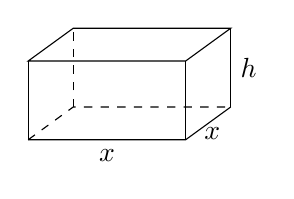
\begin{tikzpicture}  % ------ La boite sans couvercle ------------------
      [x={(-0.572cm,-0.416cm)},y={(1cm,0cm)},z={(0cm,1cm)}]
    \draw [dashed] (1,0,0)--(0,0,0) --(0,2,0) ;
    \draw  (0,2,0) --  node [pos=.8, right ] {$x$} (1,2,0)-- node [midway, below ] {$x$}(1,0,0);
    \draw (0,0,1)--(1,0,1)-- (1,2,1)-- (0,2,1)-- cycle;
    \draw [dashed] (0,0,0)--(0,0,1) ;
    \draw (1,0,0)--(1,0,1);
    \draw (0,2,0)-- node [midway, right ] {$h$}(0,2,1);
    \draw (1,2,0)-- (1,2,1);
\end{tikzpicture} & \raisebox{3ex}{ \parbox{5cm}{ Volume : $\dfrac{1}{2}$ L \\
                                  $x$ et $h$ en $cm$ \\ 
                                }} \\
\end{tabular}}

Déterminer $x$ pour que l'aire extérieure de la boîte soit minimale (parce que on veut peindre la boîte à moindre frais). \\


\begin{tabular}{l@{$\;$}l}
{\renewcommand{\arraystretch }{1.75}
\begin{tabular}{r@{$\;$}ll}
On a $\qquad \qquad \mathcal{V}$ & $ = x^2h $ & \multirow{2}{3cm}{$\left.\begin{array}{c}
                                                 \\
                                                 \\
                                                 \end{array}\right \rbrace x^2h =500$ }\\
     $\mathcal{V}$ & $ = 500 cm^3  $ &\\
                   &            &     \\
     $\scrA$ & $ = x^2 + 4xh $ & \\  
                   & $ = x^2 + 4x \dfrac{500}{x^2} $ \\
                   & $ = x^2 + \dfrac{2000}{x}  $ \\           
\end{tabular}} & \raisebox{-10ex}{\parbox{8cm}{
                     \renewcommand{\arraystretch }{1.5}
                     \begin{tabular}{r@{$\;$}l}
                      Soit $f:$ & $ \mathbb{R}\rightarrow \mathbb{R} $ \\
                                & $ x \rightarrow f(x) : x^2 + \dfrac{2000}{x}    
                                      \qquad \qquad \mathrm{D}_f = ] 0,+\infty[ $ \\
                     \end{tabular}   \\              
                        Asymptote verticale $x=0$ \\
                        \begin{tabular}{r@{$\;$}l}
                            RG de $f$ en abscisse & : 1 cm pour 5 \\
                                       en ordonnées & : 1 cm pour 100.\\
                       \end{tabular}
                       }} \\
\end{tabular}\\
\renewcommand{\arraystretch }{1}
\centerline{% \input{preambule-sacha-utf8.ltx}


% \begin{document}

\begin{tikzpicture}[line cap=round,line join=round,>=triangle 45,x=0.2cm,y=.01cm,scale=.8]
\draw[->] (-5,0) -- (45,0);
\foreach \x in {5,10,15,20,25,30,35,40}
\draw[shift={(\x,0)}] (0pt,2pt) -- (0pt,-2pt) node[below] {\footnotesize $\x$};
\draw[->] (0,-50) -- (0,1450);
\foreach \y in {,100,200,300,400,500,600,700,800,900,1000,1100,1200,1300,1400}
\draw[shift={(0,\y)}] (2pt,0pt) -- (-2pt,0pt) node[left] {\footnotesize $\y$};
\draw (0pt,-5pt) node[left] {\footnotesize $0$};
\clip(-8,-55) rectangle (50,1400);
\draw[smooth,samples=100,domain=1:50.0] plot(\x,{(\x)^2+2000/(\x)});

\begin{pgfonlayer}{background}   
\draw[step=1mm,ultra thin,AntiqueWhite!10] (-8,-55)  grid (45,1400);
\draw[step=5mm,very thin,AntiqueWhite!30]   (-8,-55)  grid (45,1400);
\draw[step=1cm,very thin,AntiqueWhite!50]   (-8,-55)  grid (45,1400);
\draw[step=5cm,thin,AntiqueWhite]          (-8,-55)  grid (45,1400);
\end{pgfonlayer} 

\end{tikzpicture}



% \end{document}
}

\newpage

Montrons que $f$ est décroissante sur $]0,10]$\\
Soit $x_1$ et $x_2 \in ]0,10] \qquad $ avec $\boxed {x_1 < x_2} $ \\

%\bigskip 

\begin{tikzpicture}  

\tikzstyle{block} = [color=darkgreen] 
%      \draw [help lines] (0,0) grid (8,5)  ; 
   \matrix 
    {
    a & b \\ 
\node {$f(x_2) - f(x_1) $} ;  & \node {$=$} ;  & \node [left=1.7cm] {$ \left({x_2}^2 + \dfrac{2000}{x_2}\right) 
                               - \left({x_1}^2 
                                 + \dfrac{2000}{x_1}\right) $ } ; \\
                 & \node {$=$} ;  &  \node [left=2.2cm] {$ {x_2}^2 + \dfrac{2000}{x_2} - {x_1}^2 
                                    - \dfrac{2000}{x_1}$ }  ; \\                              
                  & \node {$=$} ; & \node [left=.8cm]{ $ \left({x_2} - {x_1}\right) 
                            \left({x_2} + {x_1}\right) 
                            + 2000 
                               \left(\dfrac{1}{x_2} - \dfrac{1}{x_1}\right)$ }; \\    
                  & \node {$=$}; & \node [left=.2cm]{ $ \dfrac{\left({x_2} - {x_1}\right) 
                                                \left({x_2} + {x_1}\right) x_1 x_2 - 2000 
                                                \left( x_2 - x_1 \right)}      {x_1 x_2}$ } ; \\                                                  
                   &   & \node (a) {\textcolor{darkgreen}{Négatif}} ; \\                                                                                                                                          
                  & \node (b) {$=$} ;  & \node (c) [left=1.3cm]{ $ \dfrac{\left(x_2 - x_1\right) \quad \big[
                             \left({x_2} + {x_1}\right) x_1 x_2 - 2000\big]}{\quad x_1 x_2}$ } ;\\                                                                                                                                         
                  &    & \node  (d) [left=4cm] {\textcolor{darkgreen}{\parbox{2cm}{Strictement\\positif}}} ; 
                          \node (e) [left] {\textcolor{darkgreen}{\parbox{2cm}{Strictement\\positif}}} ;\\                                                                                                                        
} ; 
\draw [->, darkgreen] (a.west)  to [bend right]  (c.north); 
\draw [->, darkgreen] (d)  to [bend left]  (c.west); 
\draw [->, darkgreen] (e.north west)  to [bend left]  (c);   ; 
\end{tikzpicture} \\

\begin{itemize}
\item[*] $\left. \begin{array}{c}
                     x_1 > 0\\
                     x_2 > 0 
                 \end{array} \right\rbrace x_2 x_1 > 0 $ \\
                 
\item[*] \raisebox{-9ex}{$       \begin{array}{r@{\;}c@{\;}l}
                     x_1 & \leqslant & 10\\
                     x_2 & \leqslant & 10\\
                         &           &    \\    
              (x_2 + x_1)& \leqslant & 20\\   
                 x_1 x_2 & \leqslant & 100 \\ 
               (x_2 + x_1) x_1 x_2 & \leqslant & 2000 \\ 
(x_2 + x_1) x_1 x_2  -2000 & \leqslant & 0  \\               
                 \end{array} $  } \\

\bigskip 
                 
  Conclusion : $f(x_2) - f(x_1) \leqslant 0 $

\end{itemize}

\bigskip    

\newpage
  
Montrons que $f$ est croissante sur $]10, +\infty[$ \\
                              
Soit $x_1$ et $x_2 \in [10,+\infty \qquad $ avec $\boxed {x_1 < x_2} $ \\

\begin{tikzpicture}  
   \matrix 
    {
                   &   & \node (a) {\textcolor{darkgreen}{Positif}} ; \\                                                                                                                                          
\node {$f(x_2) - f(x_1) $} ;  & \node {$=$} ;  & \node (c) [left=1.3cm]{ $ \dfrac{\left(x_2 - x_1\right) \quad \big[
                             \left({x_2} + {x_1}\right) x_1 x_2 - 2000\big]}{\quad x_1 x_2}$ } ;\\                                                                                                                                         
                  &    & \node  (d) [left=4cm] {\textcolor{darkgreen}{\parbox{2cm}{Strictement\\positif}}} ; 
                          \node (e) [left] {\textcolor{darkgreen}{\parbox{2cm}{Strictement\\positif}}} ;\\                                                                                                                        
} ; 
\draw [->, darkgreen] (a.west)  to [bend right]  (c.north); 
\draw [->, darkgreen] (d)  to [bend left]  (c.west); 
\draw [->, darkgreen] (e.north west)  to [bend left]  (c);   ; 
\end{tikzpicture} \\


\begin{itemize}
\item[*] $\left. \begin{array}{c}
                     x_1 > 0\\
                     x_2 > 0 
                 \end{array} \right\rbrace x_2 x_1 > 0 $ \\
                 
\item[*] \raisebox{-9ex}{$       \begin{array}{r@{\;}c@{\;}l}
                     x_1 & \geqslant& 10\\
                     x_2 & \geqslant & 10\\
                         &           &    \\    
              (x_2 + x_1)& \geqslant & 20\\   
                 x_1 x_2 & \geqslant & 100 \\ 
               (x_2 + x_1) x_1 x_2 & \geqslant & 2000 \\ 
(x_2 + x_1) x_1 x_2  -2000 & \geqslant & 0  \\               
                 \end{array} $  } \\
            
\bigskip                  
  Conclusion : $f(x_2) - f(x_1) \geqslant 0 $
\end{itemize}

\bigskip    

Le minimum a donc pour coordonnées $(10, 300)$. 

L'aire maximale est donc obtenue pour $x = 10 cm$. Elle est alors de $300 cm^2$. 
